\noindent\enquote{\itshape Light thinks it travels faster than anything but it is wrong. No matter how fast light travels, it finds the darkness has always got there first, and is waiting for it. }\bigbreak

\hfill Terry Pratchet - Reaper Man

\vspace*{0.05\textheight}

In this chapter we compare the absorption spectra of Au based nanoalloys, primarily focusing on alloying with Pt as discussed in Chapter \ref{c:Introduction}. Initially, we shall make a comparrison of the three levels of theory for computing optical properties of small Au based nanoalloys: fully atomistic \textit{ab initio} methods presented in Section \ref{sec:TDDFT_Thr}; the jellium model as presented in Section \ref{sec:JML_Thr}; and the Greens Dyadic Method presented in Section \ref{sec:GDM}. We shall then present the author's contribution to the work considering the breathing of metallic nanocages as presented in \cite{Wei}. Finally we shall present the work published in \cite{JonesAuPt} which conerns the effects of Pt doping on small Au nanoparticles. 

\section{Comparing numerical tools for Au nanoparticles}
\label{Jellium}
We first present a brief study on comparing fully atomistic calculations, Jellium and GDM for different Au nanoparticles. Our comparison stands also for the dimer formation, in order to compare GDM and other available literature data. We also explore the effect of small structural changes which do not change the morphology as the radial breathing of Au-cages. Both TDDFT/Casida and GDM confirm a strong effect due to a radial motion. We then present our results for the Pt-doping of Au nanoparticles. We should note that the Jellium model does not simply offer transferable utility to the consideration of nanoalloys, hence we will shall only use the model as a means of drawing comparisons between theory levels for computing the optical spectra of Au and shall not be explicitly used for studies regarding nanoalloys.

We compare the described three numerical methods to describe the optical properties of Au NPs. For Jellium spheres, one can argue that the single 6$S^{1}$ electron of Au will be the primary contributor to the optical response and properties of the cluster. Indeed, in other works, it has not been uncommon to adopt such an approach for simple metal clusters, principally Na. To more accurately model Au, we have elected to use a Wigner-Seitz cell radius of 1.59 \AA, which has been corroborated in other studies \cite{Au_Jlm}, and initiated by John Perdew \cite{Jlm_R}. To have a more accurate representation, we have opted only to create Jellium clusters which contain a number of electrons required to fill a complete shell. However, an issue arises in that the atomic shell closure, and electronic shell closure, do not always coincide, and so there is often a discrepancy on the order of a few to tens of electrons between the atomistic clusters, and the Jellium. 

Nonetheless, this study is intended to probe a size range largely unobtainable by DFT methods due to the number of electrons involved. We begin by evaluating the variation in photo-absorption spectrum with respect to size and morphology with the coarsest tool at our disposal - the GDM method which is informed exclusively by atomic coordinates and corresponding specie as discussed in Section \ref{sec:GDM}.

\subsection{Atomistic model - Variation in morphology}
\label{sec:Res_Atom}
As was discussed in Sec. \ref{sec:Theory_DFT}, the accurate implementation of DFT and TDDFT methods can often appear to be more of an art than an exact science. As such, we have elected to begin our investigations with \texttt{Octopus} \cite{Octopus2003,Octopus_2006,Oct_paralel,Oct_2015,Oct_2020} with caution and the general objective of determining what is feasible, physical, and numerically cost-effective. To be precise, we shall primarily be concerned with properties such as the density of states (DoS) which yields electrotatic information; the optical extinction spectrum which may be compared against experimental data and computations arising from other levels of theory.

We begin by computing the optical extinction spectrum for a small Au$_{14}^{Cb}$ cluster. Comparing the simple LDA pseudopotential set \cite{PhysRevB.58.3641}, a modern set of Optimised Norm-Conserving Vanderbilt PBE pseudopotentials \cite{SCHLIPF201536}, and a set provided by the Fritz Haber Institute where the former two sets may be considered to be 'out of the box' as they come pre-compiled with LibXC \cite{LibXC} when building \texttt{Octopus}. We do not compare the density of states for these sets as it is self evident given the number of core and valence electrons considered in each set that only approximate features will appear consistent for such a small cluster. However, given that the objective in the broader research project is to evaluate the optical performance, then extinction spectra are a more meaningful set of quantities to consider for comparison.

\begin{table}[ht]
\centering
\caption{Au valence electrons for each psuedpotential set.}
\label{tab:pseudos}
\begin{tabular}{@{}lll@{}}
\toprule
Type & Functional & Valence electrons  \\
\hline
HGH & LDA \cite{PhysRevB.58.3641} &  6$s^{1}$   \\ \\
FHI & LDA \cite{FHI}  &  5d$^{10}$6s$^{1}$   \\ \\
Norm-Conserving Vanderbilt & GGA \cite{SCHLIPF201536} &   5$s^{2}$5p$^{6}$5$d^{10}$6$s^{1}$    \\ \\
\bottomrule
\end{tabular}
\end{table}

\begin{figure}
    \centering
    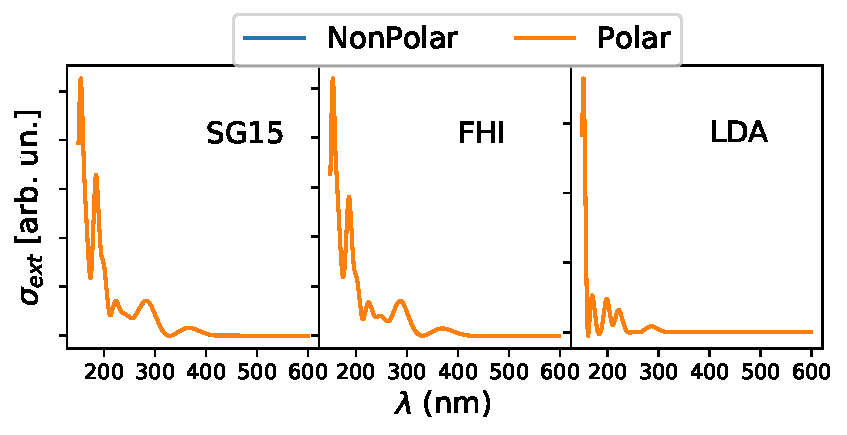
\includegraphics[width=0.8\textwidth]{figures/LM/Atomistic/PPs_Compare.pdf}
    \caption{Comparison of the pseudopotentials presented in Table \ref{tab:pseudos} with both the spin polarised and unpolarised cases presented for the Au$_{14}^{Cb}$ structure as a test case. All spectra computed via the TDDFT method by calculating Equation \ref{eqn:DFTSigma} as described in Section \ref{sec:RTTDDFT}.}
    \label{fig:pps}
\end{figure}

Given the apparent similarity between the pseudopotentials examined in Figure \ref{fig:pps}, and Table \ref{tab:pseudos}, and the relative lack of influence that performing spin polarised calculations had over those which were unpolarised, we elected to proceed with the cheapest possible set of input parameters so as to increase the efficiency of the calculation - albeit at some cost to accuracy given the increased number of approximations. We note that there are indeed some deviations between the HGH and the more expensive pseudopotentials, which we shall take into consideration in the more comprehensive study later in this chapter. Nonetheless, the main feature of the sharp peak at $\sim$ 150 nm is present in all of the spectra computed. It is likely that the additional lower energy peaks in the spectra are due to richer electron density oscillations contributing to the absorption spectrum computed via Equation \ref{eqn:DFTSigma}. Therefore, we shall continue to use the cheaper pseudopotentials when considering the influence that morphology has on the electron density of states (DoS) and extinction spectra. 

In proceeding, we generated a small subset of sub nanometer Au NPs whose number of atomic constituents ranged from 13 to 19. We must acknowledge here that it is generally accepted that the transition from planar to three dimensional with respect to the number of atoms for Au is between 12 to 14. This argument has been substantiated from an energetic perspective and corroborated with DFT calculations \cite{doi:10.1063/1.1507582,doi:10.1021/jp035437i}. Consequently, we must acknowledge that the structures presented do not necessarily satisfy the condition of occupying a minimum in the potential energy landscape. Nonetheless, a beautiful element within nanoscience is the vast fluxionality that may be observed, and that a cluster will not necessarily be in the configurational ground state at any given time. This is further supported by the argument that the conditions in which such clusters may be created and measured, for example via time of flight spectroscopy \cite{PierroDoping}, are not necessarily those which favour existing in the ground state. Moreover, the purpose of these calculations is not to be idealistic, rather to determine how small fluxional variations may influence spectral response functions. Information which is important to have during experimental procedures as the aggregate of a given spectrum will be constructed from all of the nanoparticles in the sample with each contributing in its own beautifully diverse fashion.

\begin{figure}
\centering
    \begin{subfigure}{0.29\textwidth}
        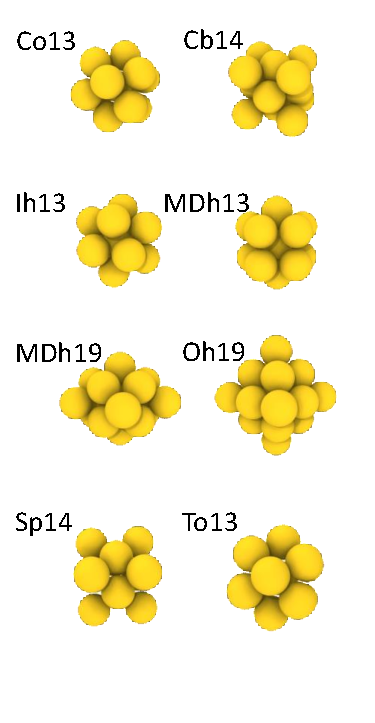
\includegraphics[width=\textwidth]{figures/LM/Atomistic/Struts.pdf}
        \caption{Structures considered.}
        \label{fig:AuNPs_Struts}
    \end{subfigure}
    \begin{subfigure}{0.335\textwidth}
        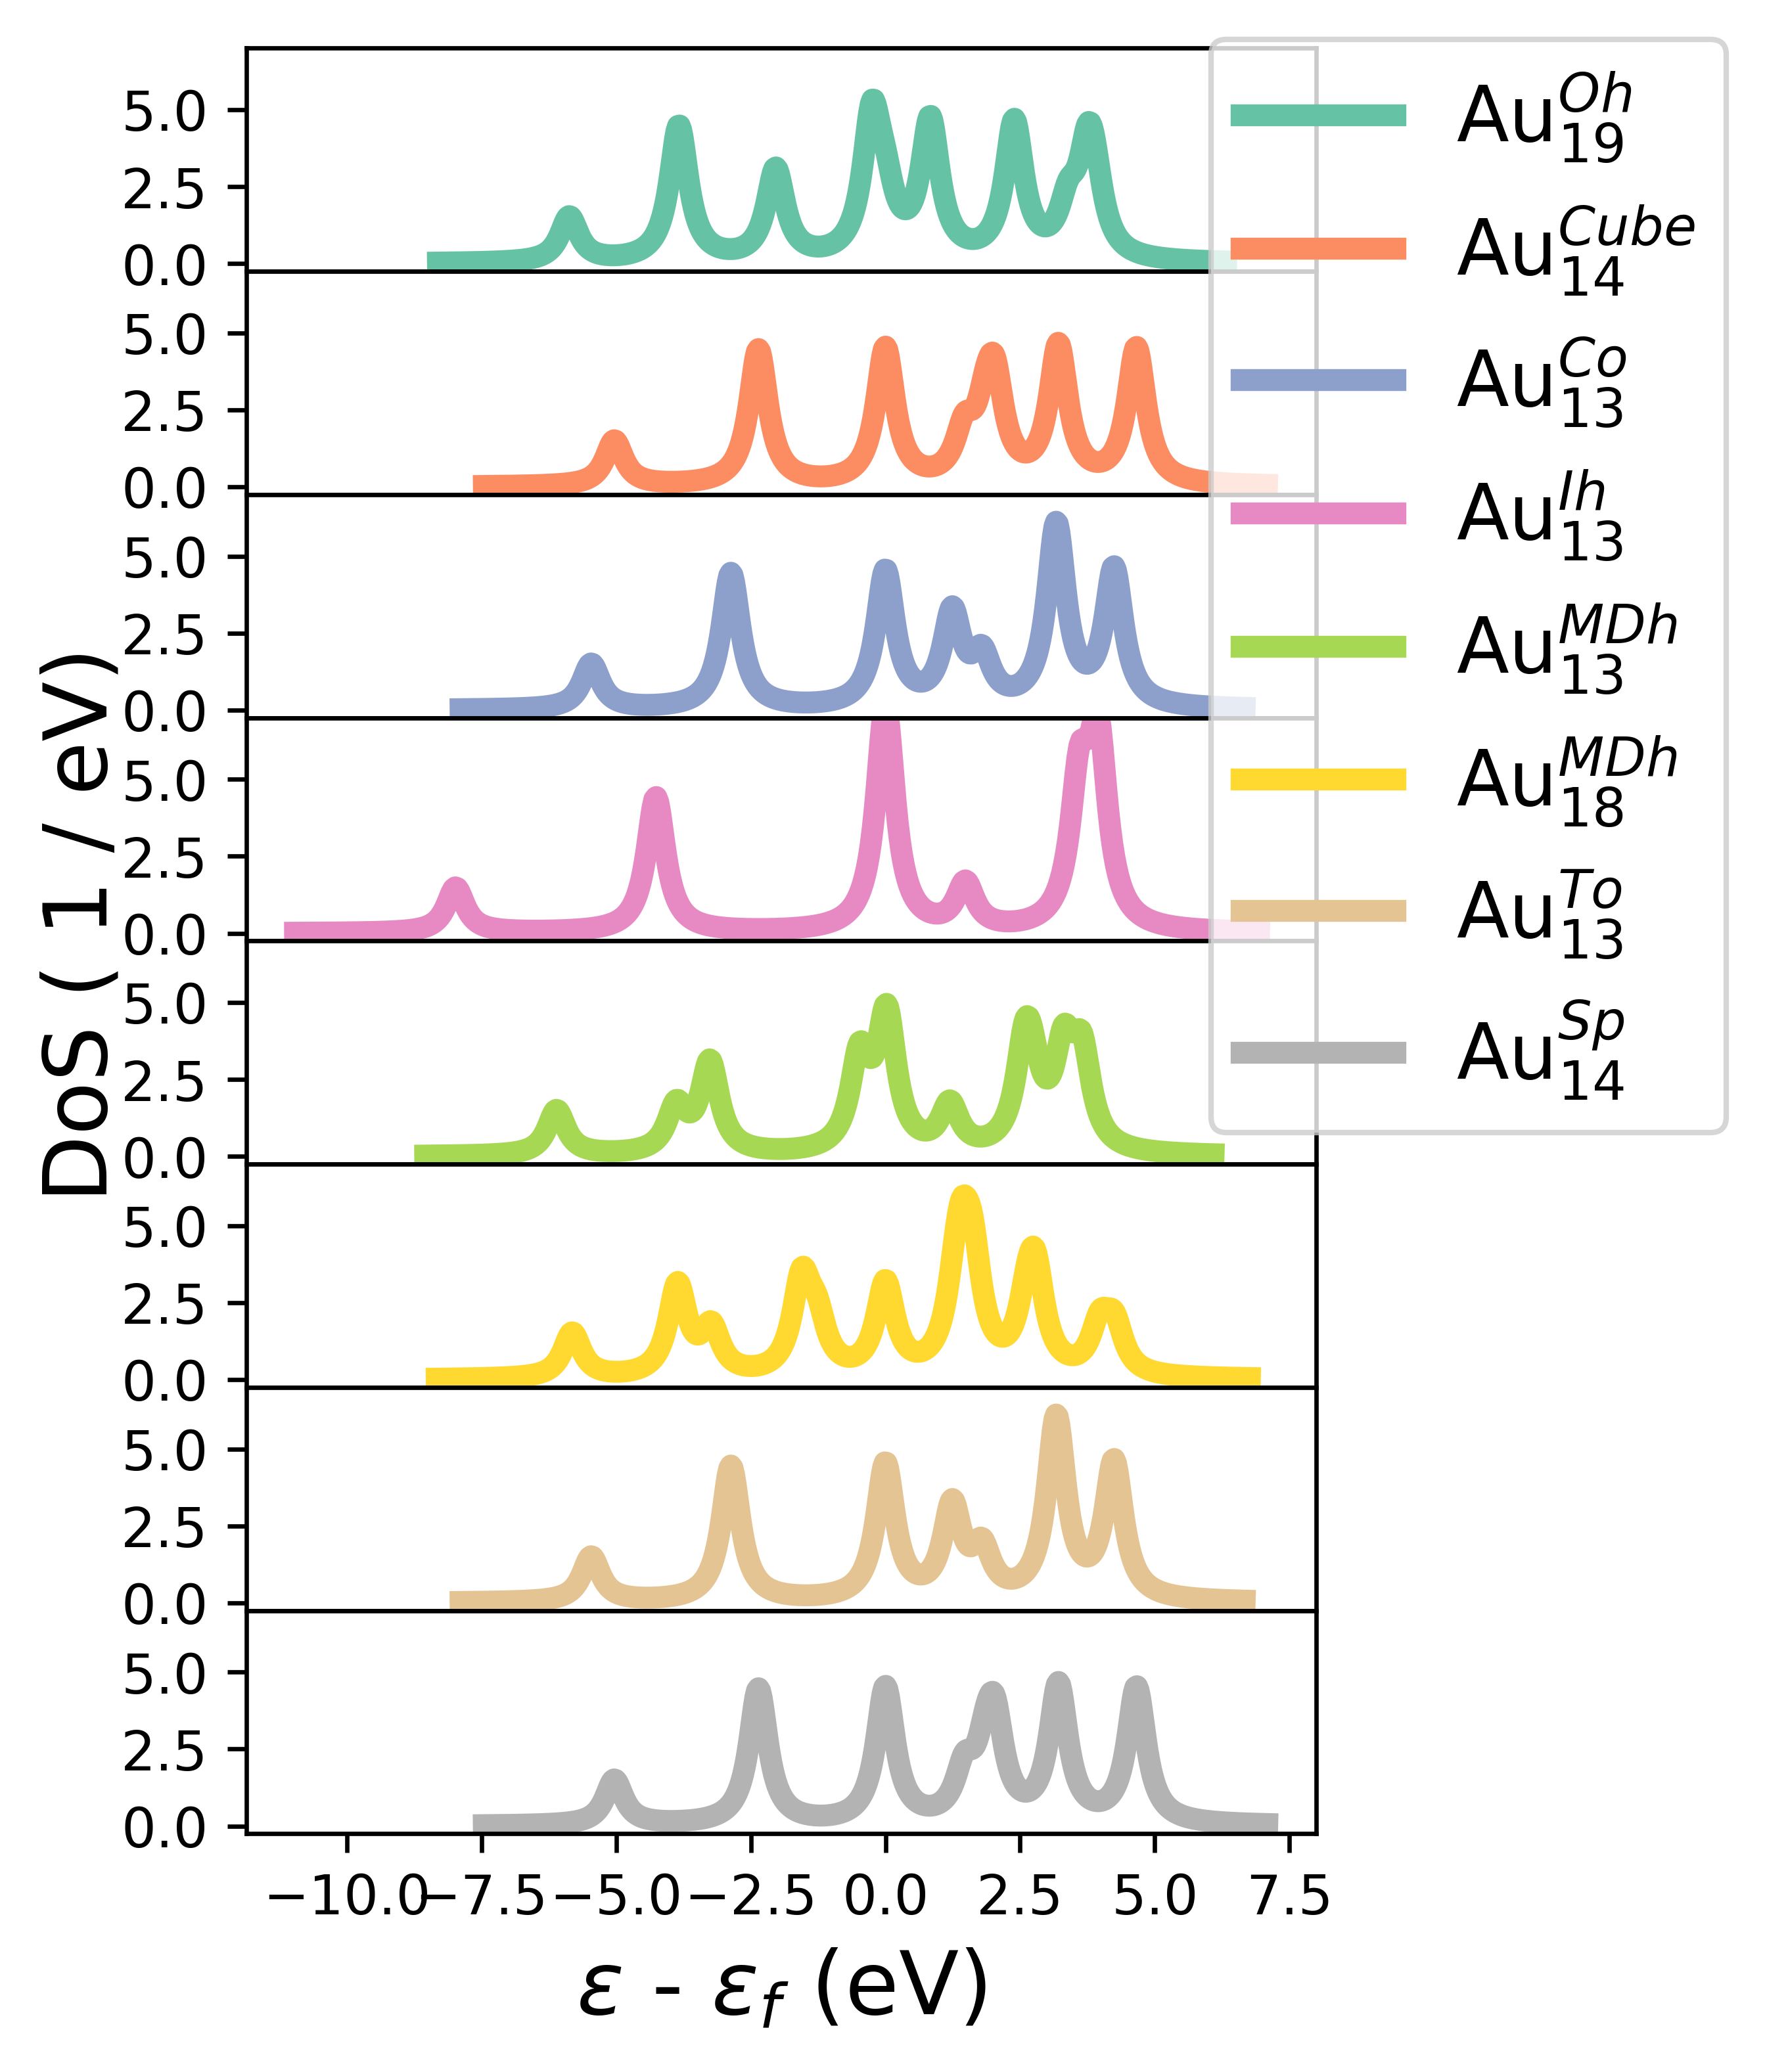
\includegraphics[width=\textwidth]{figures/LM/Atomistic/Au_NPs_DoS.png}
        \caption{DoS.}
        \label{fig:AuNPs_DoS}
    \end{subfigure}
    \begin{subfigure}{0.335\textwidth}
        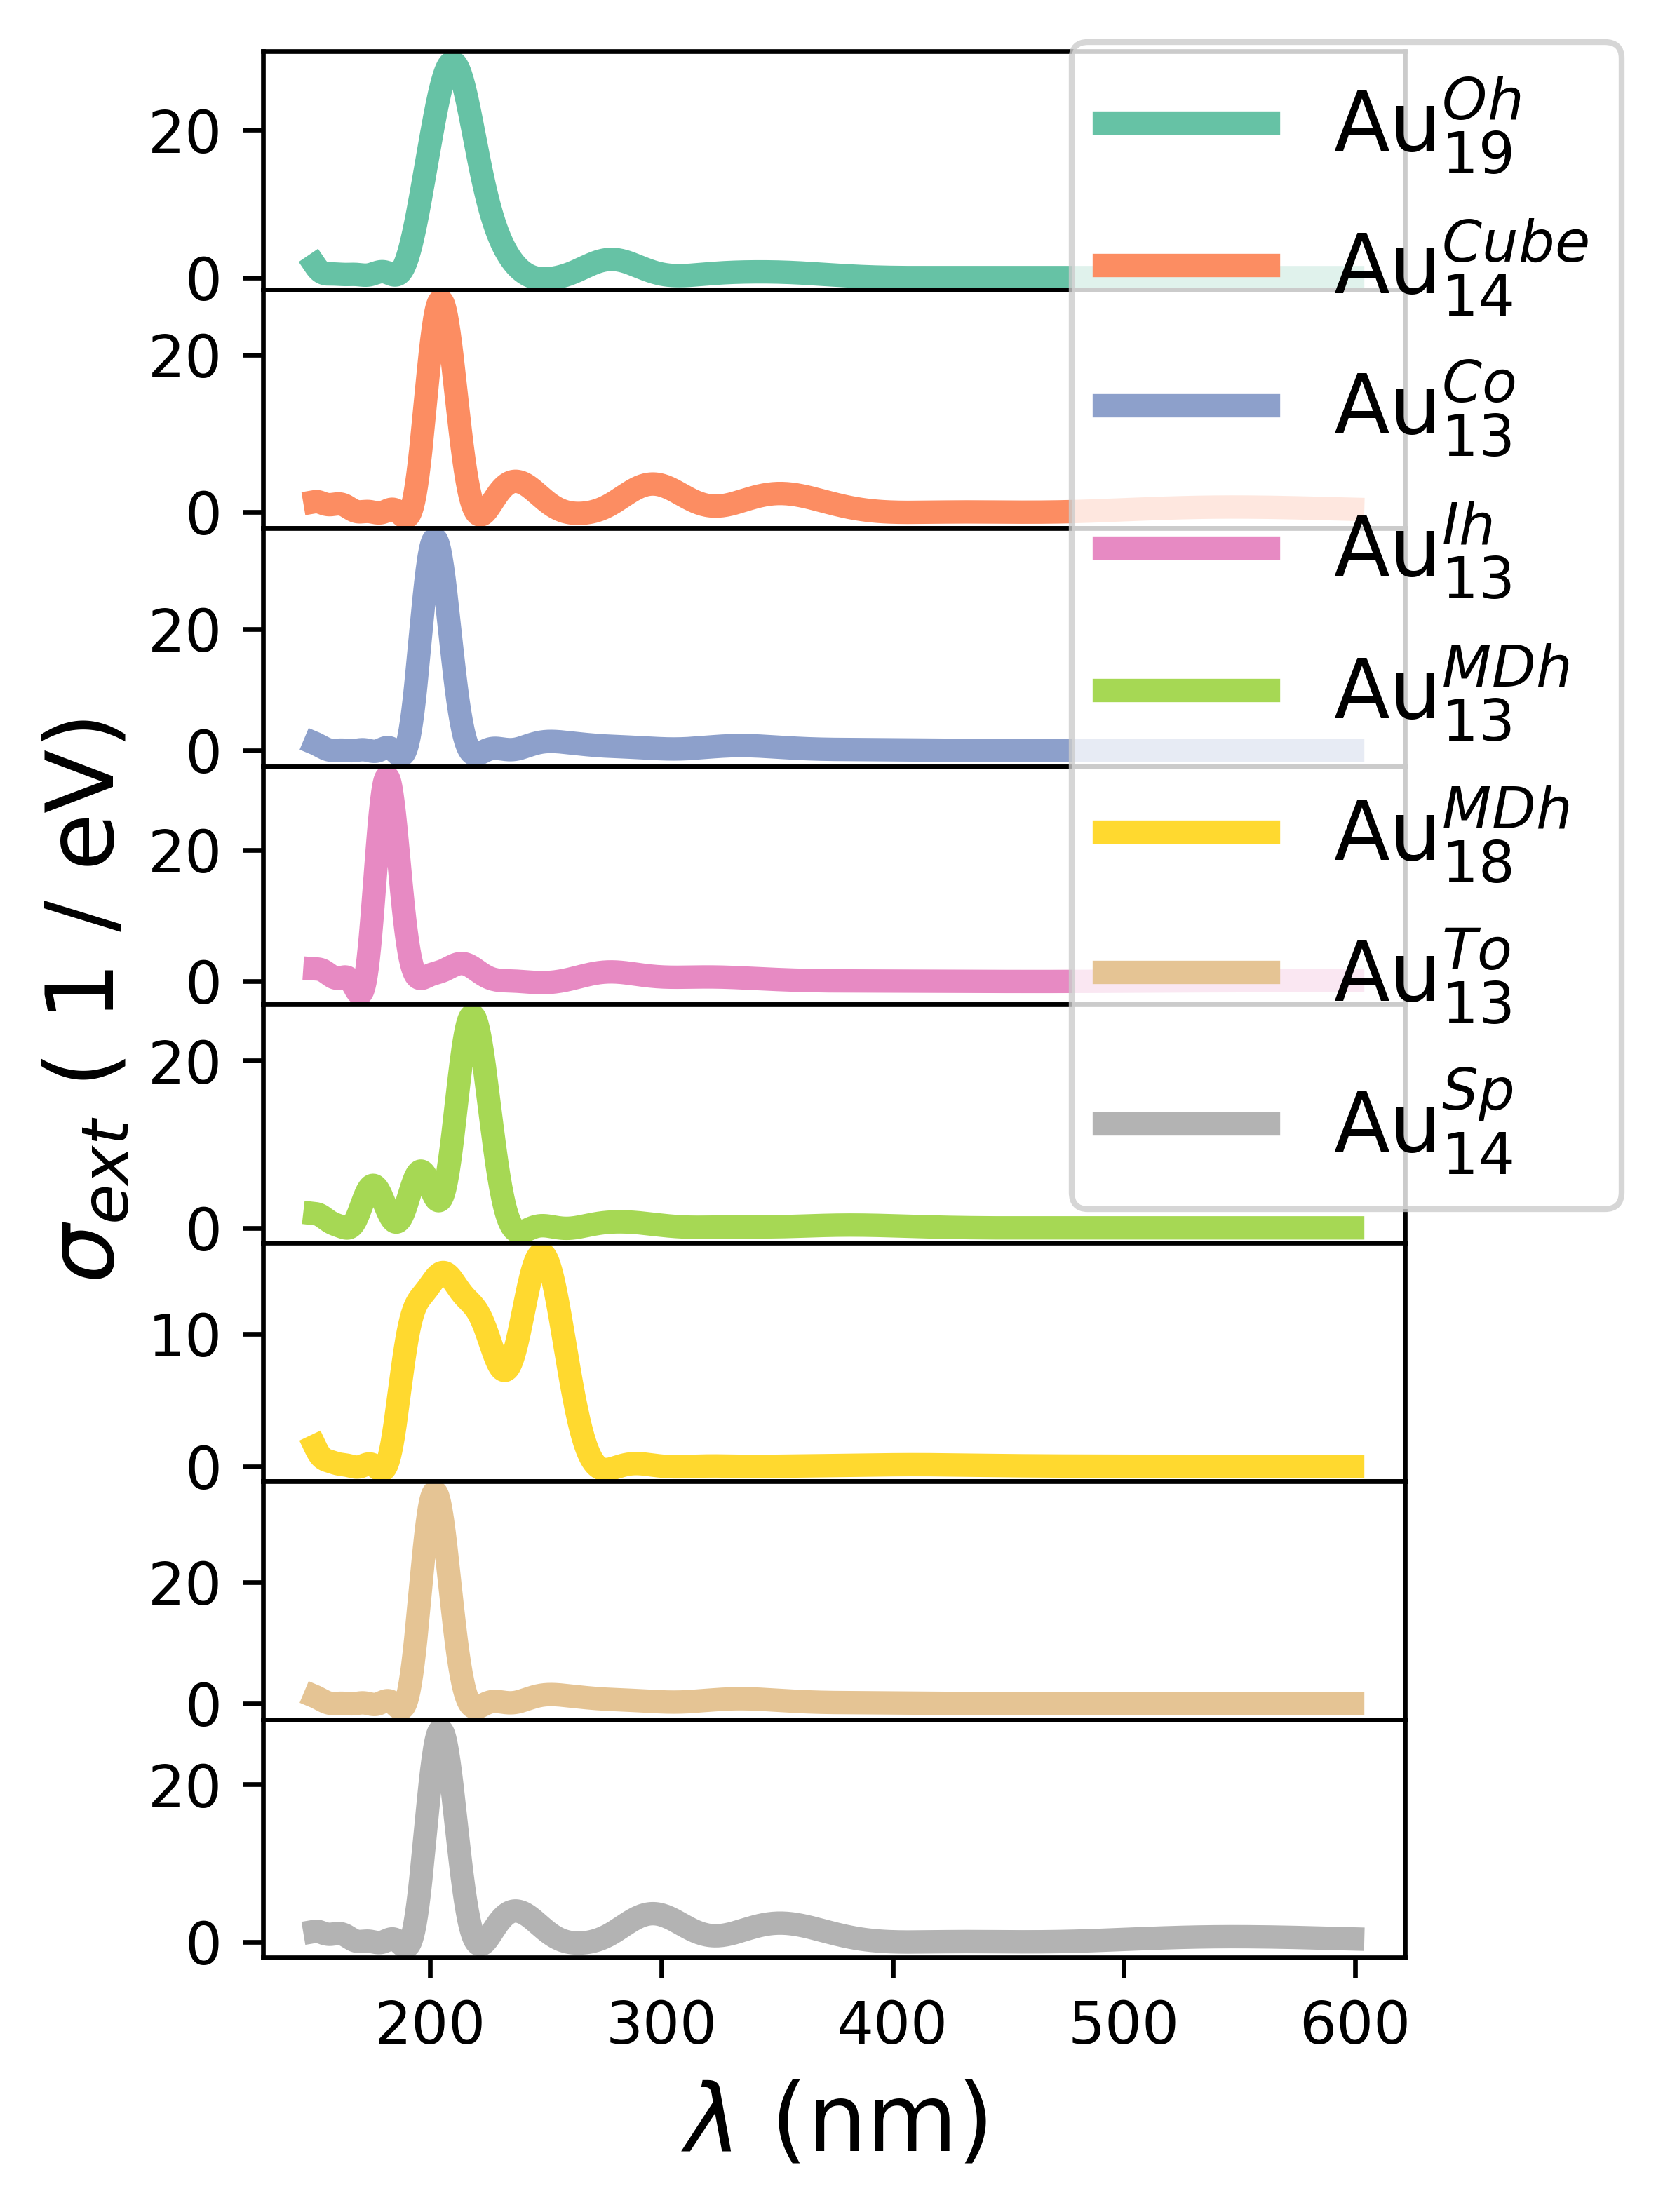
\includegraphics[width=\textwidth]{figures/LM/Atomistic/Au_NPs_CSV.png}
        \caption{Extinction spectra.}
        \label{fig:AuNPs_CSV}
    \end{subfigure}
    \caption{Opto-electronic properties for small Au NPs to evaluate how small variations in morphology and size may influence calculable quantities.}
    \label{fig:DFT_AuNPs}
\end{figure}

\begin{table}[ht]
\centering
\caption{Symmetry point groups associated with clusters presented in Figure \ref{fig:AuNPs_Struts}.}
\label{tab:symmetry_groups}
\begin{tabular}{@{}llll@{}}
\toprule
Cluster Type & Schoenflies &  Order \\
Co           & I$_{h}$              & 120 \\
Cb           & O$_{h}$              & 48  \\
Ih           & I$_{h}$              & 120 \\
MDh          & D$_{5h}$             & 20  \\
Oh           & O$_{h}$              & 48  \\
Sp           & O$_{h}$              & 48  \\
To           & I$_{h}$              & 120 \\
Th           & T$_{d}$              & 24  \\
\hline
\bottomrule
\end{tabular}
\end{table}

We demonstrate in Figure \ref{fig:DFT_AuNPs} the impact of fluxionality discussed above. Here, the geometric configuration itself will visibly alter how the available electronic states are arranged and distributed within the nanoparticle. Indeed, one is able to see that structures with higher symmetries: Ih, Co, and Sp appear to have a more strongly discretised density of states when compared to those of more exotically shaped structures such as the MDh, Oh, and To. One could posit that the high levels of spatial symmetry allow for a more ordered electronic configuration in the available state space, with orbitals being stabilised at regular and consistent intervals within the spatial landscape which likely then corresponds to regular and consistent spacing within the state-space landscape. Furthermore, one cannot neglect the behaviour at and around the HOMO, the x-axis zero of Figure \ref{fig:AuNPs_DoS}, in that there appear to be two categories of clusters: those whose DoS is continuous and non-zero at the HOMO; and those whose DoS features a non~-~zero HOMO~-~LUMO gap.

As alluded to, a natural language in which to interpret the DoS and absorption spectra displayed in Figure \ref{fig:DFT_AuNPs} is that of symmetry operations, and the richness of the symmetry associated with the specific cluster. This is not a novel approach, as arguments relating symmetry with electronic structure are ubiquitous and abundant with the nanoparticle modelling community \cite{doi:10.1021/acs.jpca.8b07923,PhysRevB.84.035325,doi:10.1021/acs.jpcc.9b05863,C9NR08515G,PhysRevB.81.233407}. In Table \ref{tab:symmetry_groups} we have presented the pure Au clusters which are considered in this chapter, their associated symmetry group as denoted by their Schoenflies notation, and the order of that symmetry group \cite{jacobs_2005}. 

We motivate the inclusion of the Cb and Sp into O$_{h}$ group as the cube has octahedral symmetry as a platonic solid, and the chosen geometry for the spherical MNP was carved from a larger Oh MNP. As for the MNPs whose symmetry group is identified with the I$_{h}$ symmetry; despite both the Co and To being Archimedean solids with full O$_{h}$ symmetry, their geometries at the given size are more consistent with the I$_{h}$ symmetry group given the lack of well~-~defined facets. This is clear to see on visual inspection of the MNPs in Figure \ref{fig:AuNPs_Struts}. Finally, the MDh structures exhibit a much poorer decahedral symmetry.

Having performed classification by symmetry, we may now proceed to inspect the impact of being described by a specific symmetry group, and the order of that group. Our first observation is that clusters who may be represented by the I${_h}$ group, whose order is 120, appear to have the sharpest and most defined peaks in both their DoS and absorption spectra. Subsequently, those clusters described by the weaker O$_{h}$ group of order 48 have more features appearing in their respective DoS and spectra. These features are defined by additional subsequent peaks in their absorption spectra, and a rougher DoS landscape. Finally, the poorer D$_{5h}$ clusters have the greatest number of additional features in both their DoS and spectra. Where the larger MDh cluster features a partial splitting in its absorption spectra at $\sim$ 250 nm, and a much broader DoS relative to clusters whose corresponding symmetry groups have much higher orders.

Considering now the computed extinction spectra in Figure \ref{fig:AuNPs_CSV}, we see a similar kind of interaction between symmetry and smoothness of the function. Generally speaking, the structures discussed earlier with more profound spatial symmetries appear to have sharper single peaks with smaller residual oscillations deep into the visible range from $\sim$ 250 nm and up. With that, we must acknowledge the extreme high energy of the primary extinction peaks at 200 nm. Considering that the bulk plasmon resonance for Au is at approximately 540 nm \cite{AuPlasmonRev} and contrasting with these reported extinction spectra. However, this is not necessarily as alarming as it may otherwise appear, in that it is highly unlikely at this size and indeed with the number of elctrons present, that we expect to see true plasmon like behaviour. It is speculated that approximately 250 atoms ($\sim$ 2 nm) are necessary for the collective motion of the excited valence electrons to be plasmon like \cite{SmallPlasmonBad}. Until this transition point, the single state excitations may indeed behave collectively, but they are still fundamentally discrete in their quantity. An alternative lens that one may cast on these data is to consider the phenomena discussed in Sec. \ref{sec:plasmons} whereby the retarding force acting on the oscillating valence electrons scales with the curvature of the nanoparticle - or alternatively - is inversely proportional to the size. Therefore, as the structure shrinks, simple electromagnetic arguments require there to be an increase in the energy necessary to achieve resonance with respect to the electron distribution oscillating.


 Having established the utility of \texttt{Octopus} to make predictions regarding simple spectroscopic properties such as the DoS and the extinction spectrum, we now wish to test its utility in handling alloyed structures. As has been common insofar, we are primarily concerned with the introduction of Pt to Au. As before, we use the simplified, cheap LDA pseudopotentials for this investigation into the influence that alloying may have on opto-electronic properties. We initially consider the Core-Shell morphology, a well studied chemical ordering for AuPt nanoalloys \cite{nano9111644,5257275,https://doi.org/10.1002/ppsc.201700401,doi:10.1021/acsami.9b10158,Namsoon2021}. We shall expand more fully on the unique structural properties of Core-Shell AuPt in Chapter \ref{c:Alloy} and in Chapter \ref{c:Water}, however, for now we shall simply observe that it is the most structurally similar cluster to those presented in \cite{JorgeStructure,Jorge2019} that we could reasonably design and model at the DFT level of theory. As before, we compute both the electronic DoS and the extinction spectrum for the cluster. We proceed to do so for the separate components of the cluster, too: the Au$_{13}^{Ih}$ core and the Pt$_{42}$ shell as shown in Figure \ref{fig:DFT_CS}.

\begin{figure}
\centering
    \begin{subfigure}{0.45\textwidth}
        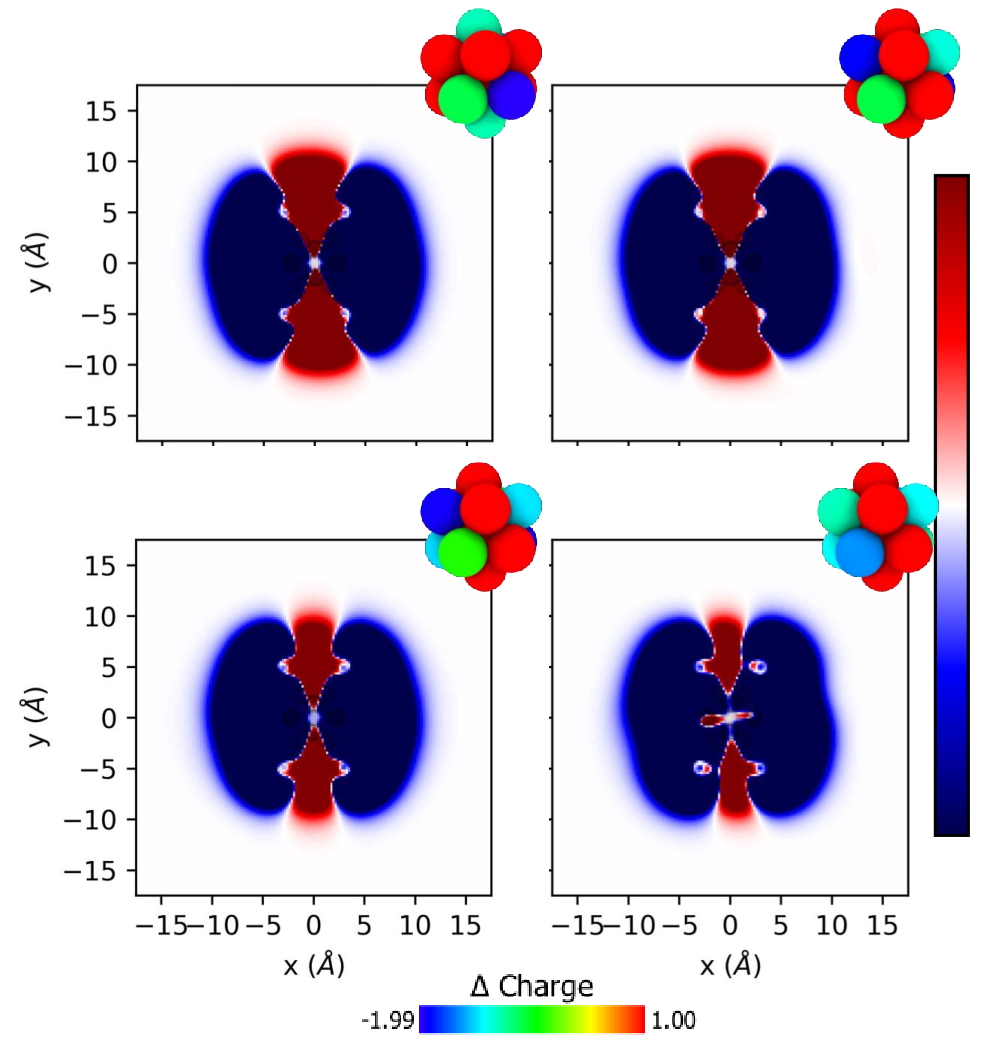
\includegraphics[width=\textwidth]{figures/LM/Atomistic/Au13_Dense.pdf}
        \caption{Au$_{13}^{Ih}$.}
        \label{fig:Au13_Dense}
    \end{subfigure}
    \begin{subfigure}{0.45\textwidth}
        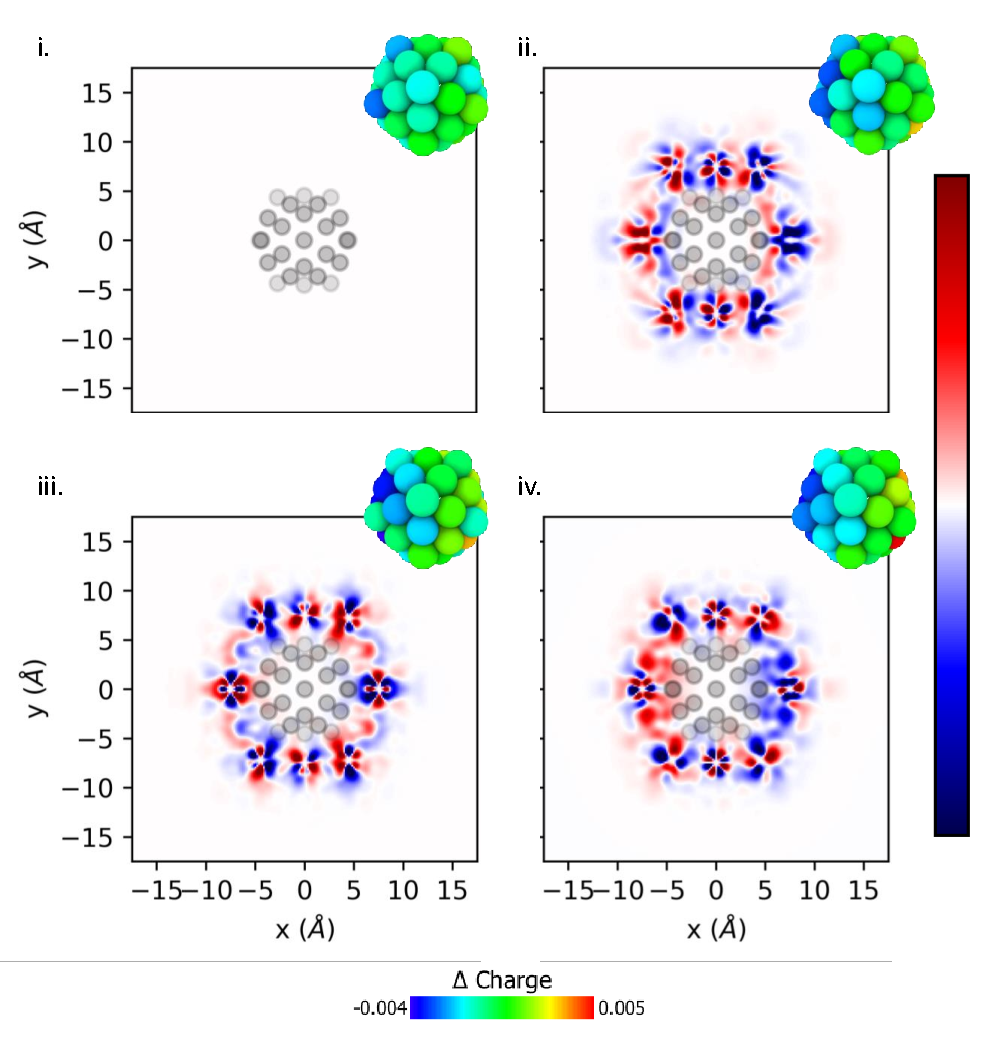
\includegraphics[width=\textwidth]{figures/LM/Atomistic/Py42_Dense.pdf}
        \caption{Pt$_{42}^{Shell}$.}
        \label{fig:CS_Dense}
    \end{subfigure}
    \begin{subfigure}{0.45\textwidth}
    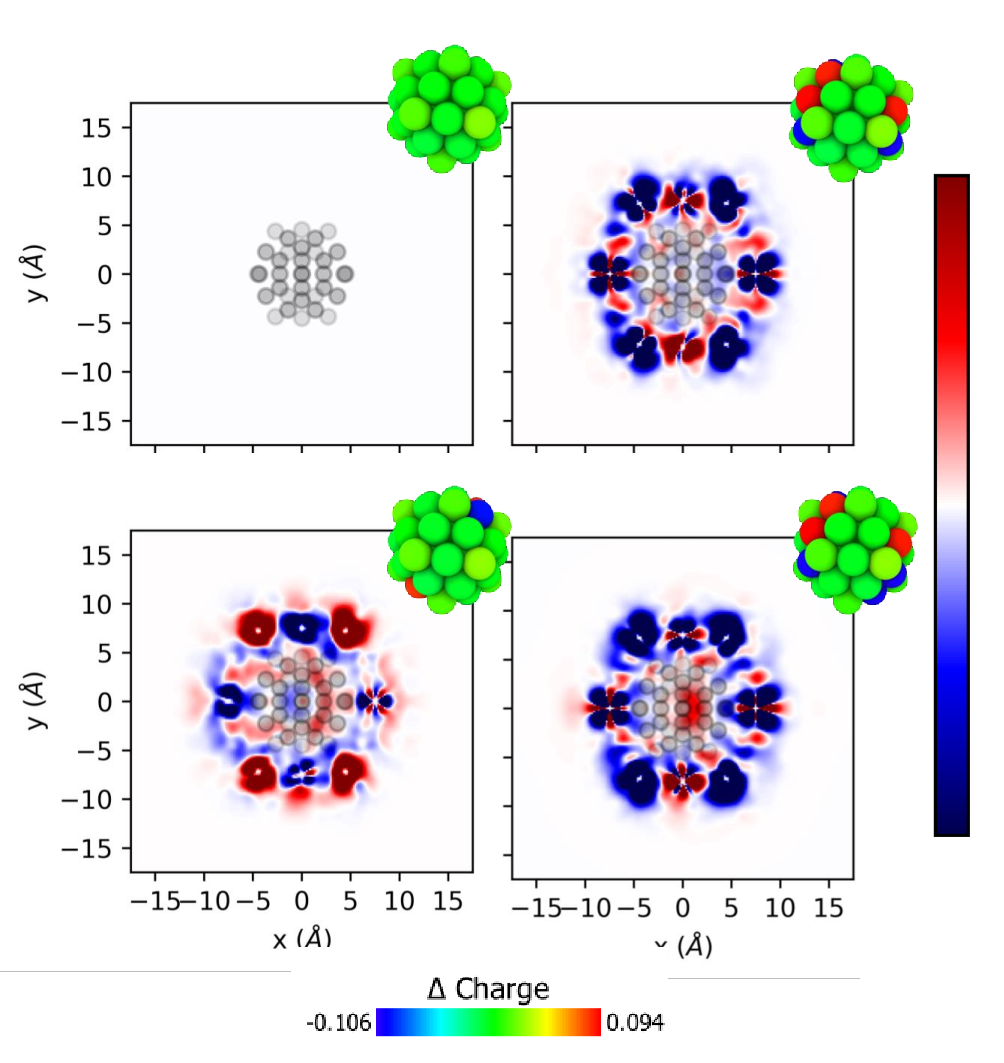
\includegraphics[width=\textwidth]{figures/LM/Atomistic/Alloy_Dense.pdf}
    \caption{Au$_{13}^{Ih}$Pt$_{42}^{Shell}$.}
    \label{fig:CS_TD}
\end{subfigure}
    \caption{Evolution of the electron density of an Au$_{13}^{Ih}$ nanoparticle following an instantaneous $delta$-kick perturbation. Vertical colour bar corresponds to the $xy$ plane heat-map and scales from $-10^{-5}$ - $10^{-5}$ which may be interpreted as having an iso-surface of the same value. Horizontal colour bar is for comparing the relative change in the Bader charges computed on each atom at the corresponding frame it is attached to. Panels \textit{i.}, \textit{ii.}, \textit{iii.}, and \text{iv.} respectively correspond to t=$0_{+}$ just following the perturbation, 0.82 femtoseconds, 3.20 femtoseconds, 6.58 femtoseconds, and 9.87 femtoseconds. \textbf{a}) Au$_{13}^{Ih}$ core. (\textbf{b}) Pt$_{42}^{Shell}$. (\textbf{c}) Au$_{13}^{Ih}$Pt$_{42}^{Shell}$. All calculations performed with the HGH class of pseudopotentials \cite{PhysRevB.58.3641} at the LDA level of theory.}
    \label{fig:DFT_CS_Dense}
\end{figure}

We present in Figure \ref{fig:DFT_CS_Dense} the evolution of the induced electronic motion of the Core-Shell cluster and its species-wise components. Included in each sub-figure are atomic representations of the change in the Bader charges \cite{doi:10.1021/ar00109a003} relative to the initial charge distribution for each cluster which have been colour coded blue to indicate an electron poor region and red for electron rich.

By Bader analysis, we refer to the identification of a zero flux surfaces, where the perpendicular charge density is minimum to divide atoms \cite{doi:10.1021/ar00109a003}. Typically in molecular systems, the charge density reaches a minimum between atoms and this is a natural place to separate atoms from each other. In this work, the charge enclosed within the Bader volume is used as an approximation to the total electronic charge of an atom. 

We may first appreciate in Figure \ref{fig:Au13_Dense} the intense response of the Au cluster to the perturbation, as indicated by the deep colouration of the charge density and further substantiated by the scale of the charge redistribution as indicated by the Bader analysis. This is indeed indicative of motion for the electron cloud in what appears to be a concerted and collective fashion - hallmark signatures of plasmon excitations. To perform Bader analyis, we have used a code prepared by Tang \textit{et al} \cite{Bader}.

Furthermore, we see that relative to Au, the Pt shell in Figure \ref{fig:CS_Dense} appears to be relatively optically inert where any oscillatory motion of the electrons appears to be purely local around each given atom. This, too, is supported by the small scale required to observe any changes with respect to the Bader charges where any changes are essentially negligable suggesting that any electron motion is indeed purely local as suggested in the density plots. This is not surprising, as Pt is not known for its vibrant optical features as Au is.

However, when we introduce an Au core to the Pt shell, we note that the scale in which electrons may begin to be seen to oscillate between atoms appears to increase by a factor of 10 as seen in the $\Delta$ Charge scale bar in Figure \ref{fig:CS_TD} and indeed as we see in the accompanying density distribution plots, there is evidence of increased charge motion which corroborates the observation made from the Bader analysis. Furthermore, it appears that the majority of the charge oscillations appear on the external region of the cluster, \textit{i.e.,} Pt instead of at the core where the Au has been placed. This would appear to suggest that the presence of an Au core incites the surface electrons of Pt to undergo a more plasmon-like oscillation. However, it is also clear that these oscillations are not concerted or collective as regions of increased and decreased electron density are still localised and fragmented - unlike the Au in Figure \ref{fig:Au13_Dense}.

Finally, it is worth noting that the electron density will continue to oscillate far longer than we have been able to compute for and present in this work. This is motivated by Figure \ref{Fig:Plasmonics}, and supported by Reference \cite{AuPlasmonRev} wherein the mechanism of Landau damping may take on the order of hundreds of fs to occur ~-~ an order of magnitude longer than has been presented here. However, convergence of the absorption spectrum, as shown in Figure \ref{fig:DFT_CS}, suggests that we have successfully identified the dominant dipole modes contributing to the absorption presented.

\begin{figure}
\centering
    \begin{subfigure}{0.45\textwidth}
        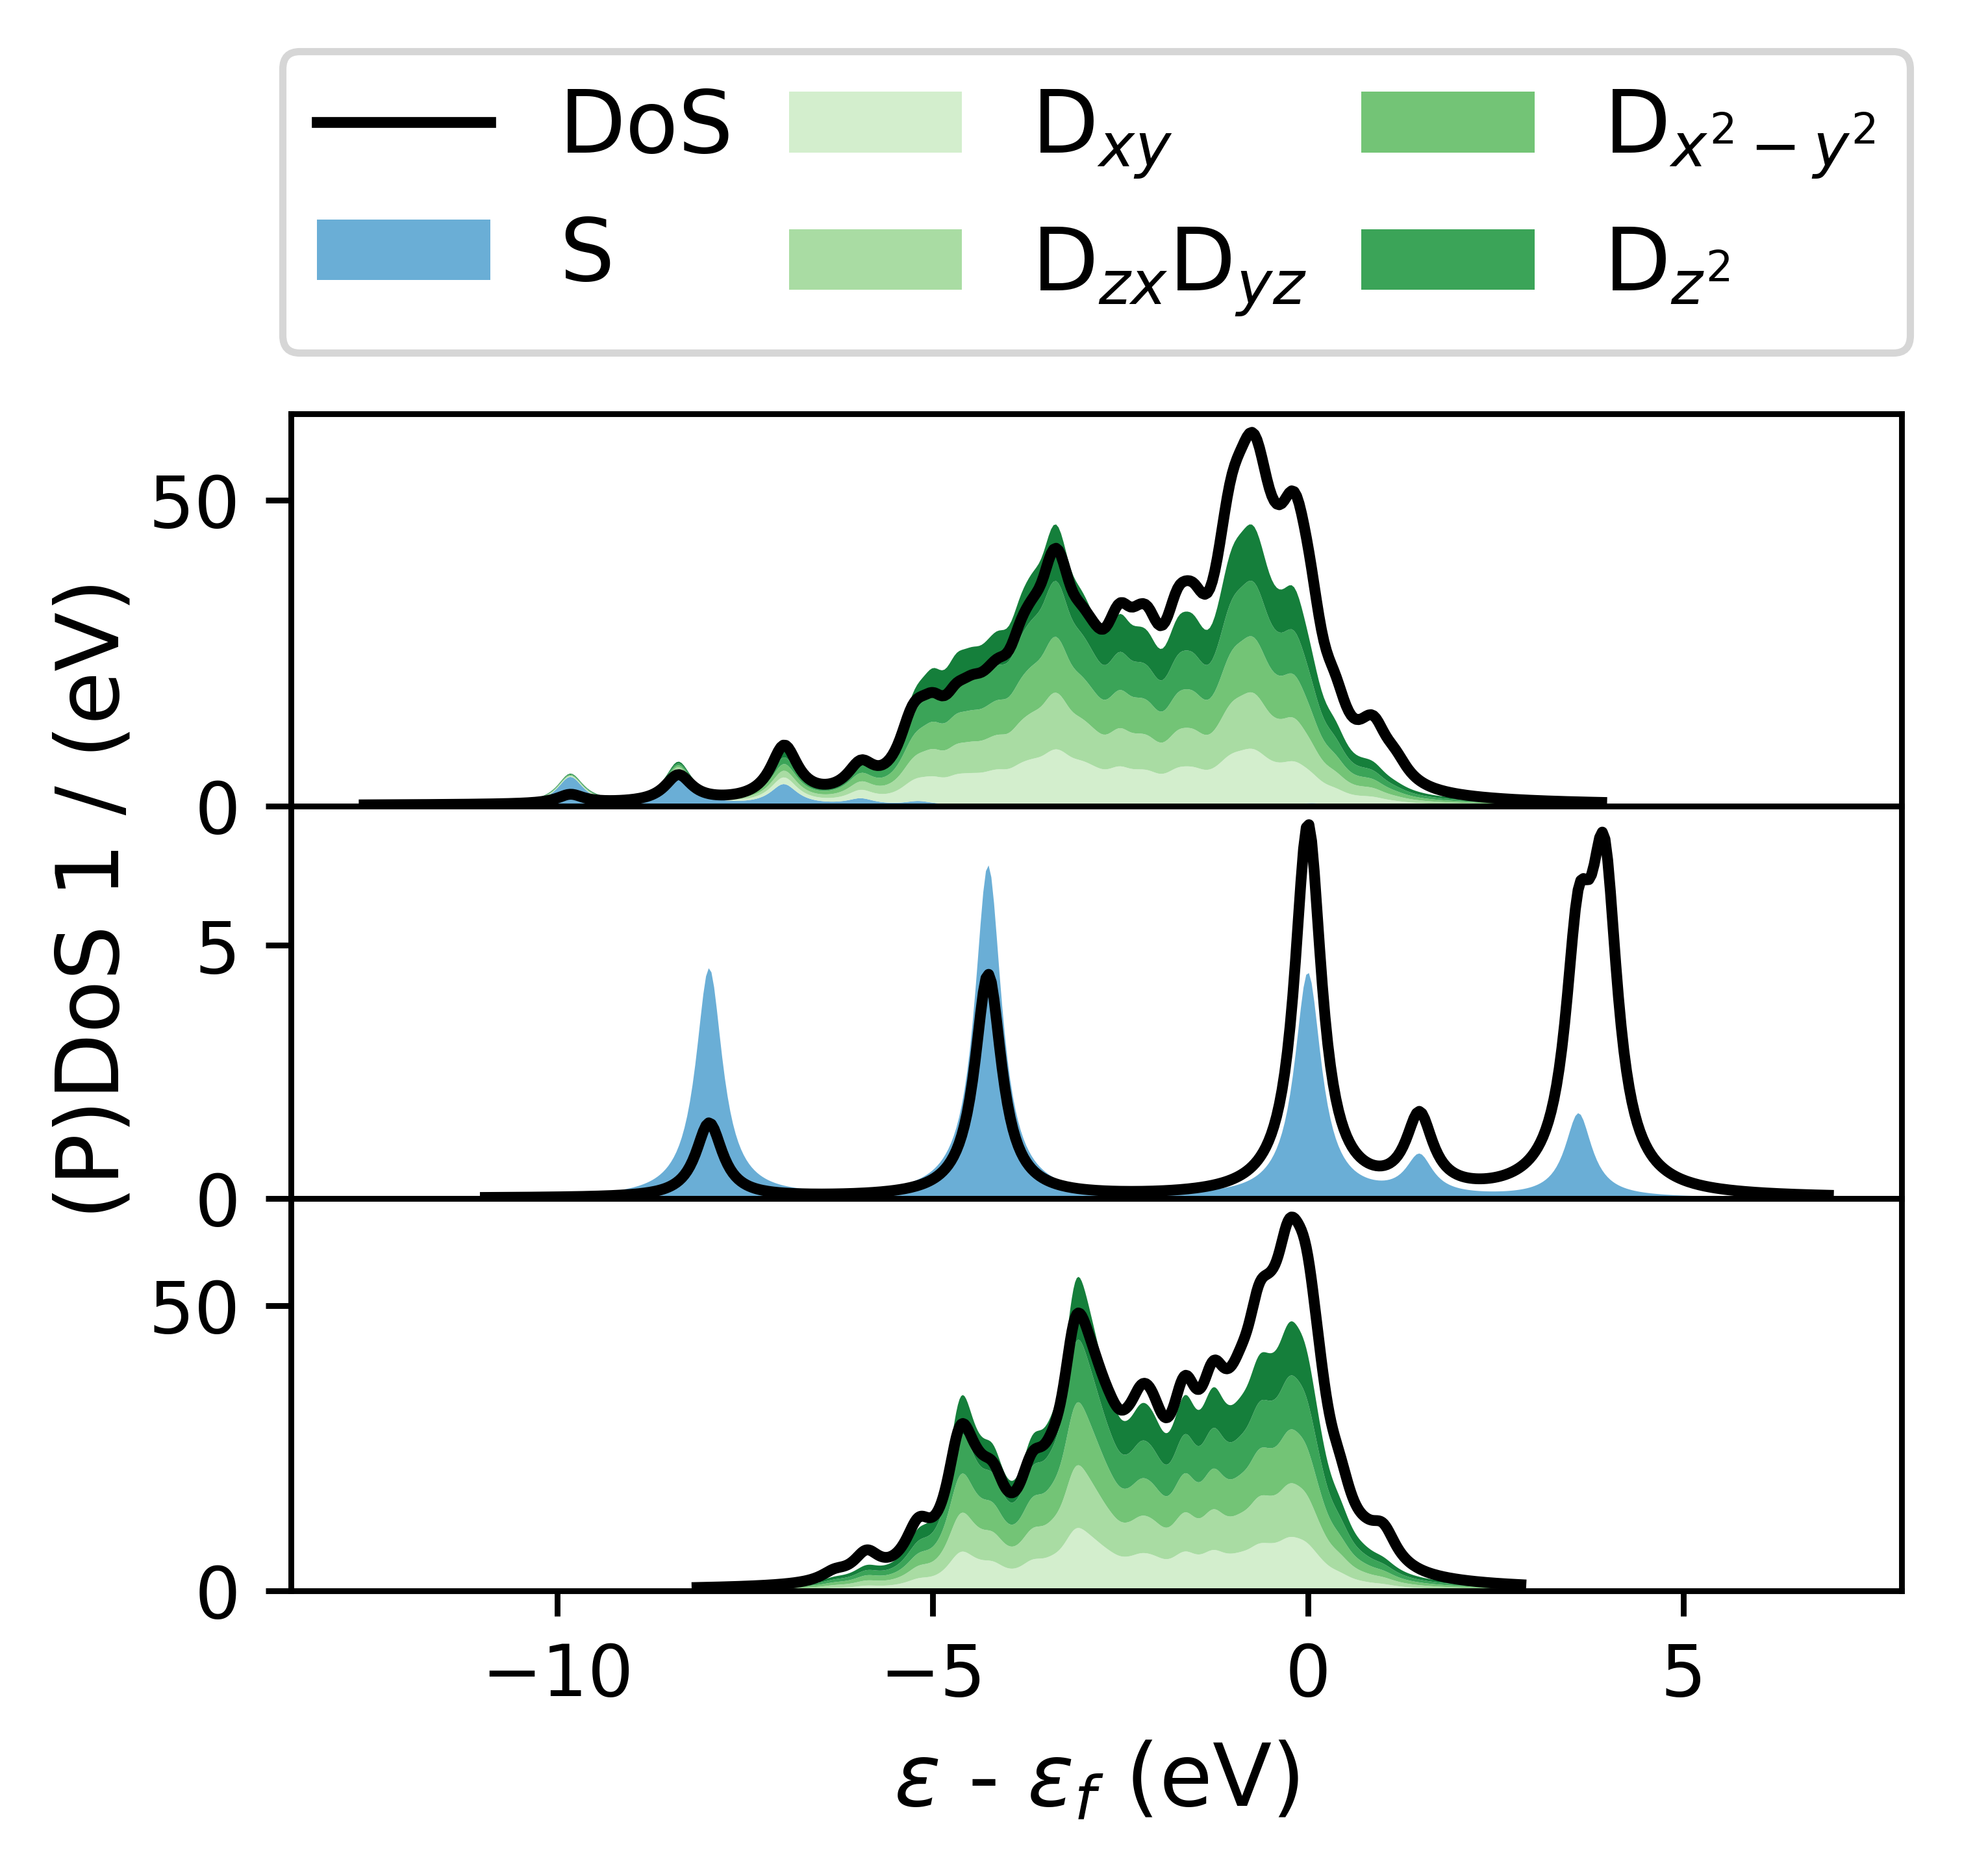
\includegraphics[width=\textwidth]{figures/LM/Atomistic/AuPt_CS_DoS.png}
        \caption{Density of states and projected density of states. Top panel - Au$_{13}^{Ih}$Pt$_{32}^{Shell}$. Middle panel - Au$_{13}^{Ih}$. Bottom panel - Pt$_{42}^{Shell}$.}
        \label{fig:CS_DoS}
    \end{subfigure}
    \begin{subfigure}{0.45\textwidth}
        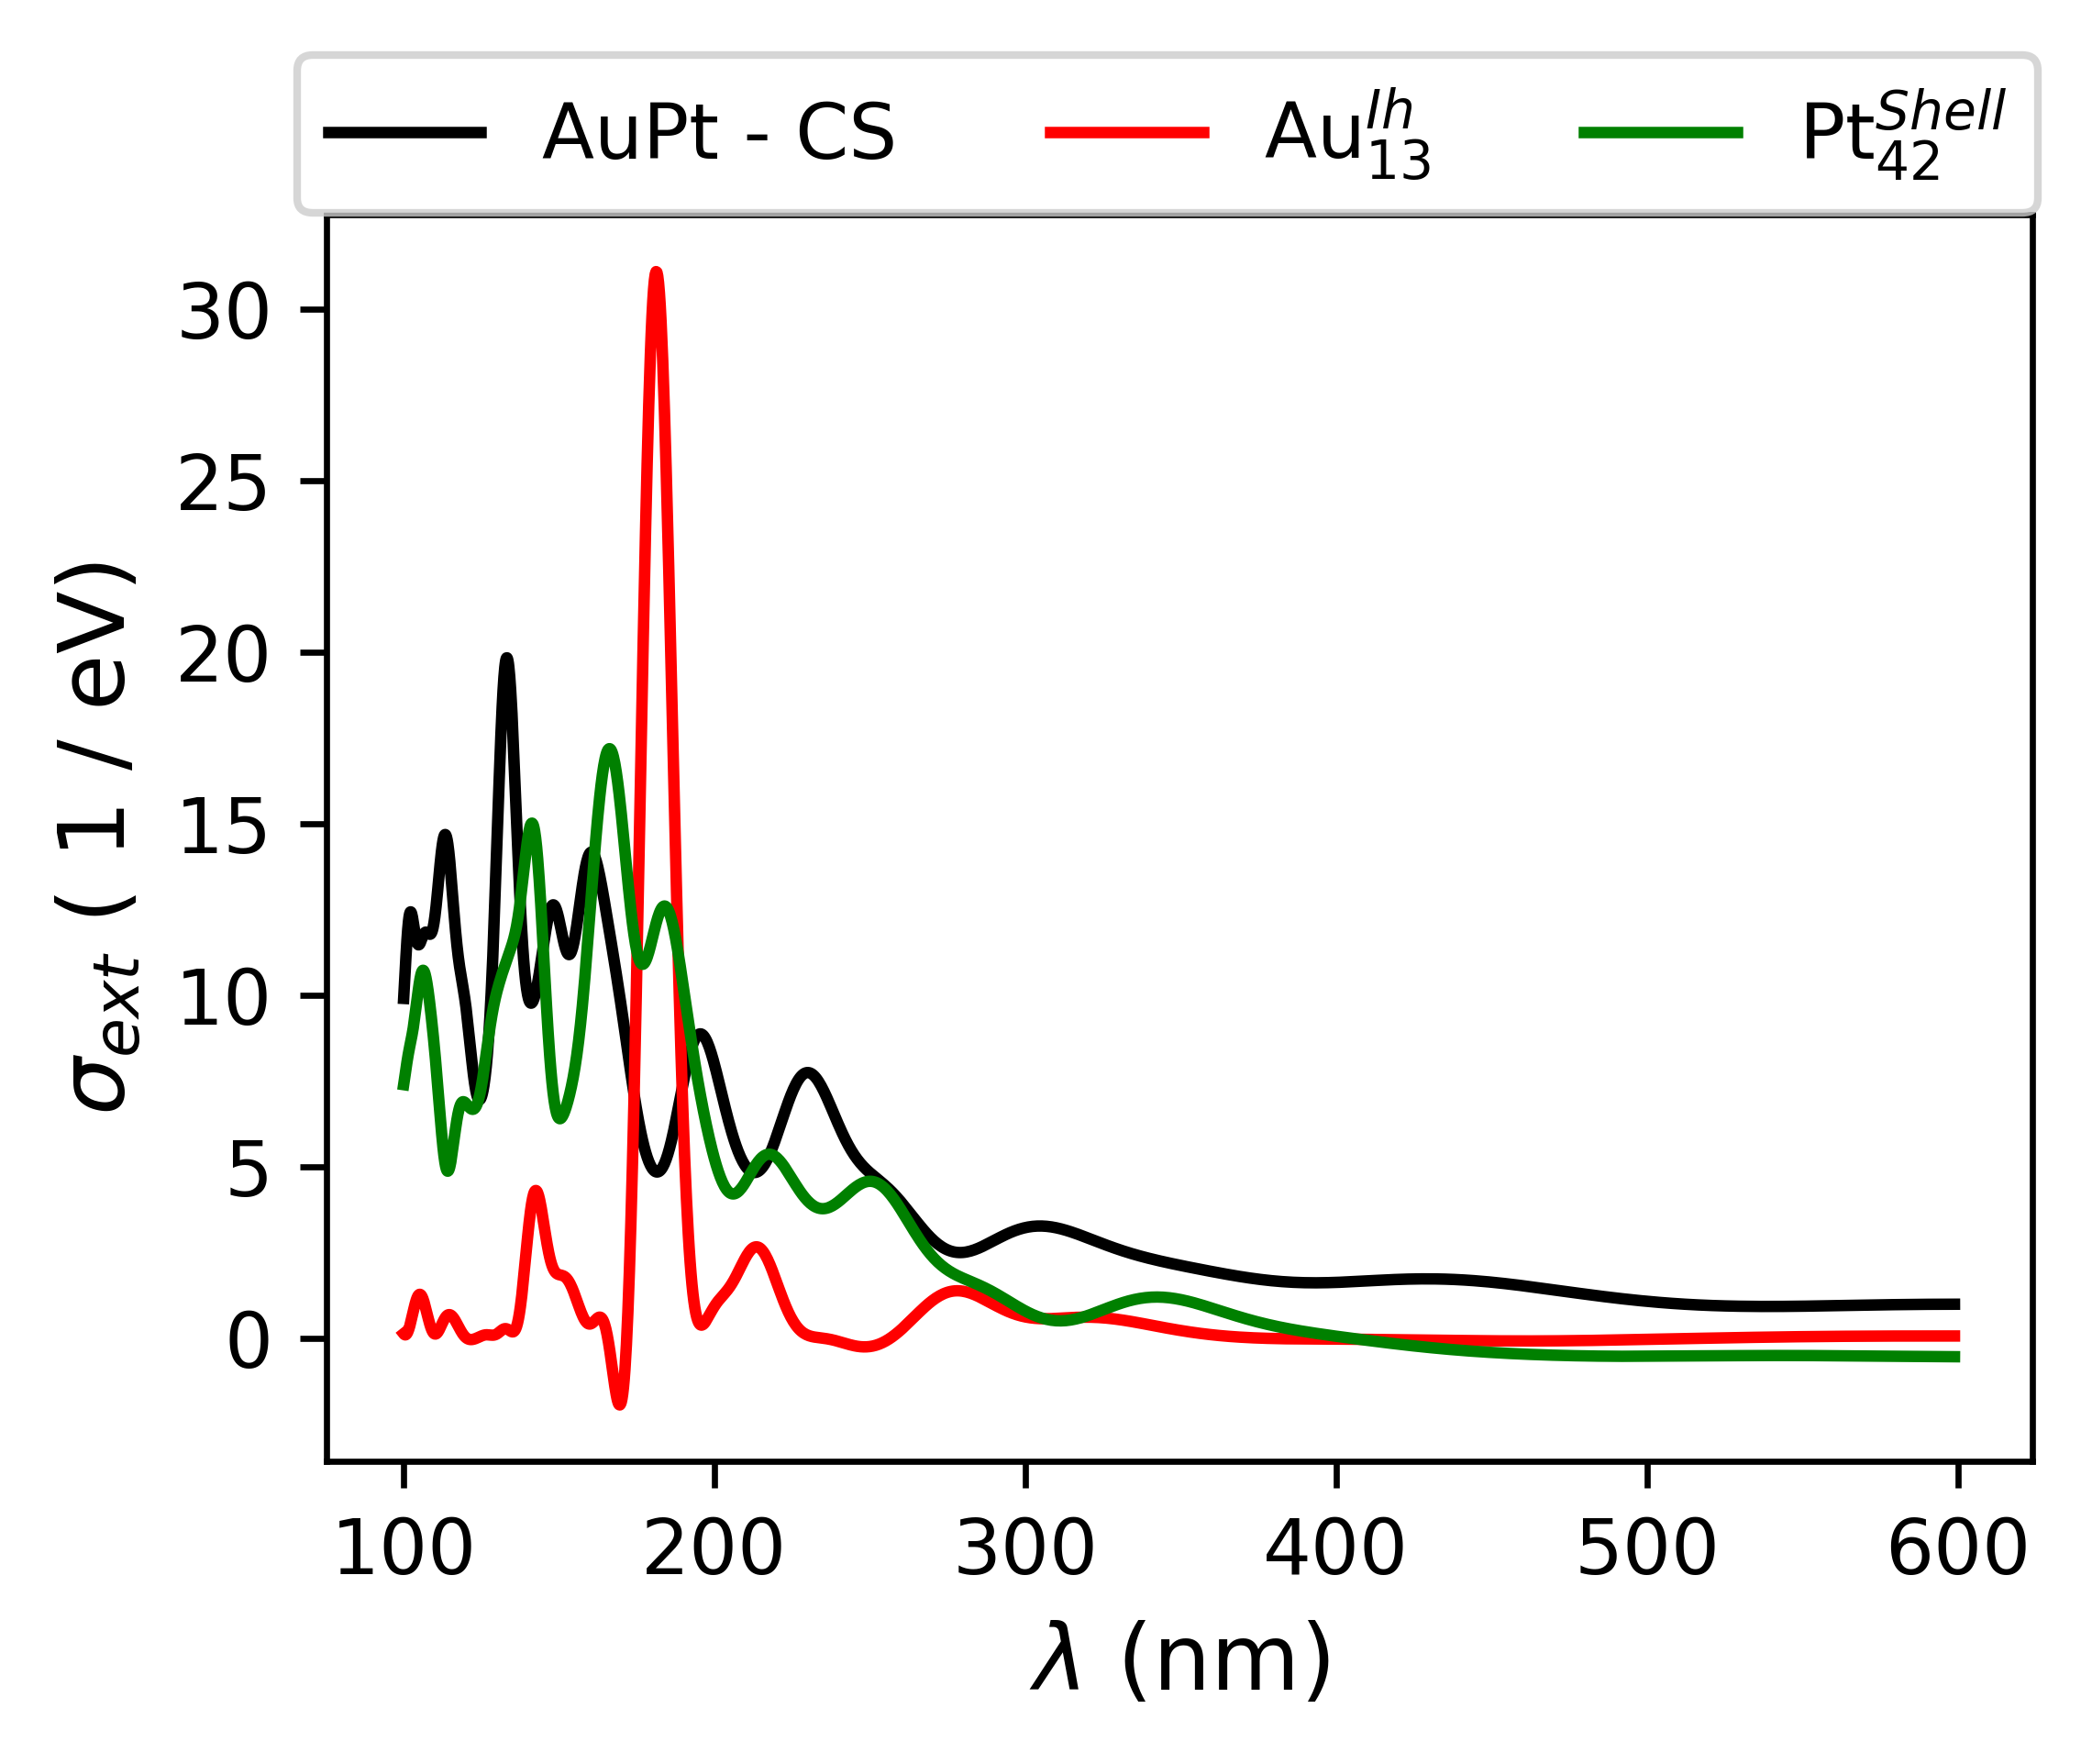
\includegraphics[width=\textwidth]{figures/LM/Atomistic/CS_CSV.png}
        \caption{Extinction spectra for each cluster considered.}
        \label{fig:CS_CSV}
    \end{subfigure}
    \caption{Opto~-~electronic properties for a test Au$_{13}$Pt$_{42}$ - CS test system. (\textbf{a}) Calculated density of states (black) and the orbital resolved projected density of states (blue and green). All calculations performed with the HGH class of pseudopotentials \cite{PhysRevB.58.3641} at the LDA level of theory.}
    \label{fig:DFT_CS}
\end{figure}

We conclude this brief investigation into alloying by considering both the static properties of the clusters from the perspective of the DoS and the projected density of states (PDoS). We first must address the apparent discrepancies with respect to these two descriptions of what in principle should be the same quantity. In \texttt{Octopus} 11.1, the PDoS is computed from the bare pseudo-atomic orbitals, directly taken from the pseudopotentials we have used. The orbitals are not orthonormalised, in order to preserve the character of the atomic orbitals. Consequently, the sum of the different PDoS does not necessarily integrate to the total DoS. Therefore, the shape of the distribution is preserved, if not necessarily what they respectively integrate to. 

Having addressed the first striking feature, we now address the distribution of the 6$s$ orbitals of Au with respect to the bare cluster and at the core of the AuPt NA. It appears that these electron orbitals are redistributed to lower lying states which may account for the lack of optical activity of the AuPt Core-Shell cluster seen in Figure \ref{fig:CS_TD} given that the plasmons are typically associated with either interband transitions from the $d$ to the $sp$ orbitals, or by intraband transitions within $sp$ orbitals. With a lack of available states for such transitions to occur, it is unlikely that such collective motion may be observed. More likely that any observed excitations are the consequence of $d$ to $d$ intraband transitions.

However, we may also observe that there is an appreciable redistribution in the near-HOMO $d$ orbitals of the Core-Shell NA wherein the large collection of orbitals just below the HOMO appears to be splitting into two separate peaks which represents a shift in the $d$-band of the Pt - a crucial concept in catalytic science \cite{Nrskov2011,Nrskov2009,Ruban1997}. However, this property is typically used only to describe periodic structures such as extended surfaces upon which one may undergo catalytic reactions. Nonetheless, there are efforts to reconcile $d$-band centre theory with finite nanoparticle systems \cite{Gorzkowski2015}, though we shall reserve such analyses for a future study and instead acknowledge the incumbent significance. 

Therefore, via the introduction of Au within a Pt shell, we have demonstrated the ability to not only influence the optical character of the Pt by enhancing it with the vibrant response of Au, but we have also influenced the $d$-type orbitals which may have broader consequences from the perspective of catalytic activity. 

Considering now the optical response reported in Figure \ref{fig:CS_CSV}, we first note the sharp peak of Au$_{13}^{Ih}$, as we saw previously in Figure \ref{fig:AuNPs_CSV}, which may be contrasted against the more chaotic landscape of the absorption spectrum for Pt$_{42}^{Shell}$. However, what we are truly interested in is the effect that the alloying has had on this property, in that we may see that two new peaks emerge in the spectrum for the Core-Shell cluster at approximately $\pm$50 nm either side of the sharp Au peak. Moreover, we observe that the peak visible for Pt$_{42}^{Shell}$ at $\sim$ 190 nm, and was congruent with that of Au appears to have been suppressed -  a consequence of the alloying.

Given the simplicity of the LDA pseudopotentials used, we shall conduct a more comprehensive analysis of the alloying of Au and Pt within the \textit{ab initio} regime by using the FHI pseudopotentials which feature the $d$ orbitals of Au so that we may be more precise in our analysis of the effect that this alloying may have on the $d$ orbitals of Pt. Moreover, as observed in Figure \ref{fig:pps}, there are indeed more nuances in the exitniction spectrum of Au when more electrons are explicitly considered which should make for a richer investigation.

\subsection{Jellium model for Au nanoparticles}
\label{sec:Res_JLM}

\begin{figure}[ht!]
    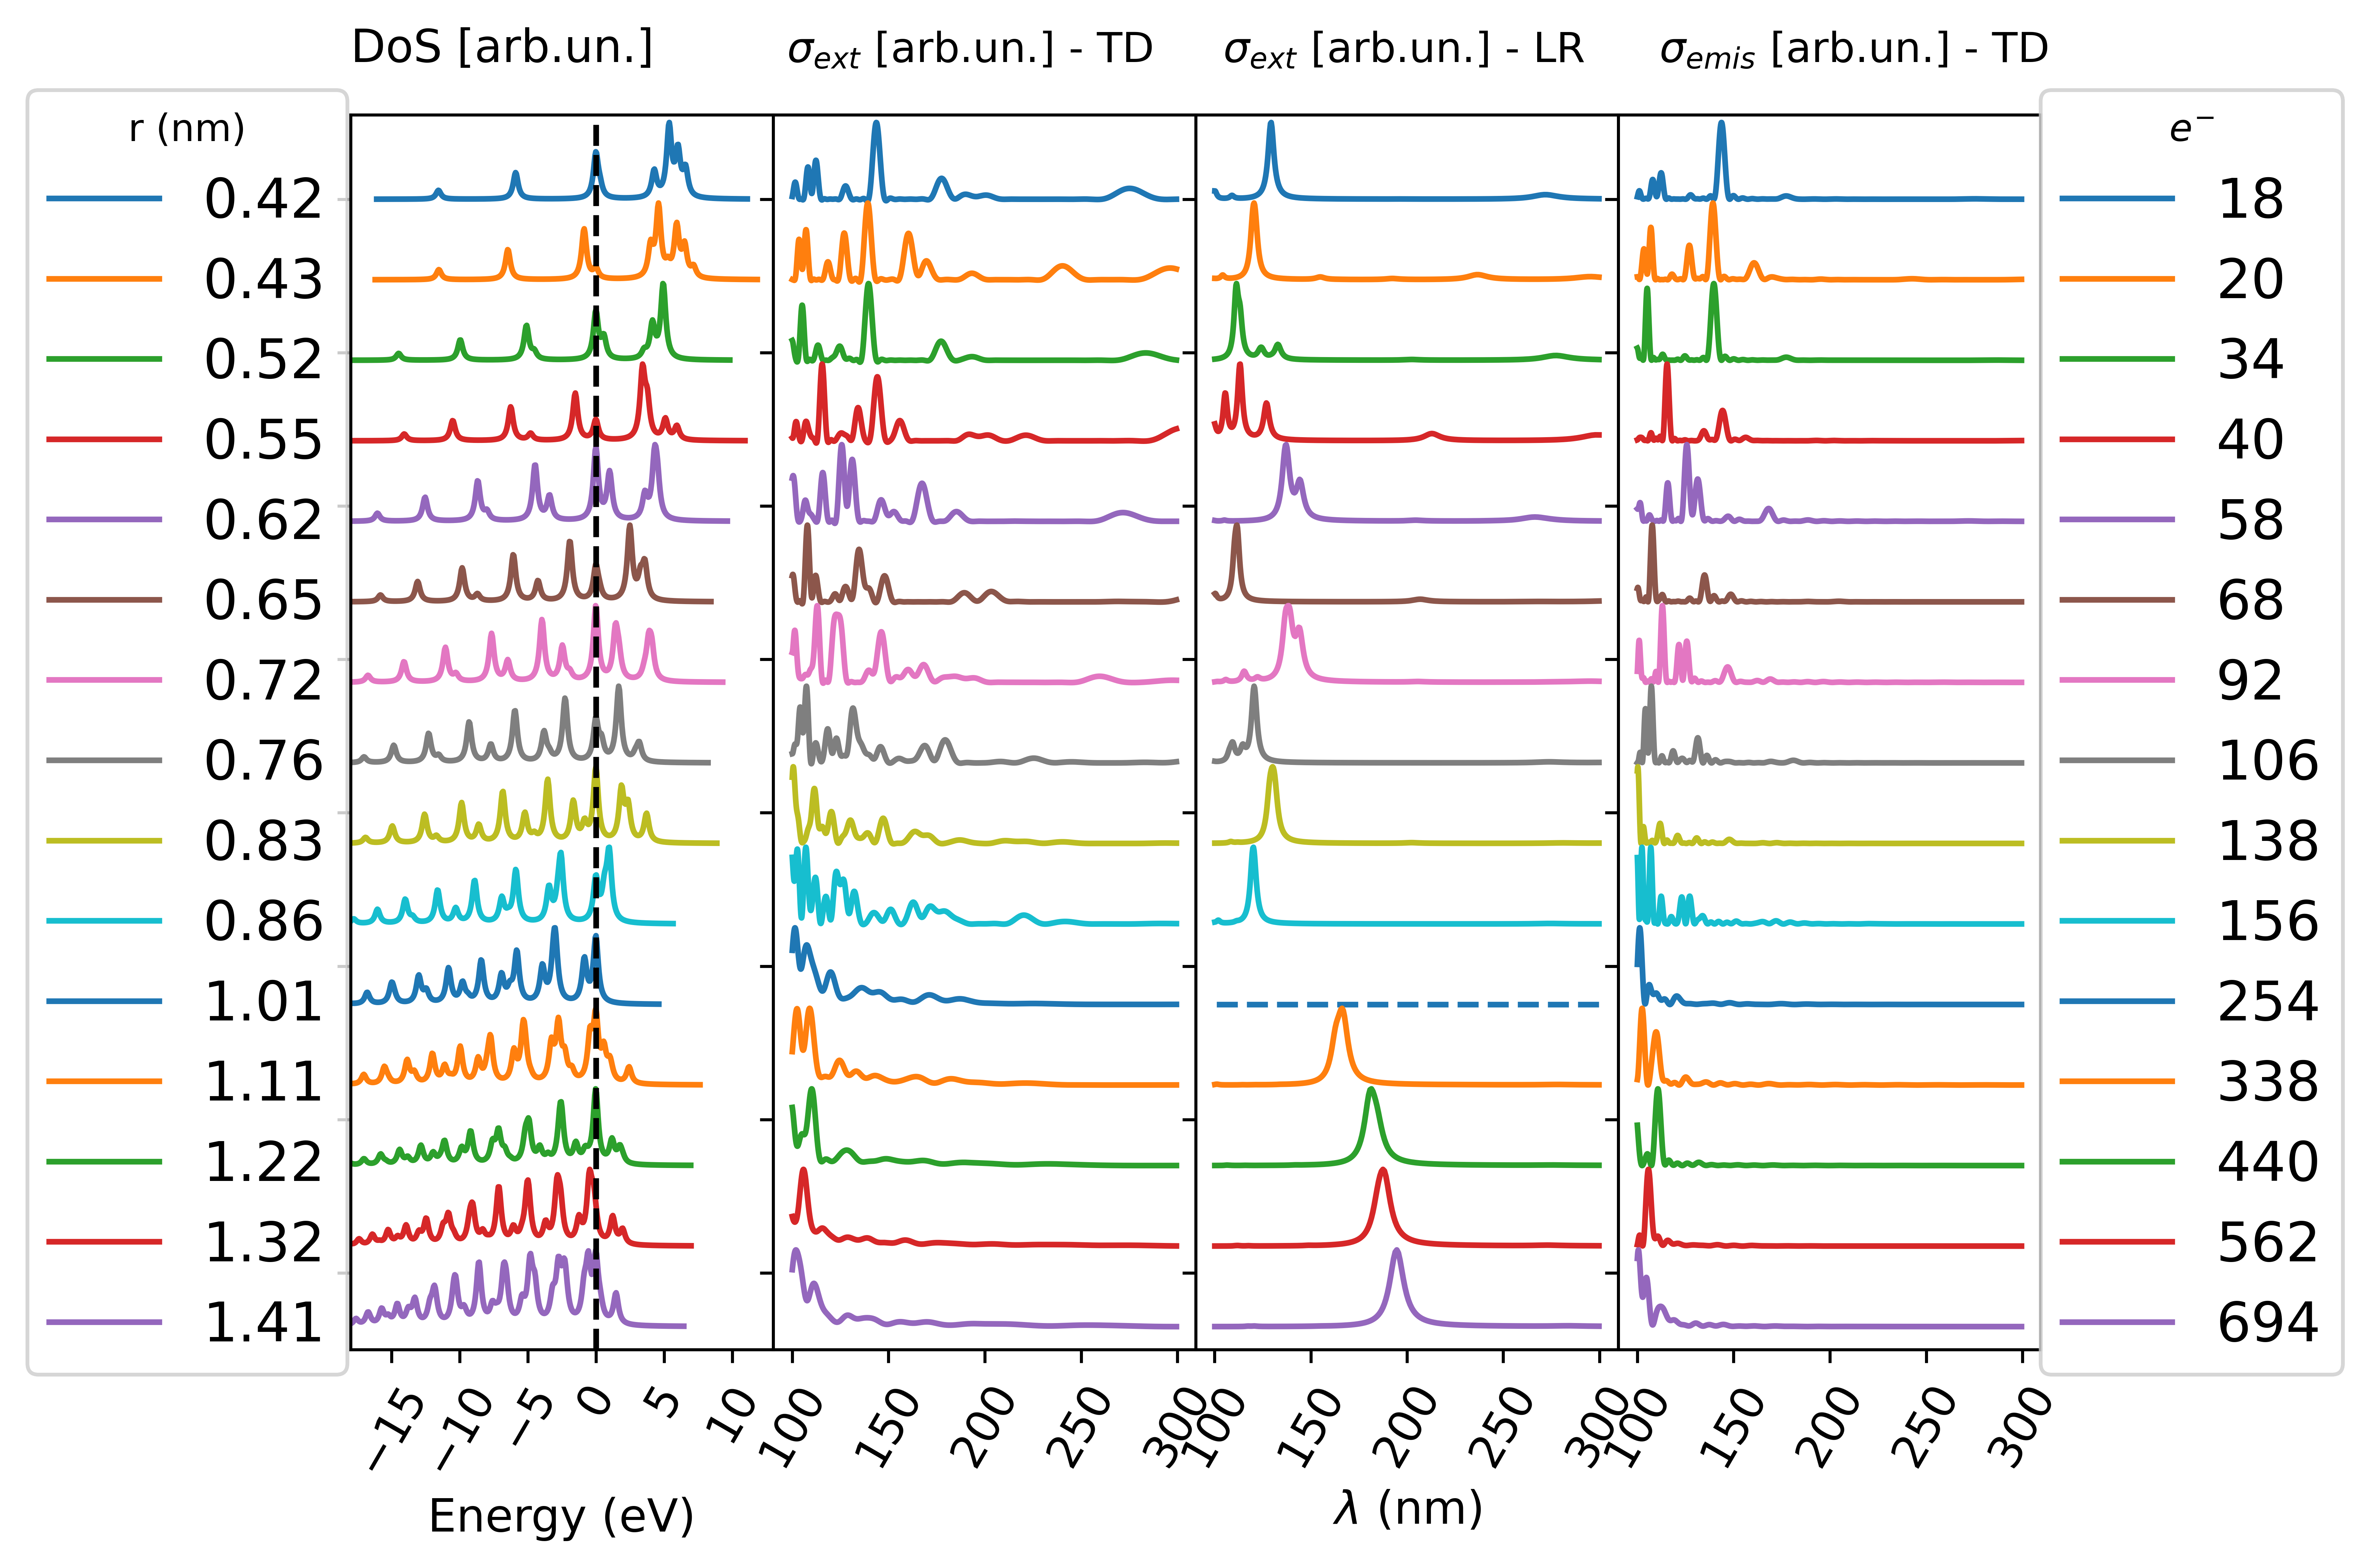
\includegraphics[width=0.9\textwidth]{figures/LM/JLM/Sizes_Jlm.png}
    \caption{Varying the number of electrons in the Jellium (different colours) corresponding to electronic closure cases. Left hand is DoS vs energy and the dashed line refers to the HOMO in \texttt{Octopus}. Centre-left is the absorption spectrum computed via the TDDFT $\delta$-kick method. Centre-right is the Casida spectrum with 20 empty states. Right column is the harmonic spectrum computed via Equation \ref{eqn:HHG}. Dashed lines indicate a failure to converge to calculation.}
    \label{Fig:Jlm_Sizes}
\end{figure}

By considering the size dependence of the Jellium model in Figure \ref{Fig:Jlm_Sizes}, we may conclude that there is evidence of a blue-shift in the optical properties as the size is decreased which is indeed predicted for plasmonic materials as described in Section \ref{sec:plasmons}. However, what is interesting to note is the general lack of agreement with respect to the LR treatment of the spectrum against the TDDFT approaches. It is possible that this may be due to numerical complications arising from the dynamics. However, given the time increment of $\sim$ 0.02 attoseconds and a total propagation time of $\sim$ 17 femtoseconds, this is unlikely as these respectively correspond to a tolerance of $\sim$ 60 nm sampling windows and a maximum wavelength of $\sim$ 100 $\mu m$. Whilst this window is not exactly small, it appears sufficient to isolate fine details in both the extinction spectrum and harmonic spectrum computed via the TDDFT method given the appearance of the plots. It is possible that the lack of high energy peaks in the Casida spectra are due to the number of empty states considered, or lack thereof. Whilst we have used 20 states uniformly for each cluster, it is clear from the depiction of the DoS in the left column of Figure \ref{Fig:Jlm_Sizes} that for larger structures this is an insufficient number to adequately describe these high energy excitations.

Given that the maximum energy considered above the HOMO states are offset by $\sim$ 5 eV, which corresponds to $\sim$ 200 nm, it seems likely that is the cause of disagreement between the results with respect to the high energy excitations in the Casida approach \cite{Casida}. However, it does not disculpate the lack of low energy excitations visible in the spectra derived from TDDFT. It may simply be that during the numerical convolution of the spectrum, the size intensity of the high energy peaks drowns out the signal in the lower energy regions as any issue regarding the conversion of numerical parameters should only affect the high energy regions. For example, the tightness of the real space grid mesh essentially governs the energy cutoff when compared with k-space DFT methods \cite{cp2k_2020}. Therefore, one may intuit that if the high energy regions are sufficiently converged, so too should the low energy regions. Here, however, is the caveat. We assume that these high energy regions \textit{are} sufficiently converged. We consider this unlikely as there is a general agreement in the shape of the high energy region for all of the considered Jellium clusters. Indeed, it is far more likely that these are indeed represented in these spectra, but are smoothed over due to the Lorentzian broadening occurring on the large volume of high energy delta points in the spectrum. 

Indeed, we have demonstrated that the seemingly simple task of computing optical spectra for small Jellium clusters is a non-trivial task that requires careful consideration of both the input parameters for the calculations and indeed the parameters for the post-processing of the output. In the following works, we are sapient to these pitfalls and ensure that we are sufficiently sensitive to the aforementioned considerations. Moreover, due to the poor scaling of the Casida method \cite{Casida}, we generally shall not report further these spectra. Whilst this method is exact in the limit of an infinite number of unoccupied states, the rate at which the computational cost grows is necessarily factorial in the total number of states where the number of unoccupied states must grow too with system size to adequately probe the higher energy excitations. 

As discussed in the previous section, the laser function in \texttt{Octopus} is a remarkable tool for simulating more realistic light-matter interactions with tunable functionality. Given the numerical inconsistencies with the numerical approach to evolving individual atoms at the time of writing this thesis, we shall instead discuss the scope of how such laser profiles may be introduced once the implementation reaches maturity. In future investigations, we wish to utilise this laser feature to more directly emulate the procedure of a pump probe experiment. Given that within \texttt{Octopus} one may create a series of laser profiles such that a large near-resonant laser may be incident upon the desired sample who is then permitted to evolve under their own electron dynamics for a sufficiently long period for the oscillations in the dipole moment to approach coherency. After $\sim$ 100 femtoseconds of unperturbed dynamics, a second off-resonance laser pulse may be incident orthogonal to the pumping laser as is common practice in experimental procedures \cite{https://doi.org/10.1002/lpor.202000346}. Indeed, it is feasible at the theory level of the LDA to compute hot carrier lifetimes from such dynamics \cite{https://doi.org/10.1002/lpor.202000346}, doing so unfortunately remains beyond the scope of this project whose true purpose has been to determine what is feasible with respect to introducing laser excitations into nanosystems. 

Finally worthy of note and reflection is that the Jellium model, in principle, has perfect spherical symmetry in that it is by construction homogeneous, uniform, and isotropic \cite{Jellium}. Therefore, we anticipate that this model may exhibit closer agreement with the more richly symmetric Au MNPs described in Figure \ref{fig:DFT_AuNPs} and Table \ref{tab:symmetry_groups}. With respect to the DoS reported in both instances, we do indeed see this type of agreement, where there is evidence of structure which may be a consequence of the symmetries present. Conversely, the absorption spectra computed from real~-~time propagation have share much poorer resemblance. As has been discussed, this may be a consequence of the numerical limitations of using the Jellium model for smaller clusters as the structure in the absorption spectra from both the Caisida and real~-~time propagation methods appears to be recovered at larger cluster sizes. Nonetheless, there is sufficient evidence between these classes of calculations to conclude that the existence and richness of symmetries within MNPs appears to influence both the DoS and optical spectra of such systems ~-~ in agreement with previous studies \cite{doi:10.1021/acs.jpca.8b07923}.

\section{Effect of structural changes: the breathing of gold cages}
\label{Pure}

We show in the article of Zhao \textit{et al} \cite{Wei} that optical properties change when the fullerene structures of Au$_{32}$, Cu$_{32}$ and Ag$_{32}$ inflate and deflate. We first observe significant differences in the extinction spectra employing a classical approach based on the Green's dyadic method. By means of real-time time-dependent density functional theory, we continue to calculate the optical spectrum via a $\delta$-kick simulation, comparing results with the ground-state energetic property with the HOMO-LUMO gap. However, these subsequent results are not the original work of the author and so will only be discussed in the appropriate context.

Inspired by experimental observations \cite{Maioli2018,Quasi_Breathe}, we investigate how a radial breathing mode might alter the physical properties of the highly symmetric and spherical fullerene cage. We consider both deflation and inflation of the cage. Whilst we expect that different isomers will show different optical spectra, we are solely investigating the effect of small structural changes not altering the shape or the symmetry of the cluster morphology. One can expect that a similar motion might take place at finite temperatures, further showing the strong coupling between vibration and optical properties in small clusters \cite{Liu2021}. Quite surprisingly, we found that even small radial changes affect drastically the electronic and optical properties of noble metal cages. We calculate the optical spectra of fullerene cages of Au, Cu, and Ag at 32 atoms by means of real-time time-dependent density functional theory (RT-TDDFT) and perform comparisons between this \textit{ab initio} TDDFT method and a classical coupled dipole approximation \cite{Ullrich2012}. In doing so, we intend to identify how the quantum mechanical properties of small metallic clusters will result in deviations from a classical electrostatic consideration. We analyse the energetic, electronic, and optical properties of radially inflated and deflated cages, using a dimensionless parameter $\gamma$ to denote the radial compression/dilatation of up to 12\%.
While Au and Cu present some similarities, for example, in the main changes between inflated and deflated cages, Ag shows a monotonic red-shift of the the first peak of the optical absorption in the visible frequencies. We contrast the change of the position of the first peak in the optical spectra of Au$_{32}$, Cu$_{32}$, and Ag$_{32}$ with the HOMO-LUMO gap showing that they are not simply related.

\begin{figure}
\centering
\begin{subfigure}[b]{0.6\textwidth}
    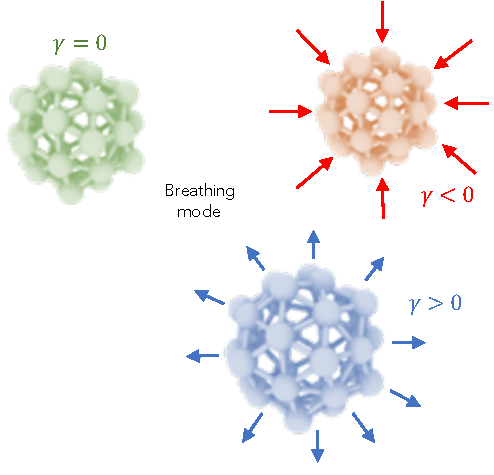
\includegraphics[width=\textwidth]{figures/LM/GDM/Strut_breathingmode.pdf}
    \caption{} 
    \label{Fig:Breathe_Modes}
\end{subfigure}
\begin{subfigure}[b]{0.35\textwidth}
    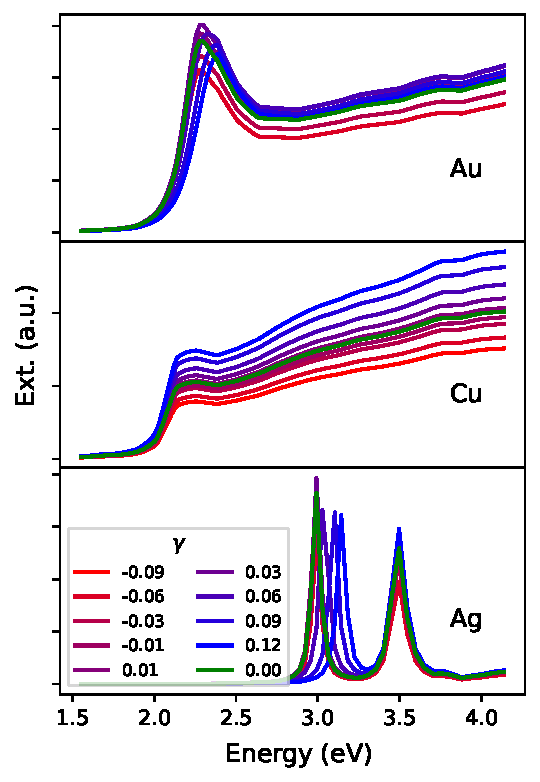
\includegraphics[width=\textwidth]{figures/LM/GDM/ClassicalSpectra_Smol.pdf}
    \caption{}
    \label{Fig:Breathe_Spectra}
    \end{subfigure}
    \caption{Illustration of how the induced breathing of metallic fullerene cages (\textbf{a}) influences the classically calculated optical extinction spectrum (\textbf{b}) as a function of the breathing parameter $\gamma$. Reprinted with permission from IOP Science Journal of Physics: Condensed Matter, Volume 34, Number 22 \cite{Wei}.}
    \label{Fig:Breathe}
\end{figure}

The fullerene cages with 32 atoms for pure gold, copper, and silver are shown in Figure \ref{Fig:Breathe_Modes}. This cage is obtained removing the inner core of an anti-Mackay Ih with 42 atoms and it has been shown to be the dual of the most famous C$_{60}$ molecule \cite{Trombach2016}. This breathing mode is mechanically mimicked by inflating and deflating the cage in a similar fashion to a balloon. In practice, this is achieved by numerically adjusting the average distance of each atom from the centre of mass by radially displacing the atoms by a specified amount, depending on the desired breathing coefficient $\gamma$, introduced as
\begin{equation}
    \gamma=\frac{R_{COM}}{R_{0}}-1,
\end{equation}
where $R_{COM}$ and $R_0$ represent the average radial distance of the metallic atoms from the centre of mass for the structure, and the ionically relaxed case, respectively. Under this notation, the relaxed stable gold, copper, and silver fullerene correspond to a vanishing breathing coefficient $\gamma$. A deflation is identified by a negative breathing coefficient, whereas the inflated shapes have a positive breathing coefficient. We thoroughly examined the structures with $\gamma$ between -0.09 and 0.12. In the article, we proceed to demonstrate, via arguments of energetic stability, we do expect that such a breathing mode can take place at finite temperatures. Nonetheless, we are able to show how relatively small structural changes influence the optical properties, and indeed the electronic properties in the reference paper.

We remark before presenting results that the primary purpose of this investigation was not to explicitly compute these fundamental breathing modes themselves, as has been studied at length \cite{doi:10.1021/jp014068s,PhysRevB.80.035411,doi:10.1021/jp051575r}. Rather, assuming that such a mode exists, we ask the question of ``Will optical properties be influenced by a nanoparticle `breathing'?'' Indeed, the structures in this section do not necessarily represent local minima in their respective PES landscapes, but are designed as caricatures of instantaneous states during the breathing process. 

First, let us discuss the extinction spectra of breathing fullerene cages, Figure \ref{Fig:Breathe_Spectra}. We note that the three metals have different behaviour where Au and Cu mainly changing the intensity of their peak well positioned in the visible region. In this respect, Au clusters have just one peak around 2.2 eV, which mildly blue-shift for large and positive $\gamma$. However, Cu shows a monotonic change of the intensity as we move from negative to positive values of the breathing parameter. Finally, Ag cages show two clear peaks. The one at higher energies, approximately 3.5 eV, is almost independent from the breathing parameter (its intensity slowly grows with $\gamma$), while the one at lower energy shows a dramatic dependence on $\gamma$, with a significant blue-shift of its position for inflated cages. It is sufficiently self-evident, even at a classical level as one may observe in Figure \ref{Fig:Breathe_Spectra}, that during the breathing of a hollow cage we observe changes in the optical properties. However, these variations suffer from the same crude approximations acknowledged in Sec. \ref{sec:GDM}, that is to say that we do not explicitly take into account the interactions between the electrons. With that said, Figure \ref{Fig:Breathe_Spectra} demonstrates the necessity in acknowledging the stimulated variation in extinction spectrum when a nanoparticle is instantaneously illuminated. Moreover, one may appreciate that for larger hollow cage-like structures, the classical spectra displayed in Figure \ref{Fig:Breathe_Spectra} will become more representative. Indeed, we shall demonstrate and discuss this precise property in due course of this chapter.

Furthermore, it is worth noting in Figure \ref{Fig:Breathe_Spectra} that the larger structures (due to radial expansion) appear to universally exhibit higher energy absorption peaks relative to the smaller structures. This is in conflict with the assertions made regarding the relationship between the radius of the nanoparticle and its plasma frequency in Section \ref{sec:class_plasma}. In summary, a smaller radius means that there is a stronger restoring force acting on the induced dipole which means that a higher energy photon is required to achieve resonance. In this work, we appear to have found the opposite behaviour. This may be a limitation of the GDM we have used, as the number of elements remains the same whereas their spatial distribution has changed. Nonetheless, this discrepancy merits further attention which we shall explore in the next section.

\section{Atomistic GDM Model}

To critically evaluate the efficacy of the GDM model, we consider several isolated test cases for several metallic species which shall be appearing later in this thesis in greater detail. We isolate our investigations to the morphologies described in Figures \ref{Fig:nanoparticles_sizes} and \ref{fig:struts_example} so as to be consistent with our prior work. Indeed, given the unamicable scaling of the calculations with respect to the number of interacting dipoles, we have considered clusters with fewer than 3000 atoms or approximately 4 to 5 nm in diameter. Small, but not unheard of in experimental communities \cite{JorgeStructure}.  

We are interested in observing the similarity with respect to experimental measurements and the dependence of the extinction cross section on the size and morphology. For reasons discussed in Sec. \ref{sec:GDM}, we do not anticipate large deviations from experimentally observed signals, as the input parameters for this model are explicitly derived from experiment \cite{pyGDM}. However, what is not trivial is the role that morphology and size may play. Intuitively, we expect the intensity of the extinction profile to scale with the area or approximately $n^{2/3}$ as there is an increased amount of exposed surface area of the nanoparticle to absorb and scatter incoming light. Moreover, given that there exist exotic morphologies within our menagerie, it is possible that extended surface features observed in structures such as the Ih, Oh, and MDh may act like nano-antennae - intensifying the near field enhancement around the nanoparticle.

\begin{figure}[b]
    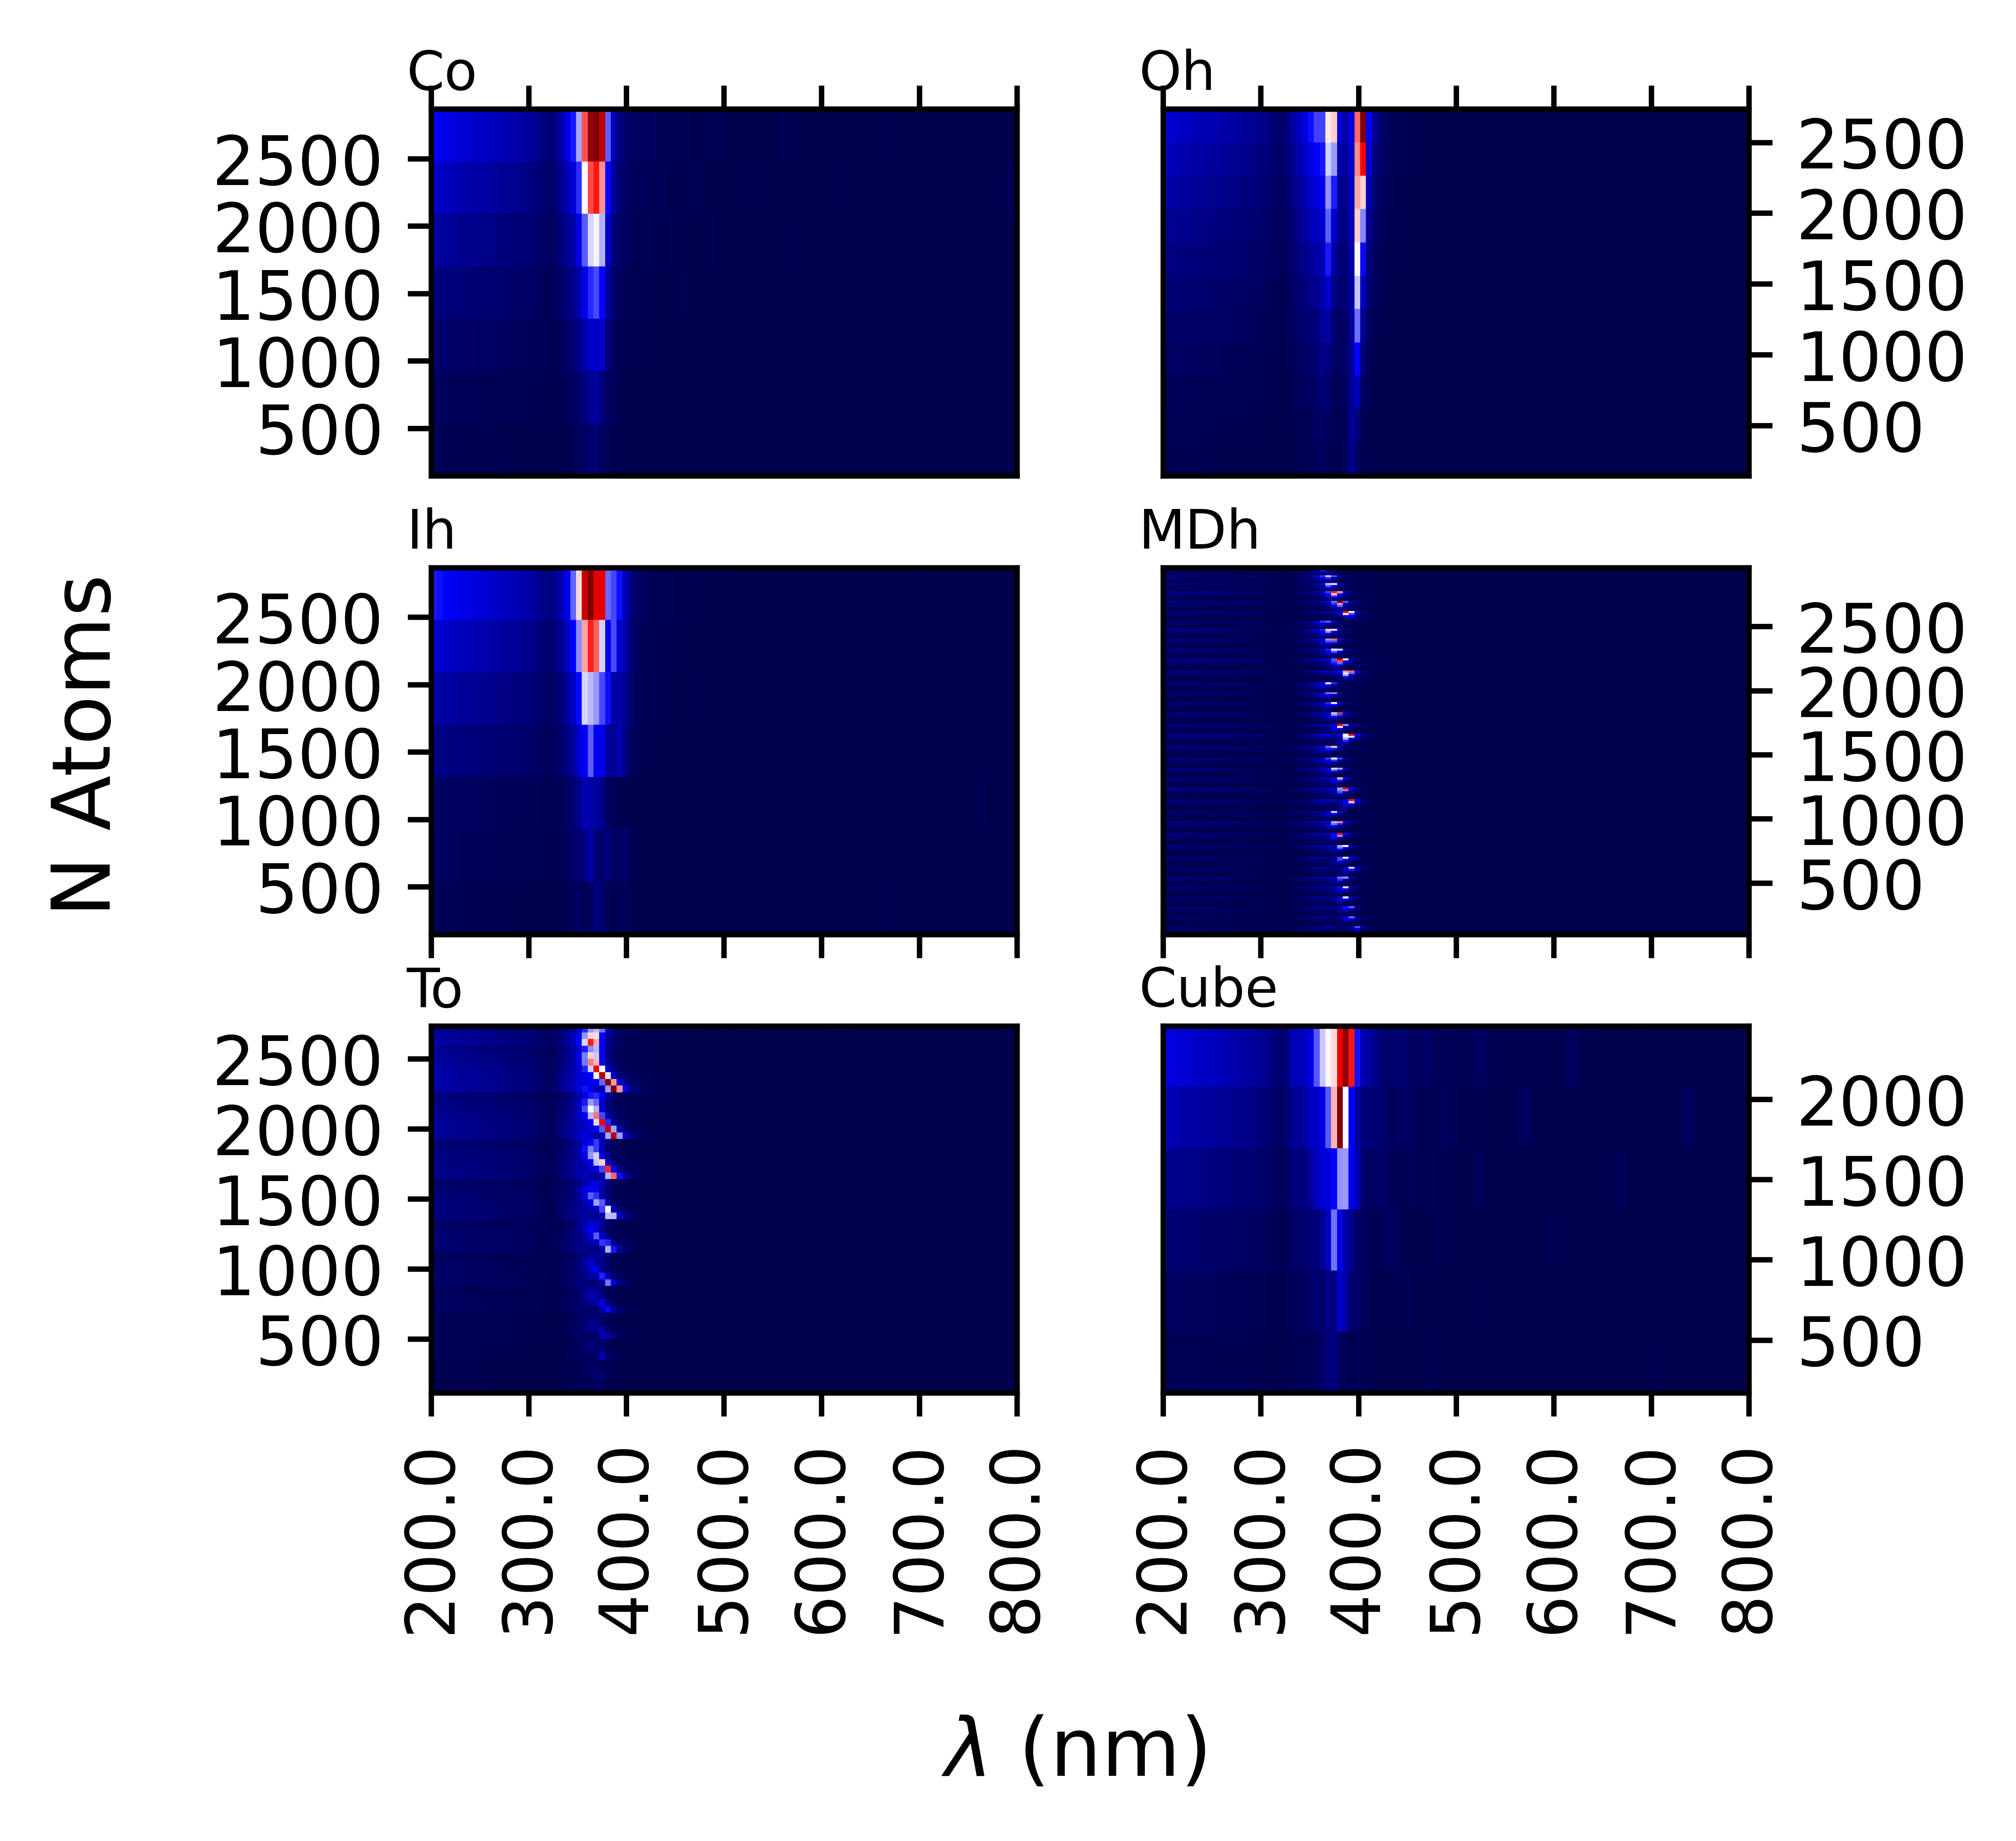
\includegraphics[width=0.95\textwidth]{figures/LM/GDM/Ag_Specs.png}
    \caption{Extinction spectra of varied size and morphology for Ag clusters. Structures considered are a subset of those introduced in Figure \ref{Fig:nanoparticles_sizes}.} 
    \label{Fig:Size_Ag_GDM}
\end{figure}

\begin{figure}[b]
    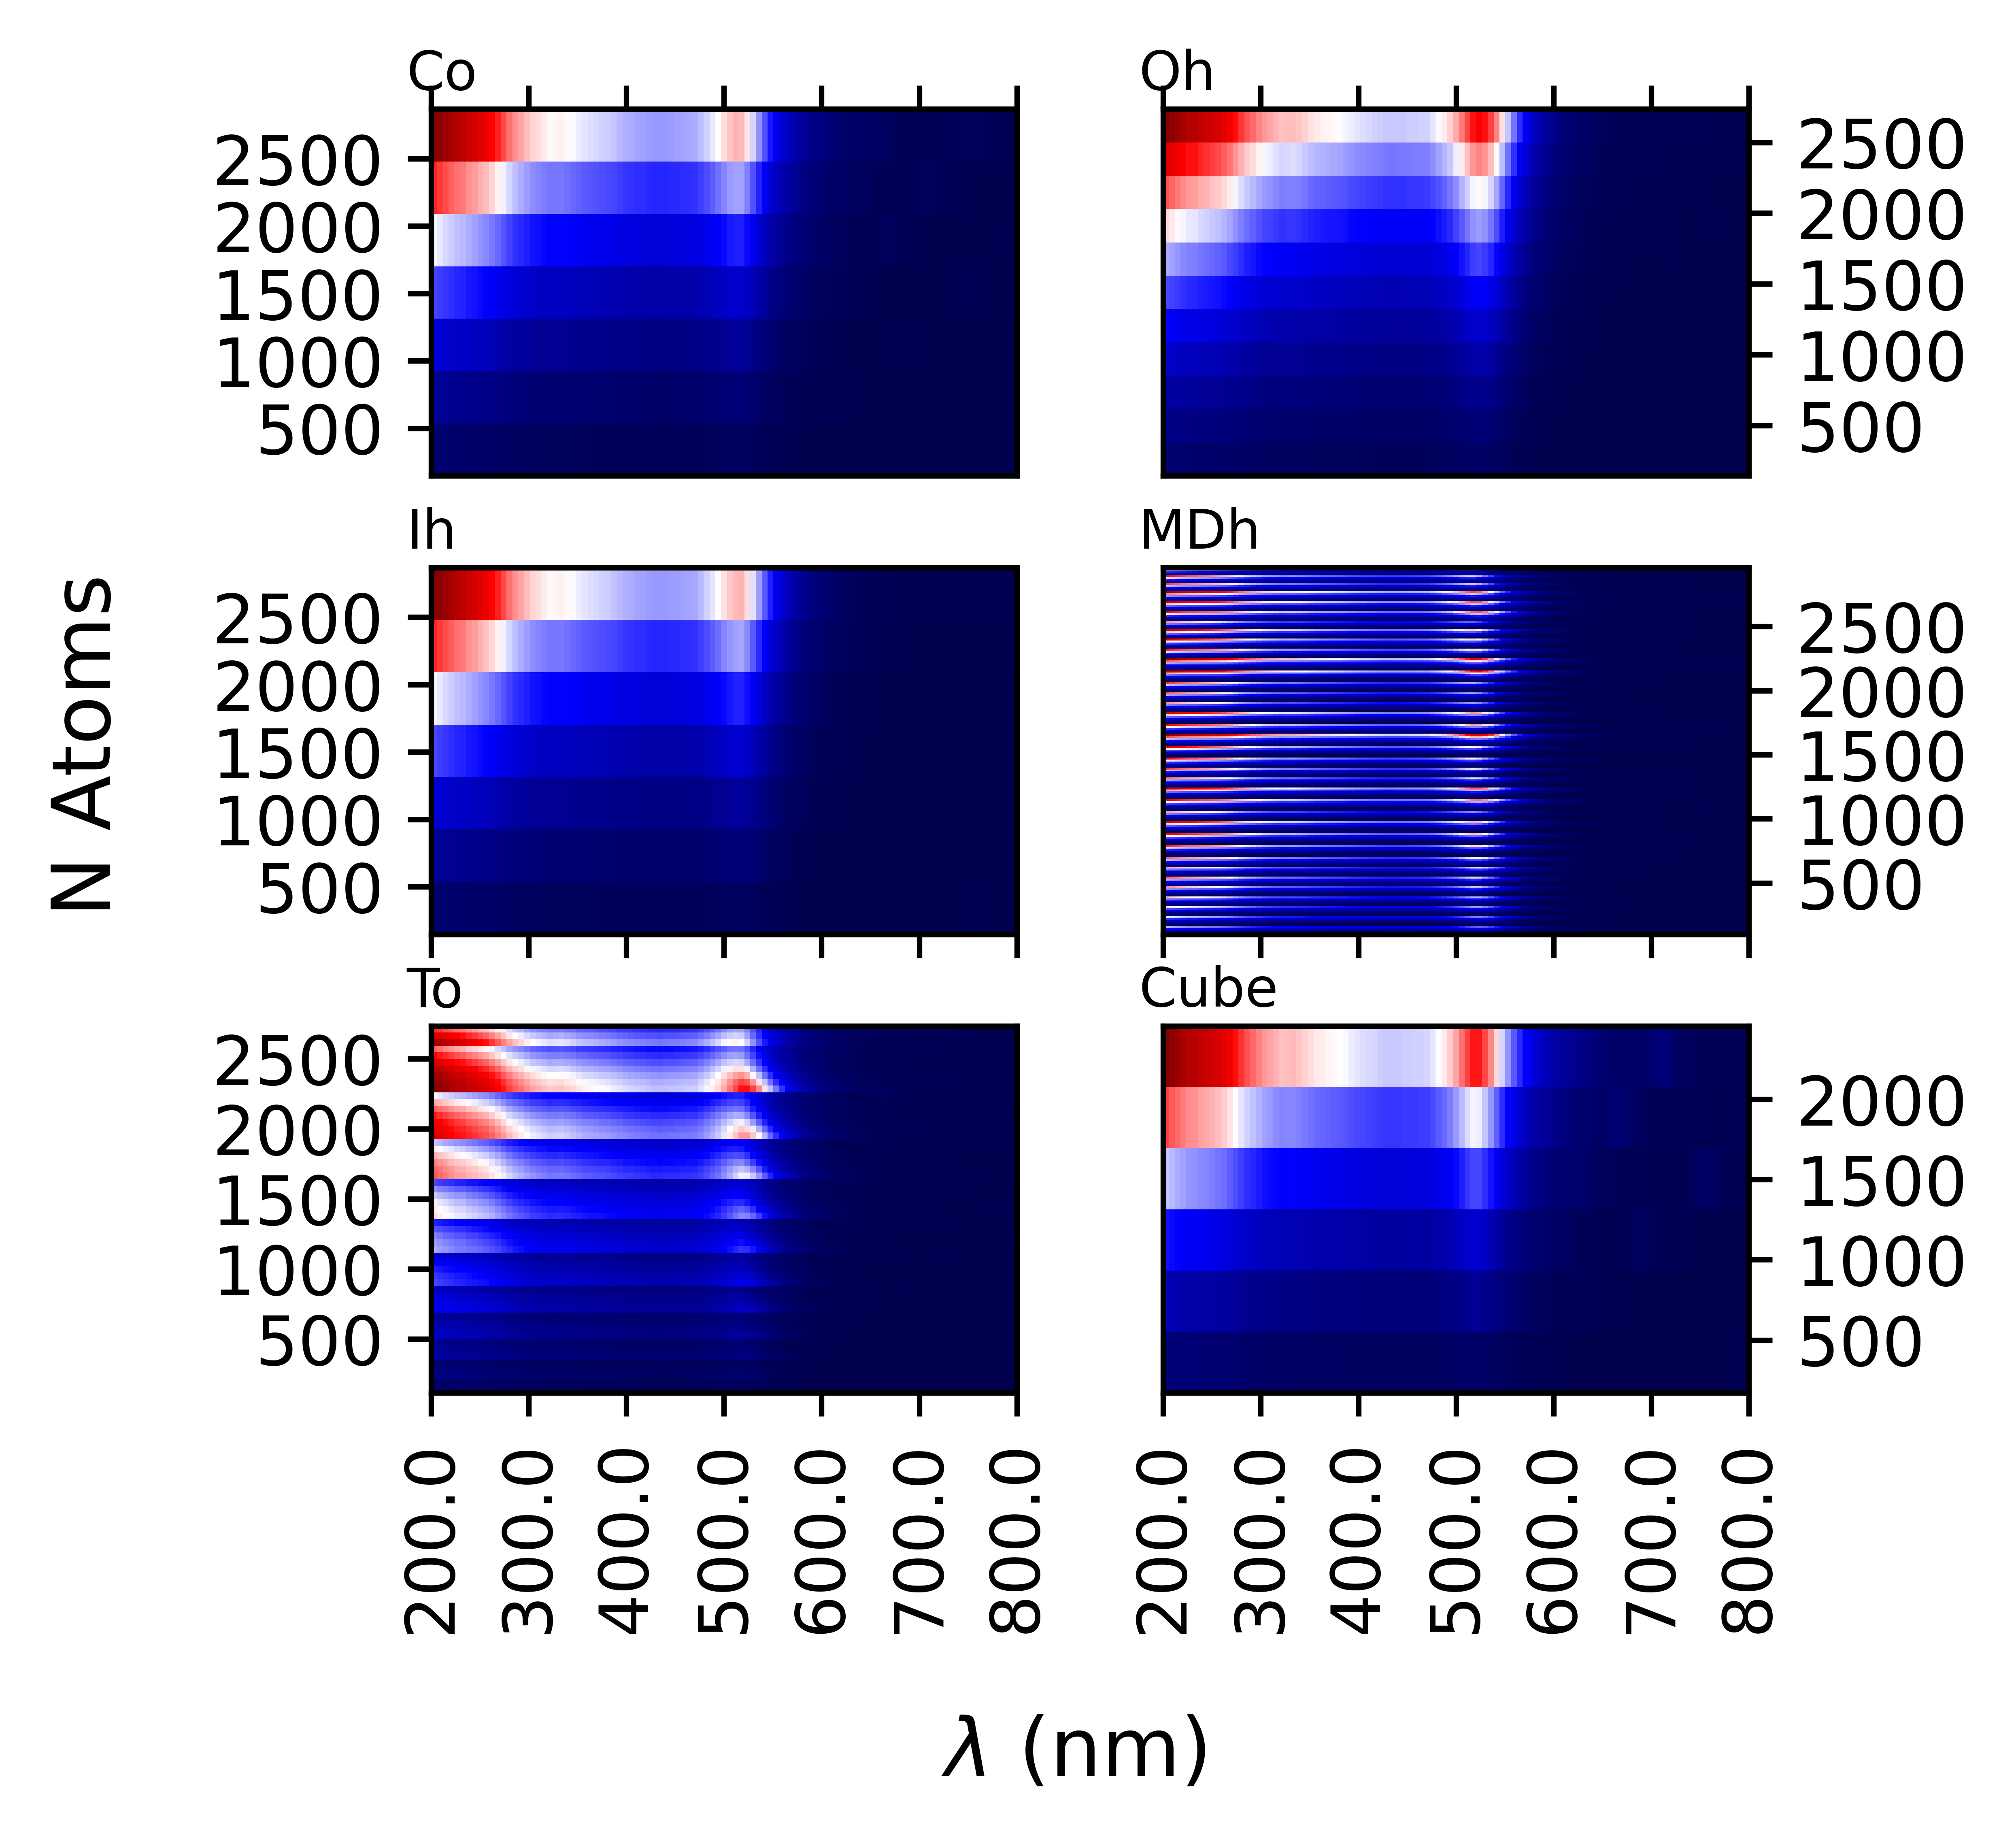
\includegraphics[width=0.95\textwidth]{figures/LM/GDM/Au_Specs.png}
    \caption{Extinction spectra of varied size and morphology for Au clusters. Structures considered are a subset of those introduced in Figure \ref{Fig:nanoparticles_sizes}.}
    \label{Fig:Size_Au_GDM}
\end{figure}

\begin{figure}[b]
    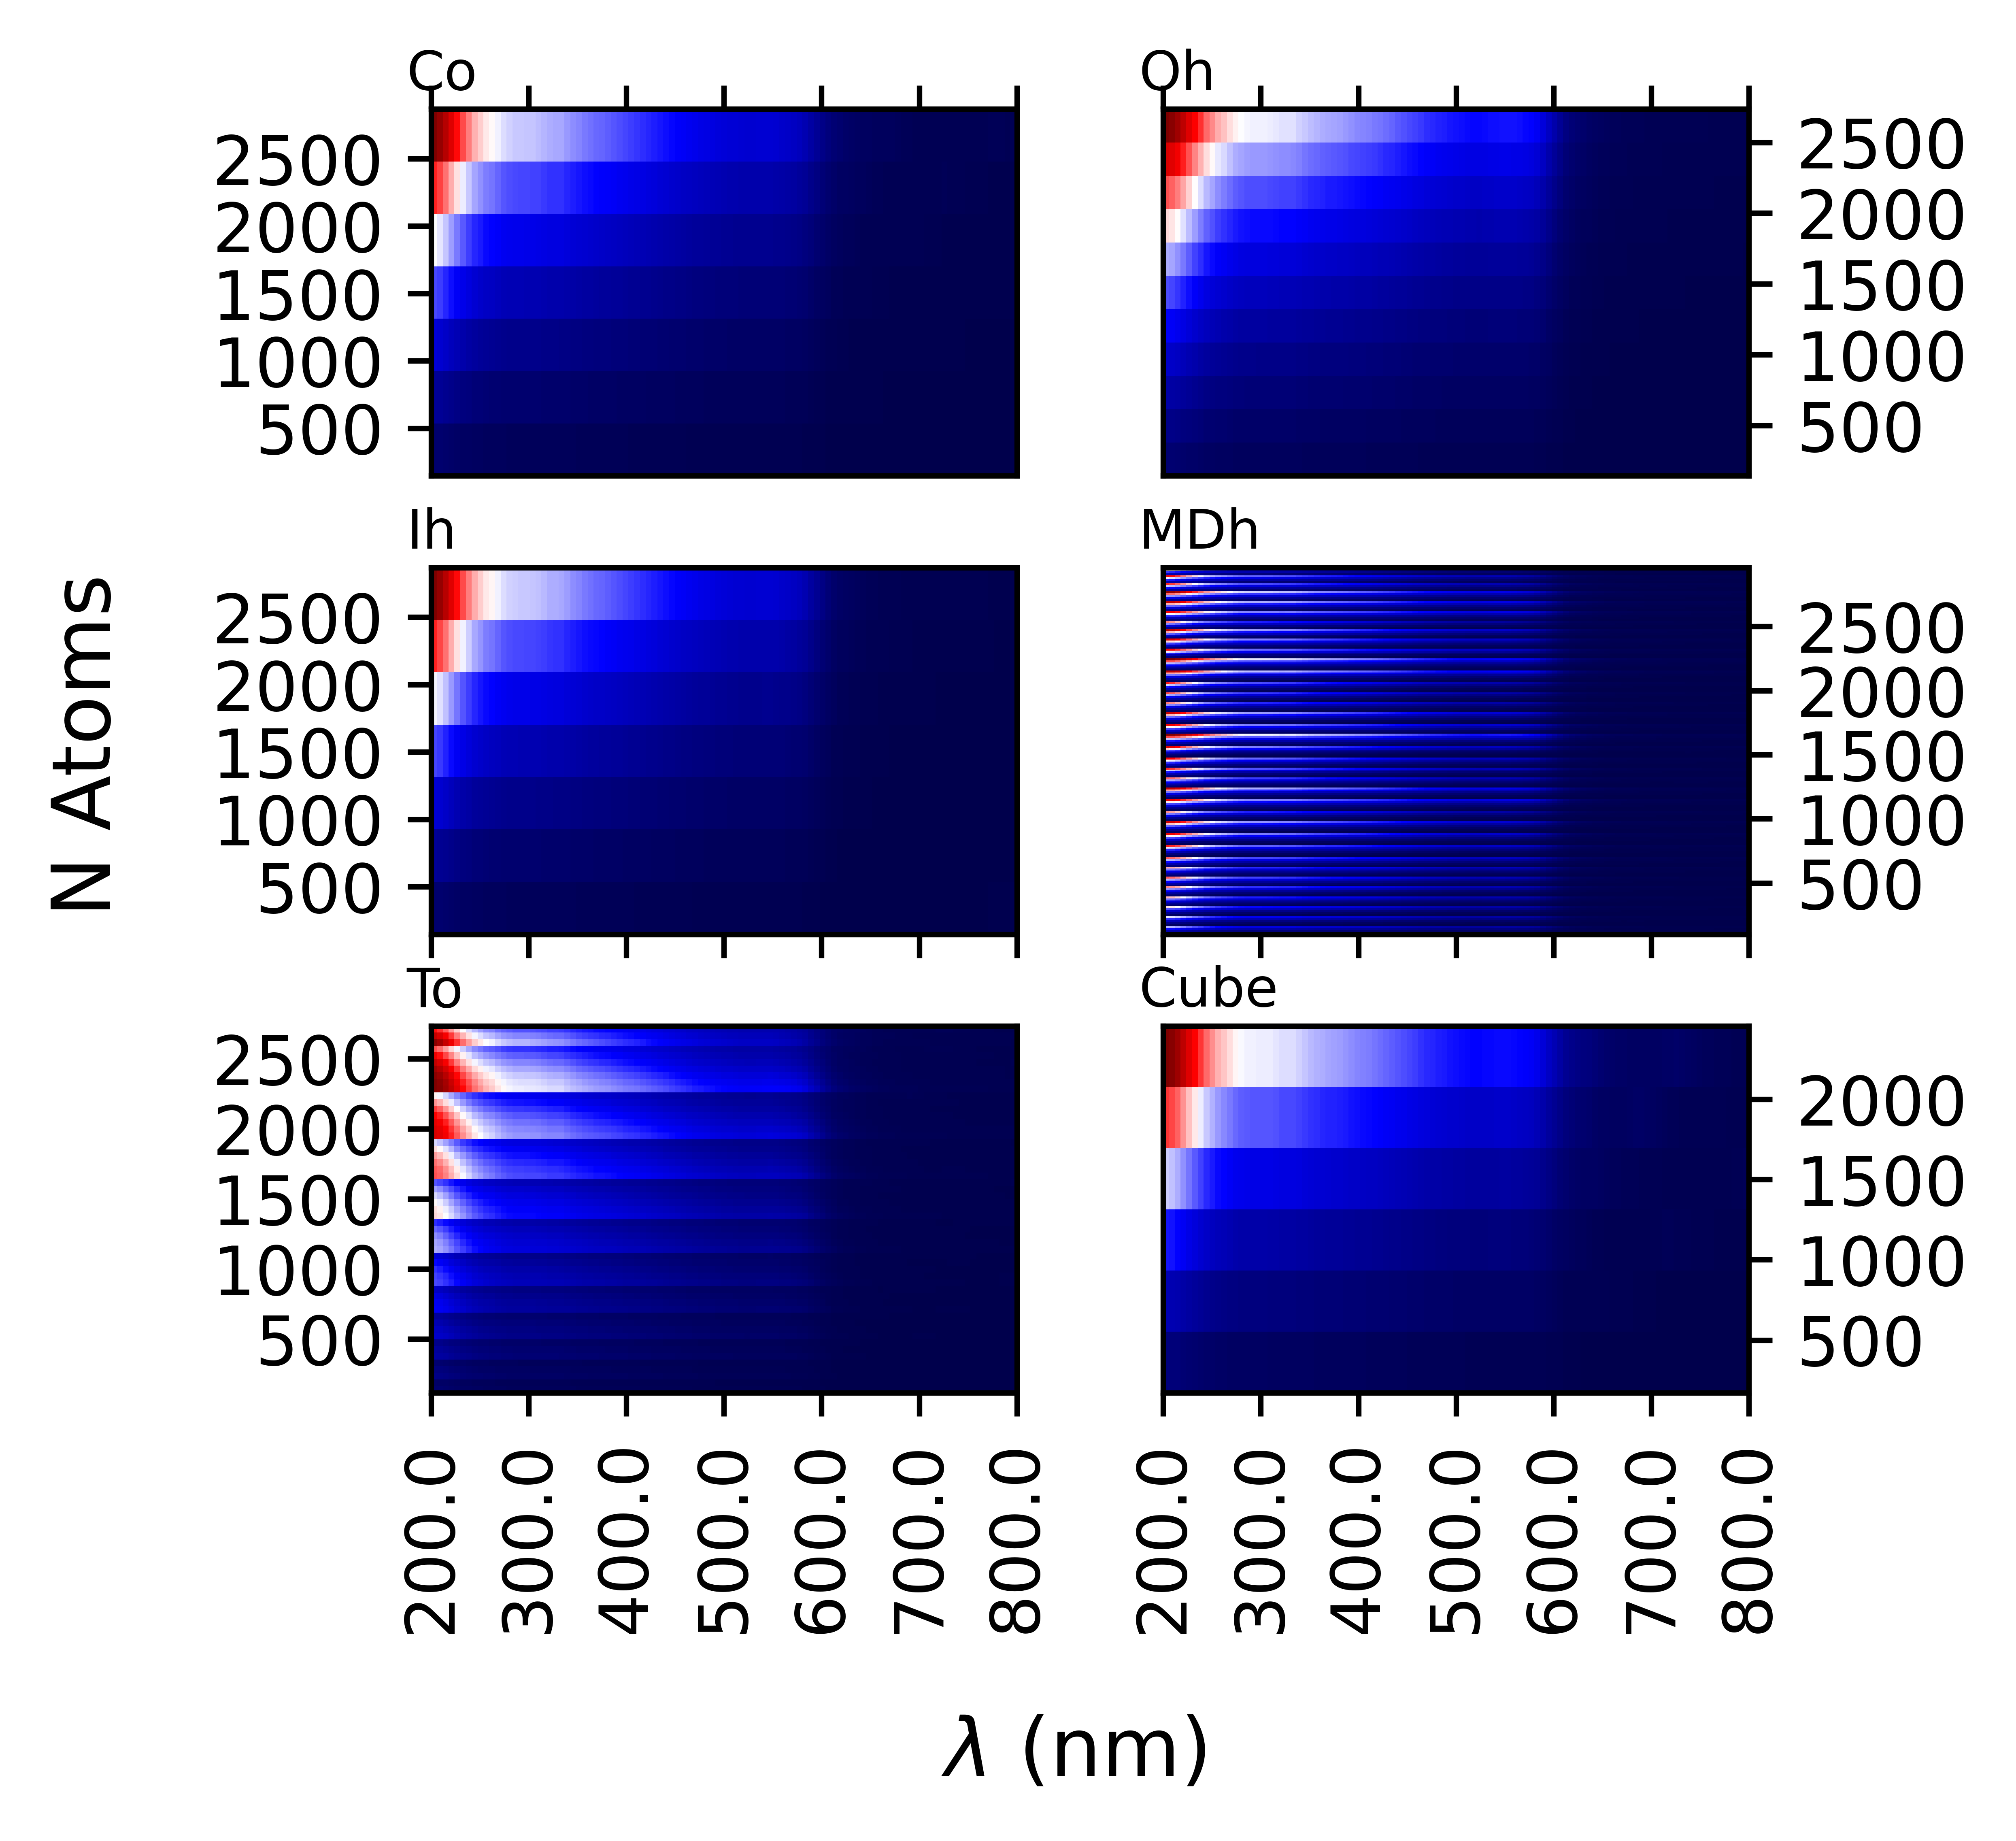
\includegraphics[width=0.95\textwidth]{figures/LM/GDM/Cu_Specs.png}
    \caption{Extinction spectra of varied size and morphology for Cu clusters. Structures considered are a subset of those introduced in Figure \ref{Fig:nanoparticles_sizes}.} 
    \label{Fig:Size_Cu_GDM}
\end{figure}

\begin{figure}[b]
    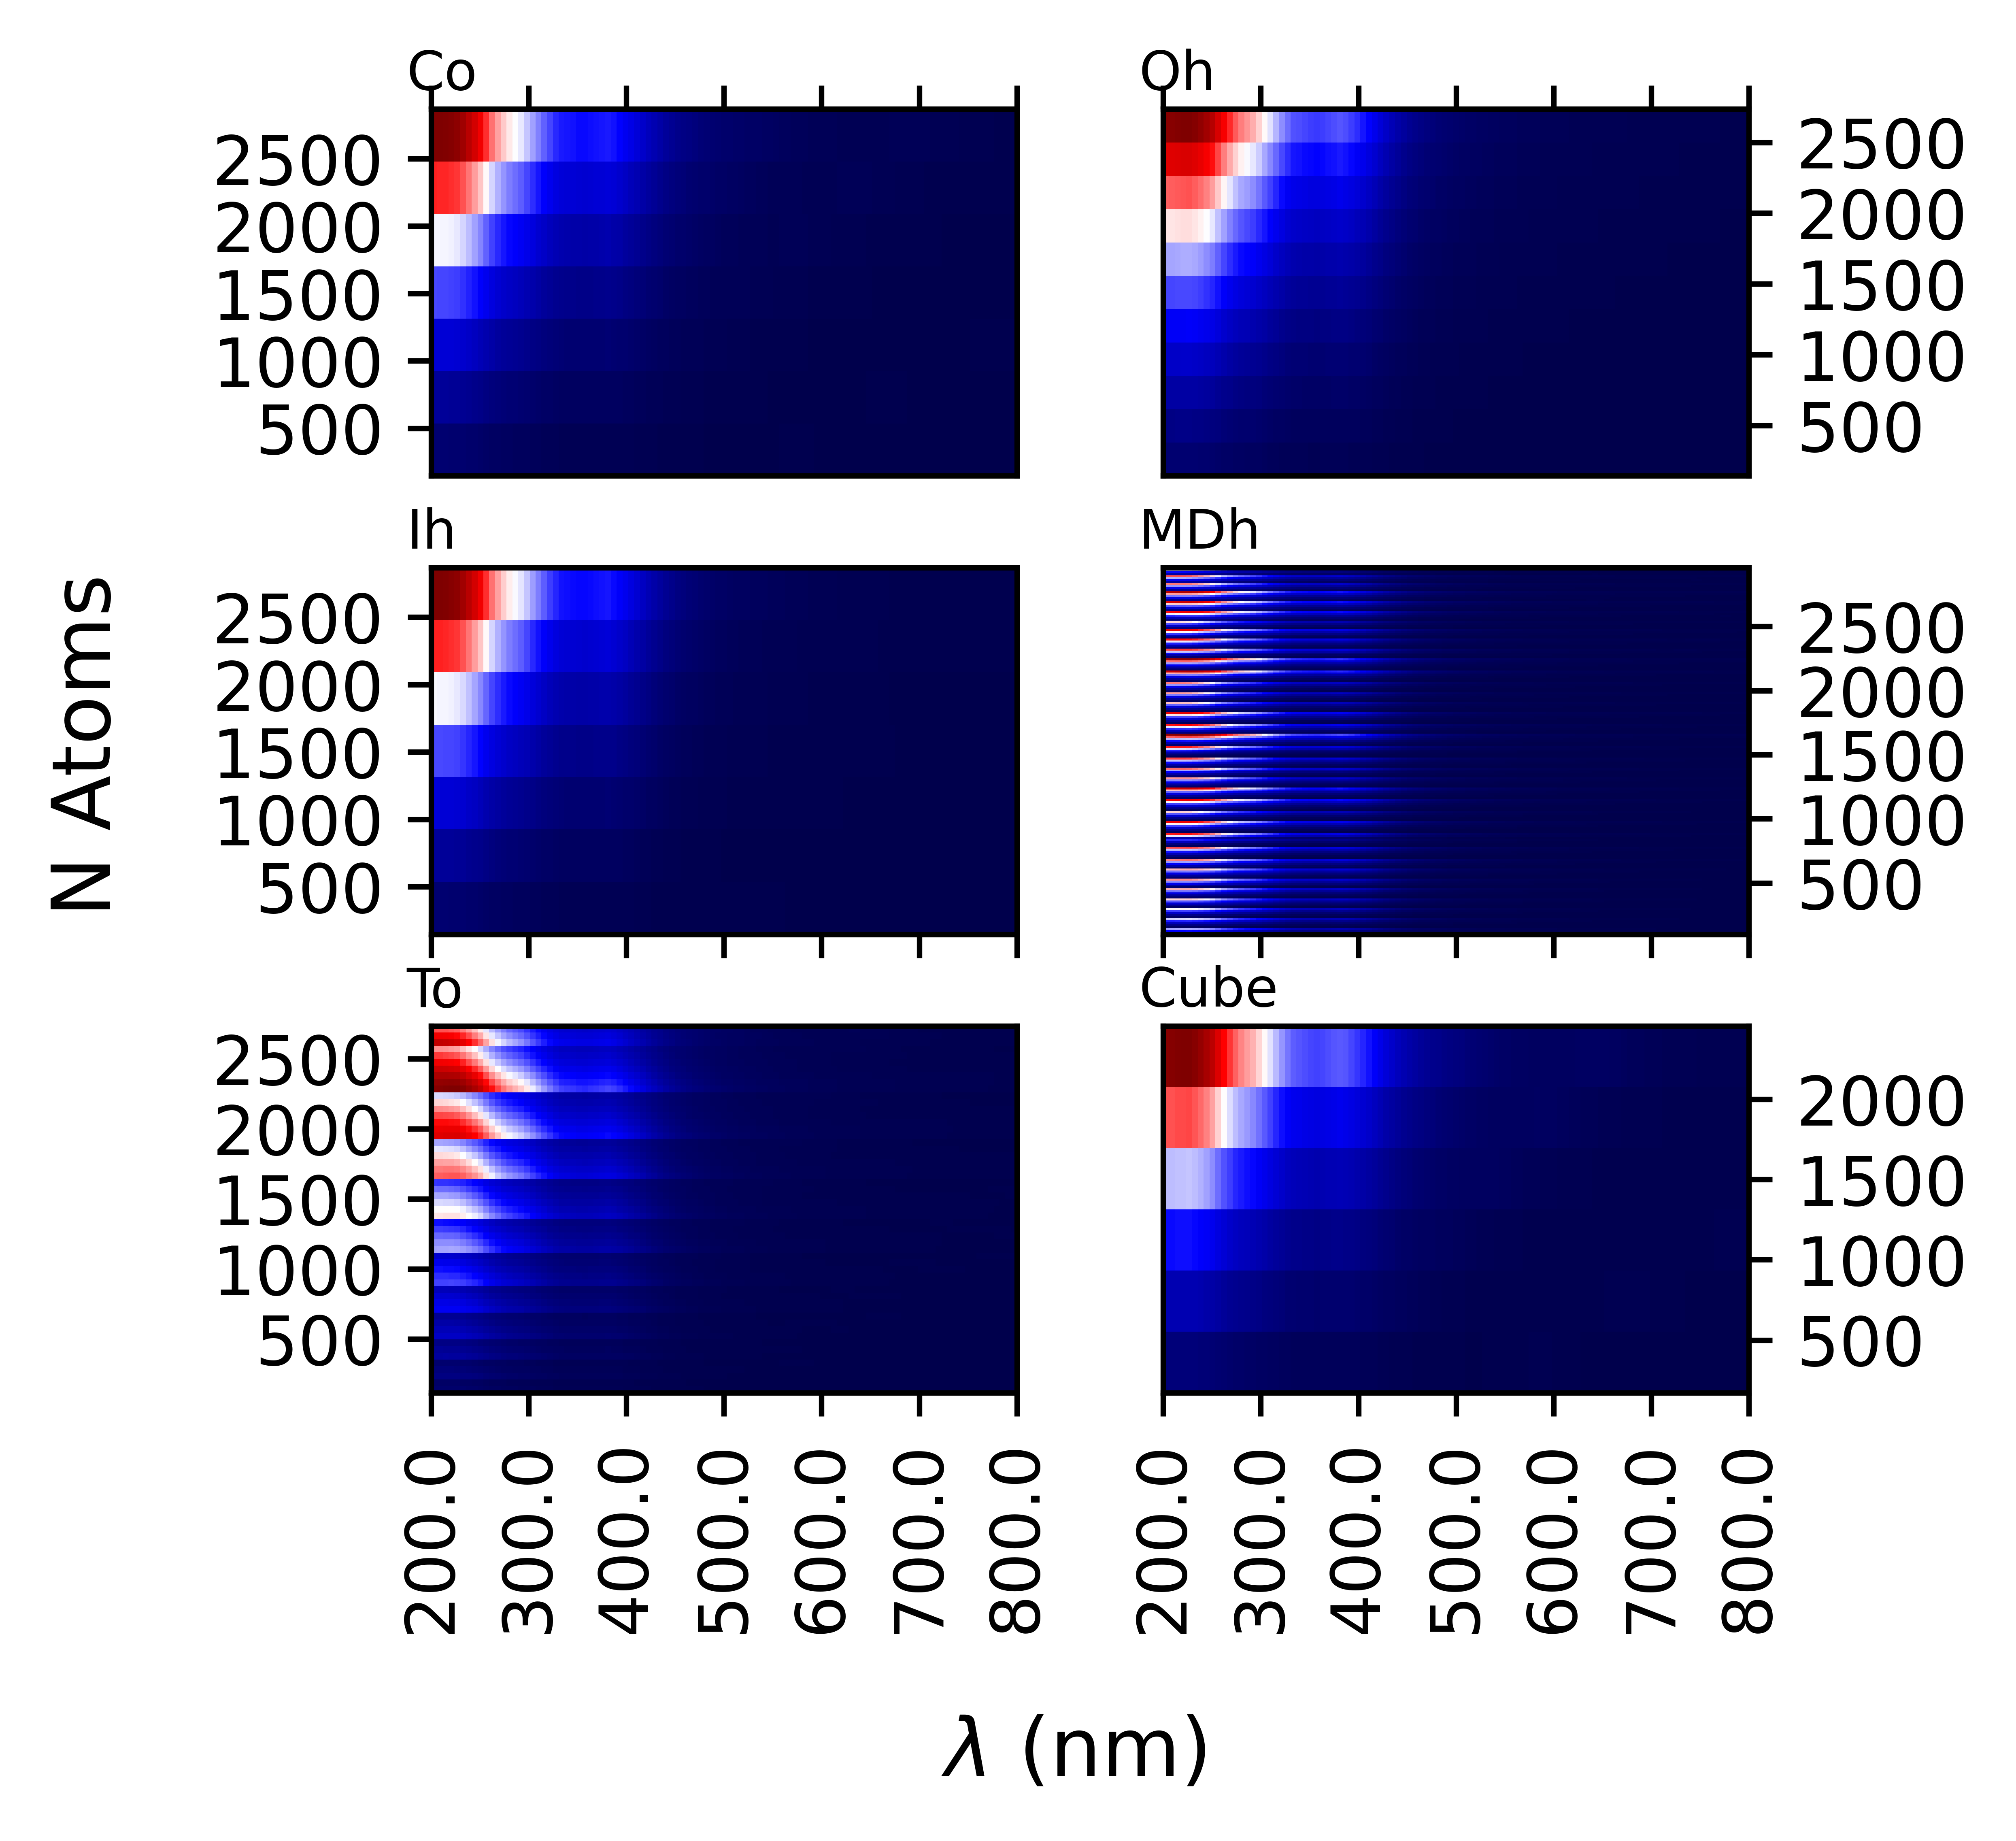
\includegraphics[width=0.95\textwidth]{figures/LM/GDM/Pt_Specs.png}
    \caption{Extinction spectra of varied size and morphology for Pt clusters. Structures considered are a subset of those introduced in Figure \ref{Fig:nanoparticles_sizes}.}
    \label{Fig:Size_Pt_GDM}
\end{figure}

In consideration of Figure \ref{Fig:Size_Ag_GDM}, Figure \ref{Fig:Size_Au_GDM}, Figure \ref{Fig:Size_Cu_GDM}, Figure \ref{Fig:Size_Pt_GDM}, it is already clear that the model is sensitive to both the size of nanocluster; manifested primarily as the intensity which scales linearly with the number of atoms; and the morphology. This first statement should not be surprising, as by increasing the number of interacting dipoles, so too do we increase the aggregate effect of these dipoles in absorbing or scattering incoming light. However, the fact that the model is sensitive to the morphology of the given cluster is fascinating when considering that the model only truly cares about the interaction of a dipole with respect to other dipoles and the incident field.

However, this sensitivity motivates our continued use of the approach as an interim model between a fully atomistic \textit{ab initio} technique such as TDDFT, and a complete finite element method in which one has a less precise control over the features and structures considered. Of worthy note is the MDh plot for Ag in Figure \ref{Fig:Size_Ag_GDM} wherein we observe striations in the extinction spectrum which appear to line up with the striations in the number of atoms vs surface area plot of \ref{Fig:NPs_MDh}. We see the precise same phenomenon for the To morphology in \ref{Fig:Nps_To} for the Ag extinction spectrum. Whilst these features likely exist for the other metals, too, the effect may be difficult to detect for less optically active species since Ag is known for being particularly resplendent with respect to its optical features in the UV-Vis range.

Nonetheless, given that the model is sufficiently descriptive of the modelled metals by construction, and it satisfies the need for it to be size and morphology sensitive, then we are confident in continuing to use it to describe mesoscale systems which are beyond the reach of \textit{ab initio} methods. For a comparison between spectra recovered from the GDM model and TDDFT methods, we refer the reader to our work in Reference \cite{Wei} in which we identified a general lack of agreement between the two methods at a size scale where TDDFT~-~based approaches are appropriate. As discussed in the previous section, this disagreement may indeed arise from not having considered necessary, explicit, quantum mechanical interactions within the nanoparticles. We may close by reflecting that when traversing the multi~-~scale modelling ladder, it is not common for methods at different levels of theory to return near identical results.

\clearpage
\section{The effect of Pt doping}
\label{sec:AuPt_DFT}

We describe the computational methods employed, motivating their use given the context. In doing so, we demonstrate rich electrostatic, and electrodynamic properties of the Au nanoparticles. We proceed to elucidate upon the aforementioned computed quantities, drawing conclusions from our results given the computed behaviour and physics known \textit{a priori}. Finally, we present and justify our primary conclusion - that the complex interplay occurring at the nanoscale has profound consequences on the opto-electronic features of NAs which we strongly suspect is significant when considering their efficacy as a plasmocatalyst. We show that the HOMO - LUMO gap of two Au$_{20}$ isomers can be finely tuned by displacing the Pt impurities as either a substitution or an adatom. By calculating the absorption spectra, in conjunction with the projected density of states (PDoS), we show clearly the importance of knowing the precise geometry when considering such complex NAs.

We present the findings of this project as follows. A detailed analysis of the ground-state properties, and of the optical spectra with respect to the changes in geometry and chemical ordering. Finally, we provide at the end of the section a discussion on the observed changes of the HOMO - LUMO gap, the PDoS, and the computed spectra at both the classical and quantum mechanical level of theory.

Our two initial structures of Au$_{20}$ were a C1 point group symmetry (left column of Figure \ref{Fig:Sites}) and the well-studied tetrahedron (Th) (right column of Figure \ref{Fig:Sites}). The former low-symmetry structure was obtained via a single-atom deposition upon the double-icosahedron with 19 atoms at room temperature and then ionic relaxation at density functional level. After ionic relaxation, we have not recognised any significant structural changes suggesting the shape is a local minimum. The rationale behind this selection is twofold. First, limiting our analysis to the theoretical general minimum, $Au^{Th}_{20}$, provides a simple scenario that can be difficult to generalise. Second, we opt for a low symmetry motif as pump/probe experiments have shown local heating effects associated with the high-intensity laser. Hence, there is a not negligible probability that Au$_{20}$ will not be in its global minimum but resides in a low-symmetry local minimum.

The latter high-symmetry structure is the energetically more favourable at this size, as confirmed by our calculations in agreement with the literature \cite{Rapacioli2018,Gruene2008}. Our intention here being to simultaneously probe the effects of alloying on small Au clusters, and the effects that the seed morphology itself may have. For each system, we replace Au atoms from the initial structure with Pt, such that particle number is conserved. We have also adopted the approach of introducing the Pt defect as an ad-atom so as to better replicate, at a smaller scale, the design described in the work of Salmon \textit{et al.} \cite{JorgeStructure}. 
Whilst it is true that a vast array of both high and low symmetry structures exist at the size scale considered, we have performed this particular investigation on these two in particular such that they may serve as examples of such morphological variation at this scale. That is to say that this work may serve as a case-study from which further investigations into the structure - properties relationship may be performed.

\begin{figure}
\centering
\begin{subfigure}[b]{0.45\textwidth}
    \centering
    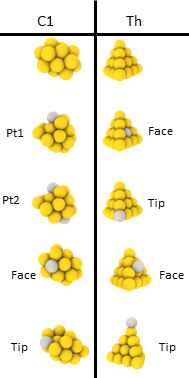
\includegraphics{figures/LM/AuPt_EPJ/Structures.png}
    \caption{Au$_{20}$ isomers (row 1) considered for study.}
    \label{Fig:Sites}
\end{subfigure}
\begin{subfigure}[b]{0.45\textwidth}
    \centering
    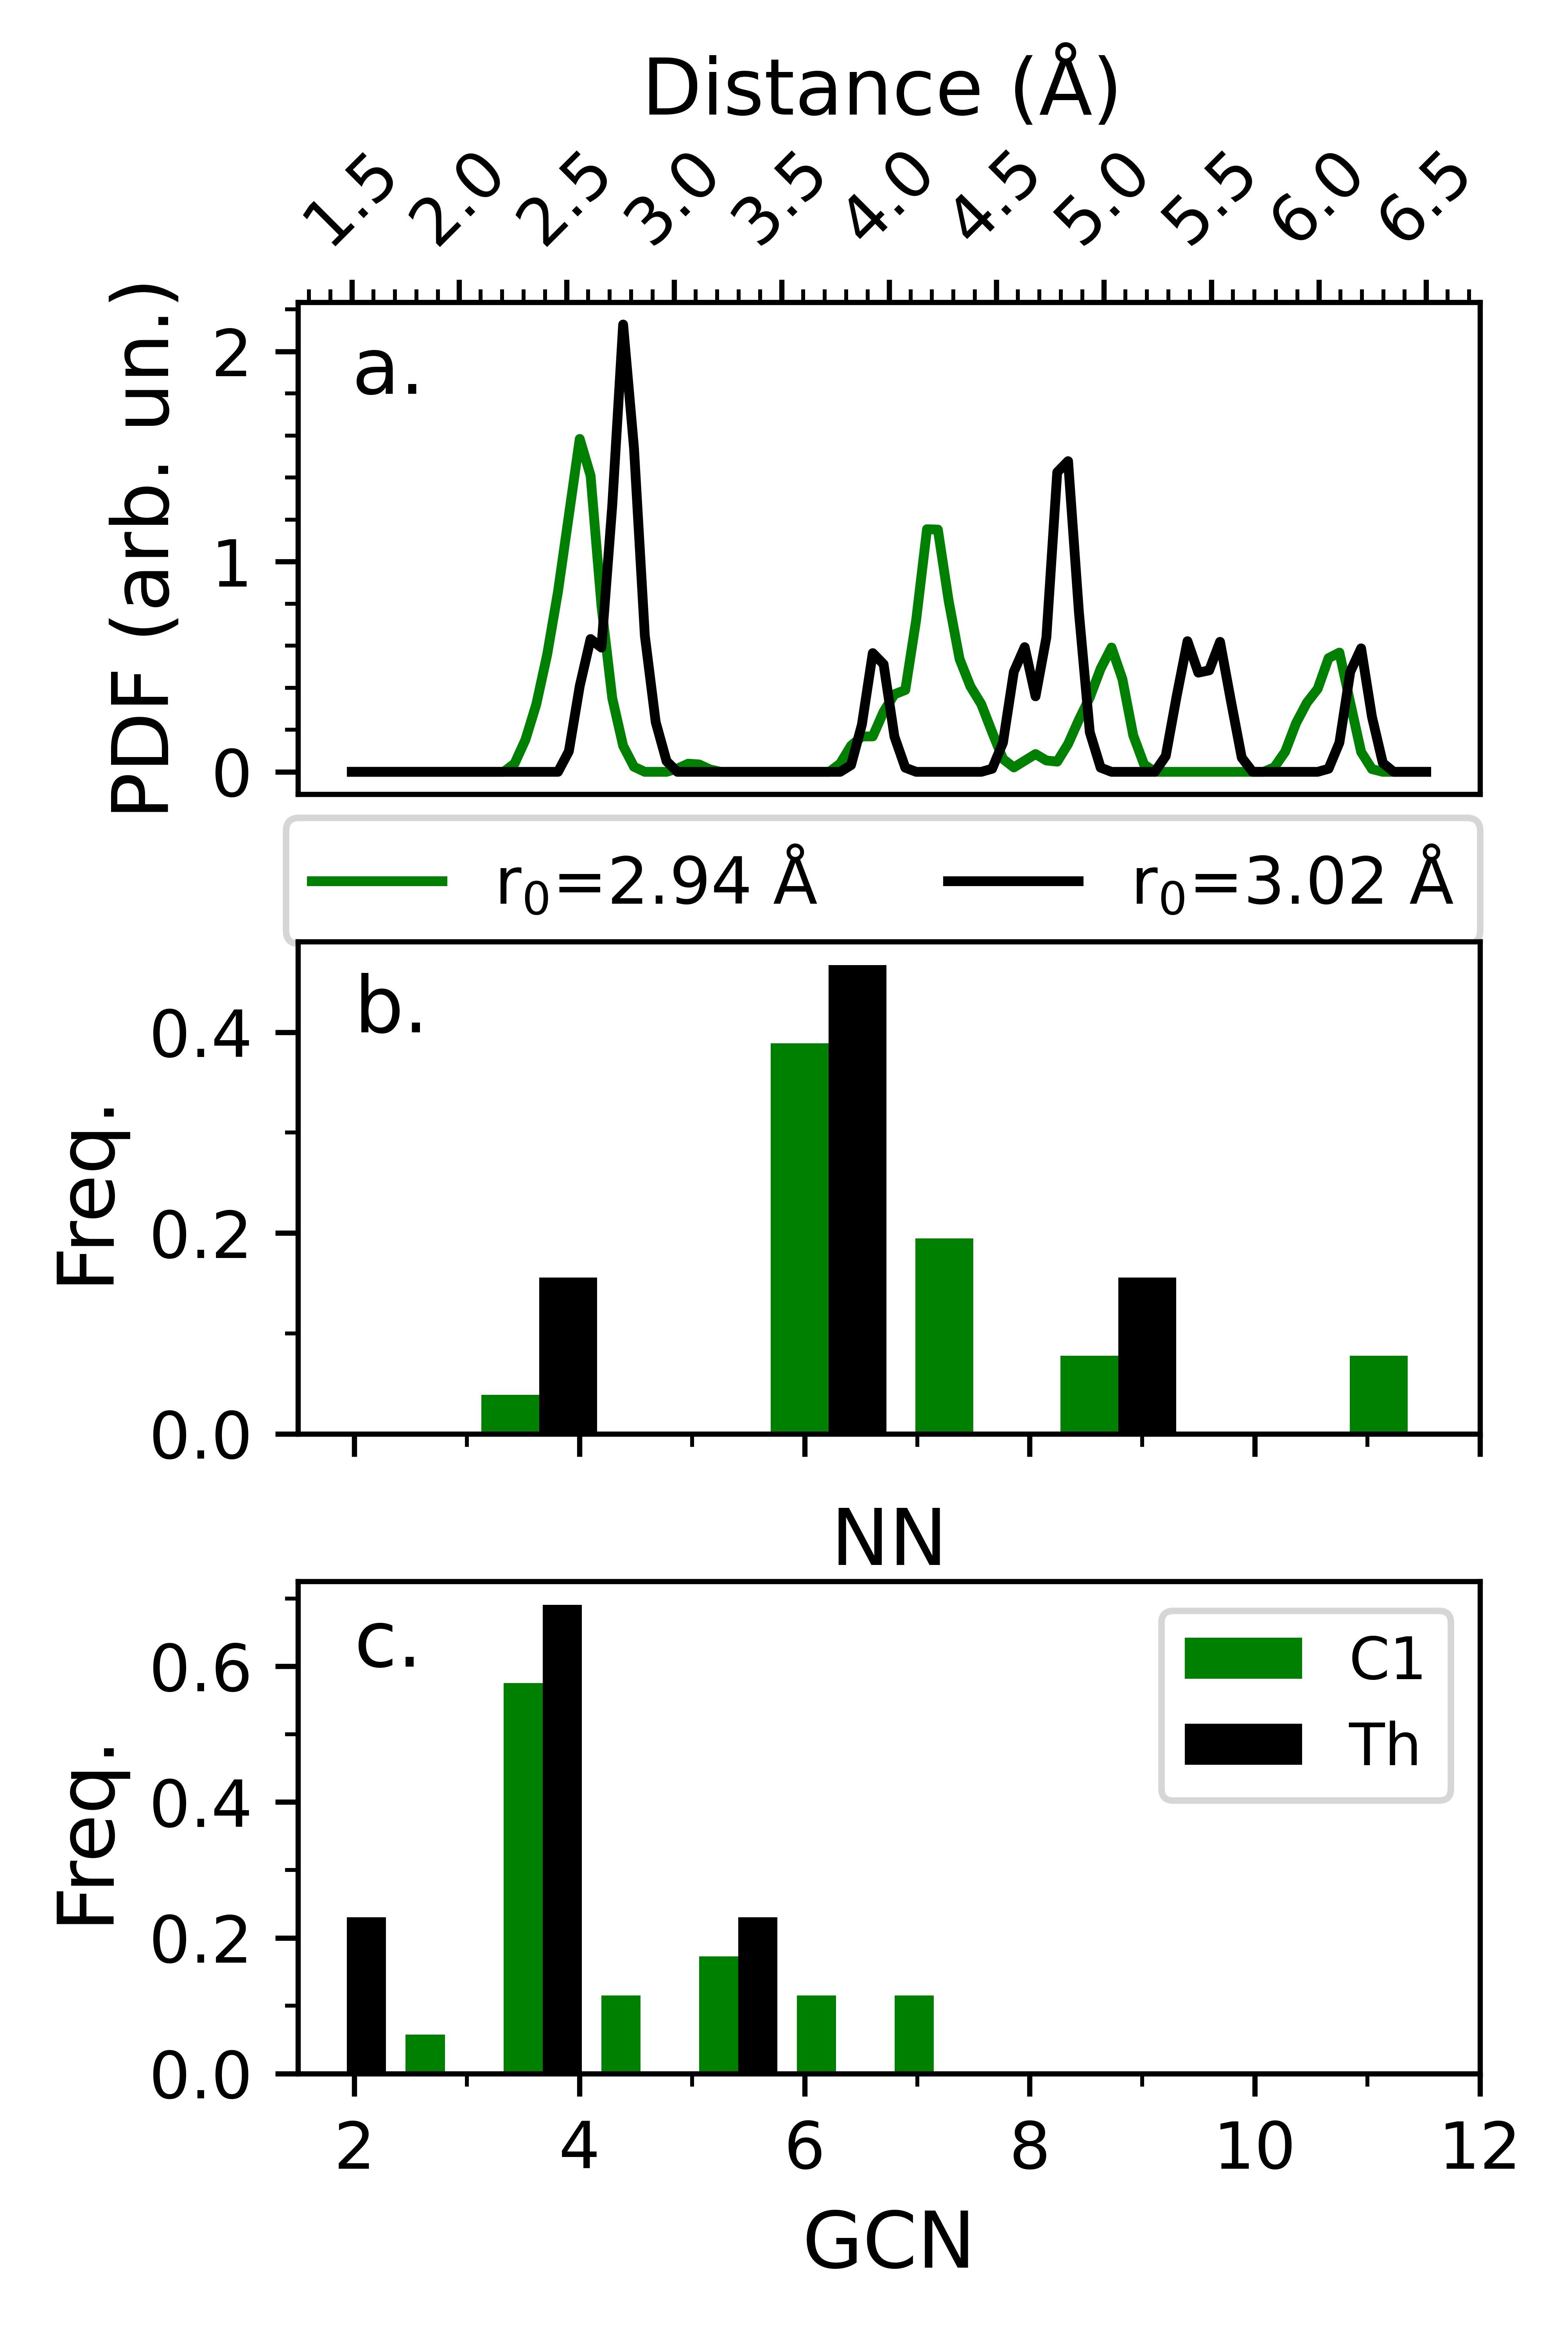
\includegraphics{figures/LM/AuPt_EPJ/Th_C1_Comp.jpeg}
    \caption{Structural descriptors of pure Au NPs.}
    \label{Fig:Compare}
\end{subfigure}
\caption{Structural information comparing the nanoalloys considered in this study. (\textbf{a}) Top row - pure Au. Rows 2 and 3 - doped structures. Rows 4 and 5 - Ad-Atom. (\textbf{b}) Top panel, a. the PDF. Central panel, b. the distribution of atomic coordination numbers. Bottom panel, c. the distribution of CN. The insert in the top panel reports the average first neighbour bond length, calculated as the first minimum of the PDF.}
\label{Fig:Au20_Struts}
\end{figure}


We present in Figure \ref{Fig:Compare} structural discrepancies between the well-known Th structure, and the novel C1 isomer. We report the pair distance distribution function (PDF) (Figure \ref{Fig:Compare}a) which details the relative distance between pairs of atoms within the cluster. We may use this as a measure of the level of amorphicity by considering the broadness and spread of the peaks. Moreover, we use this to approximate the average first neighbour distance, $r_{0}$, by finding the location of the first minimum. We define $\Omega_i$, the neighbourhood around atom $i$, as the set of atoms whose distance from the atom $i$ is smaller than $r_0$. We have also presented two distributions describing the atomic coordination numbers (Figure \ref{Fig:Compare}b and c). Each details the type of local atomic environment which may be found within the nanoparticle. We shall use these quantities to better elucidate on the structural properties of the NAs by computing the coordination number, $NN$; and the generalised coordination number (GCN) \cite{ActivityGCN}, Figure \ref{Fig:Compare} shows three LAE with a view to better appreciate the variations in NA morphology when developing the structure - properties relationship throughout the text. We motivate the introduction of this quantity to better distinguish between C1 and Th as this measure provides a more variegated description of the local atomic environment. Later on, we shall also utilise the average coordination number of the introduced Pt, $\overline{NN_{Pt}}$.

We note the broader PDF curves on the upper panel for the C1 Au nanoparticle (green curve) compared with the much finer PDF curve of the Th Au nanoparticle (black curve). We observe the reduction in the average first neighbour bond length in addition to profound changes in the distribution of the atomic coordination number. The latter of which demonstrates how much more compact the C1 cluster is relative to the Th. Finally, we demonstrate the utility of the CN when considering NAs - in that one may observe the finer detail of atomic distributions otherwise inaccessible by considering the coordination number only.

In the instance of the introduction of a Pt dopant via direct substitution, we selected the high symmetry site of tips, and lower symmetry sites of facets to introduce the defect as seen in Figure \ref{Fig:Sites}. For introducing ad-atoms, we adsorbed Pt into hollow, and atop configurations. For each structure, we perform a classical geometry optimisation with the FIRE \cite{Fire} algorithm as implemented in the atomic simulation environment (ase) and asap3 python packages \cite{ase-paper,asap3}, using inter-atomic potentials of the RGL form \cite{RGL} with parameters provided by Baletto \textit{et al}. \cite{RGL_Pot}. We motivate the choice of classical potentials in the near equivalence of the relaxed structures when computed via \textit{ab initio} or classical methods. Hence, in the interest of minimising computational overheads, we elected to relax all structures with the FIRE algorithm. We note that the inclusion of Pt into the C1 structure led to noticeable structural rearrangement, particularly in the instance of doping.

From a classically optimised structure, we proceed to compute the ground state electronic density - recording its density of states (DoS), its atomic projected density of states (PDoS), and the HOMO - LUMO gap, $\varepsilon_{G}$. From a sufficiently well-converged ground state, we proceed to evolve each system in time by approximating the enforced time-reversal symmetry (AETRS) \cite{aetrs} to evaluate the time evolution operator. A time step of 0.33 attoseconds is used, and all systems are evolved for 16.5 fs.

We compute the ground state properties of the considered structures in Figure \ref{Fig:Sites}. We monitor the changes to $\varepsilon_{G}$ in Table \ref{tab:table} as the Au$_{20}^{Th}$ is known to have a $\varepsilon_{G}$ to be approximately 1.7~eV \cite{Au20Homo_Lumo,Baletto2015}. We have determined this gap, with our 5d$^{10}$6s$^{1}$ electronic configuration pseudopotential and within the LDA, to be 1.52~eV which is sufficiently representative of the physics of this cluster. Table \ref{tab:table} reports how altering the morphology and Pt loading of the cluster affects this fundamental feature of the NA. As found for other doping \cite{Baletto2015}, the presence of Pt can both reduce or enlarge $\varepsilon_{G}$. 
We observe that, with the exception of the slight increase in HOMO- LUMO gap of Th-Dope-Tip by 30 meV, a more symmetric ionic structure may lead to a larger $\varepsilon_{G}$. As such, we find that by introducing Pt into low symmetry environments, we may reduce the size of the gap.
%
\begin{table}[ht!]
\centering
\caption{Effects of Pt doping of two isomers of Au$_{20}$ on the HOMO - LUMO gap, average first neighbour bond length, average total NN, average Pt NN, average Pt GCN where appropriate, and symmetry information. All structures are ordered as they appear in Figure \ref{Fig:Sites}.}
\label{tab:table}
\begin{tabular}{lllllllll}
\hline\noalign{\smallskip}
 & Structure & $\varepsilon_{G}$ [eV] & r$_{0}$ [\AA]& $\overline{NN}$ & $\overline{NN_{Pt}}$ & $\overline{GCN_{Pt}}$ & Schoenflies &  Order  \\
\noalign{\smallskip}\hline\noalign{\smallskip}
\multicolumn{1}{l|}{\multirow{5}{*}{C1}} & \multicolumn{1}{l|}{Pure} & 0.03 & 2.94 & 7.2 & N/A & N/A  & C$_{1}$ & 1      \\
\multicolumn{1}{l|}{}                    & \multicolumn{1}{l|}{Dope-Pt$_1$} & 0.12 & 3.12 & 6.4 & 4.0 & 2.17 & C$_{1}$ & 1    \\
\multicolumn{1}{l|}{}                    & \multicolumn{1}{l|}{Dope-Pt$_2$} & 0.58 & 3.07 & 6.4 & 5.0 & 2.92 & C$_{1}$ & 1    \\
\multicolumn{1}{l|}{}                    & \multicolumn{1}{l|}{Adatom-Face} & 0.08 & 3.17 & 6.6 & 6.0 & 3.50 & C$_{1}$ & 1    \\
\multicolumn{1}{l|}{}                    & \multicolumn{1}{l|}{Adatom-Tip}  & 0.24 & 3.07 & 6.3 & 4.0 & 2.17 & C$_{1}$ & 1    \\
\noalign{\smallskip}\hline\noalign{\smallskip}
\multicolumn{1}{l|}{\multirow{6}{*}{Th}} & \multicolumn{1}{l|}{Pure} & 1.52 &  3.02 & 6.0 & N/A & N/A  & T$_{d}$ & 24    \\
\multicolumn{1}{l|}{}                    & \multicolumn{1}{l|}{Dope-Face} & 1.24 & 3.02 & 6.0 & 9.0 & 5.25 & C$_{3}$ & 3     \\
\multicolumn{1}{l|}{} &
\multicolumn{1}{l|}{{Dope-Tip}} & 1.55 & 3.02 &  6.0 & 3.0 & 1.50 & C$_{3}$ & 3  \\
\multicolumn{1}{l|}{}                    & \multicolumn{1}{l|}{Adatom-Face}  & 0.55 & 3.02 & 6.0 & 3.0 &  2.00 & C$_{1}$ & 1\\
\multicolumn{1}{l|}{} &
\multicolumn{1}{l|}{Adatom-Tip}  & 0.33 &  3.02 & 5.81 & 1.0 & 0.33 & C$_{3}$ & 3 \\

\end{tabular}
\end{table}

In considering Table \ref{tab:table}, we note that there does not appear to be a general trend emerging between $\varepsilon_G$ and the location, or indeed quantity, of the Pt. However, a curious property emerges for the Au$^{Th}_{20}$ as an independent isomer. That being that the way in which we introduce Pt will influence strongly the closing of the gap. By adsorbing Pt onto the perfect structure, we are able to shrink the gap to up a factor of five. Conversely, if we simply perform the substitution, we observe no such influence on the gap.

Alternatively, by considering the Au$^{C1}_{20}$ structure, we actually observe the opposite behaviour. By introducing Pt to a low symmetry structure, we are able to open up a near non-existent gap. Indeed, when considering the lower left structures of Figure \ref{Fig:Sites}, we see that geometrically relaxed structures arising from this isomer assume a vastly different conformation depending on the location and quantity of introduced Pt. Already, this disparity is in itself worthy of comment. A highly symmetric Au isomer remains structurally unperturbed, regardless of the method of Pt injection, whereas a low symmetry isomer is  prone to disruption in the presence of a Pt dopant.

Moreover, by considering the geometrical properties presented in Table \ref{tab:table}, we observe a considerable difference between how the Th and C1 accept a Pt atom. In the instance of the former, we see no appreciable change to the geometry as a consequence of introducing Pt either through doping or adsorption. Conversely, C1 demonstrates profound instability relative to its initial, unperturbed configuration. This is mostly evident in the rapid differences in the average first neighbour bond length, and the average atomic coordination number of the cluster.

In Figure \ref{Fig:C1Dos} and Figure \ref{Fig:ThDos}, we demonstrate the orbital characteristic, via the calculation of the atomic PDoS, of the electronic states up to the HOMO and for the following 10 unoccupied orbitals. As discussed earlier in the chapter, the fashion by which the PDoS is computed aims to preserve the character of the pseudo-atomic orbital which results in the two quantities not necessarily integrating to the same value. Hence the slight discrepancies observed in Figure \ref{Fig:C1Dos} and Figure \ref{Fig:ThDos} between the reported DoS and PDoS. To create the figures, we have performed a Lorentzian broadening with a width of 217 meV around each of the Kohn-Sham eigenstates to smooth out the DoS, and to make interpretation of detail more facile. We are able to finely probe the nature of the HOMO - LUMO gap, as reported in Table \ref{tab:table}, by considering nature of the atomic orbitals in the vicinity of these states. One might note that the LUMO has often a strong $p$-character. The nature of the HOMO orbital is more system-dependent but in several cases the HOMO is a combination of $pd$-type orbitals. 


\begin{figure}
\centering
\begin{subfigure}[b]{0.45\textwidth}
    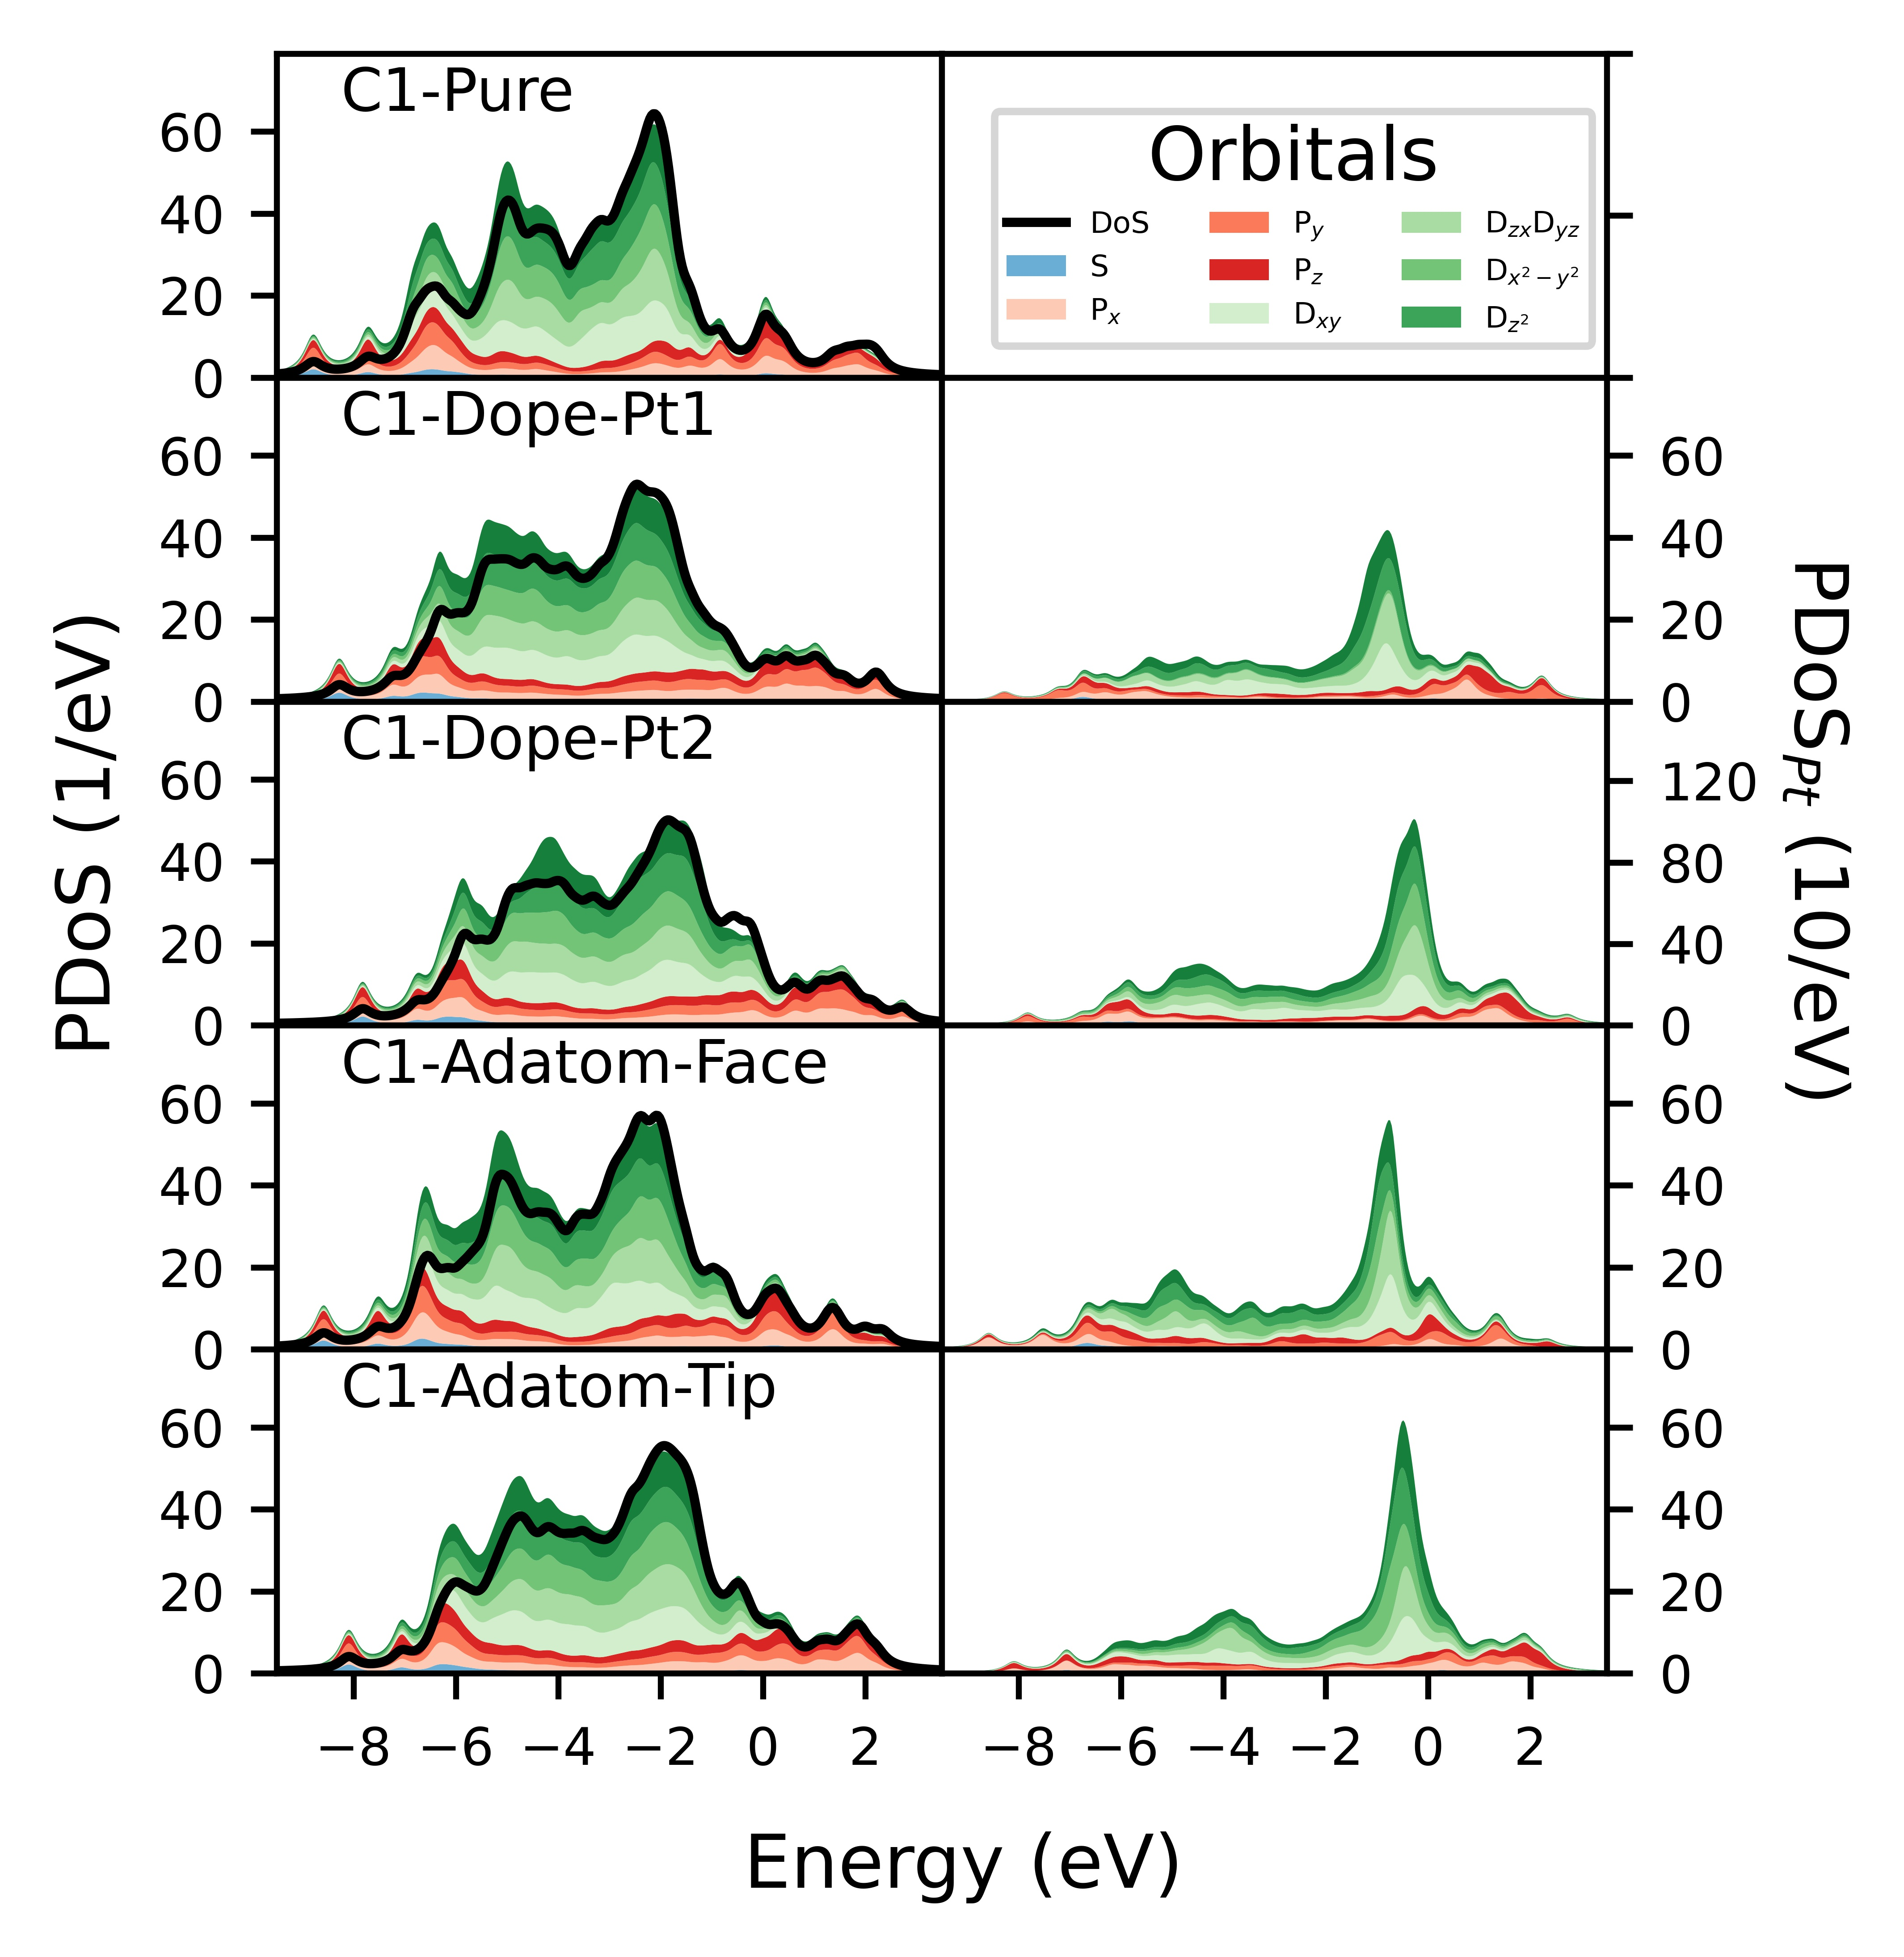
\includegraphics[width=\textwidth]{figures/LM/AuPt_EPJ/C1DoS.jpeg}
    \caption{Au$_{20}^{C1}$} 
    \label{Fig:C1Dos}
\end{subfigure}
\begin{subfigure}[b]{0.45\textwidth}
    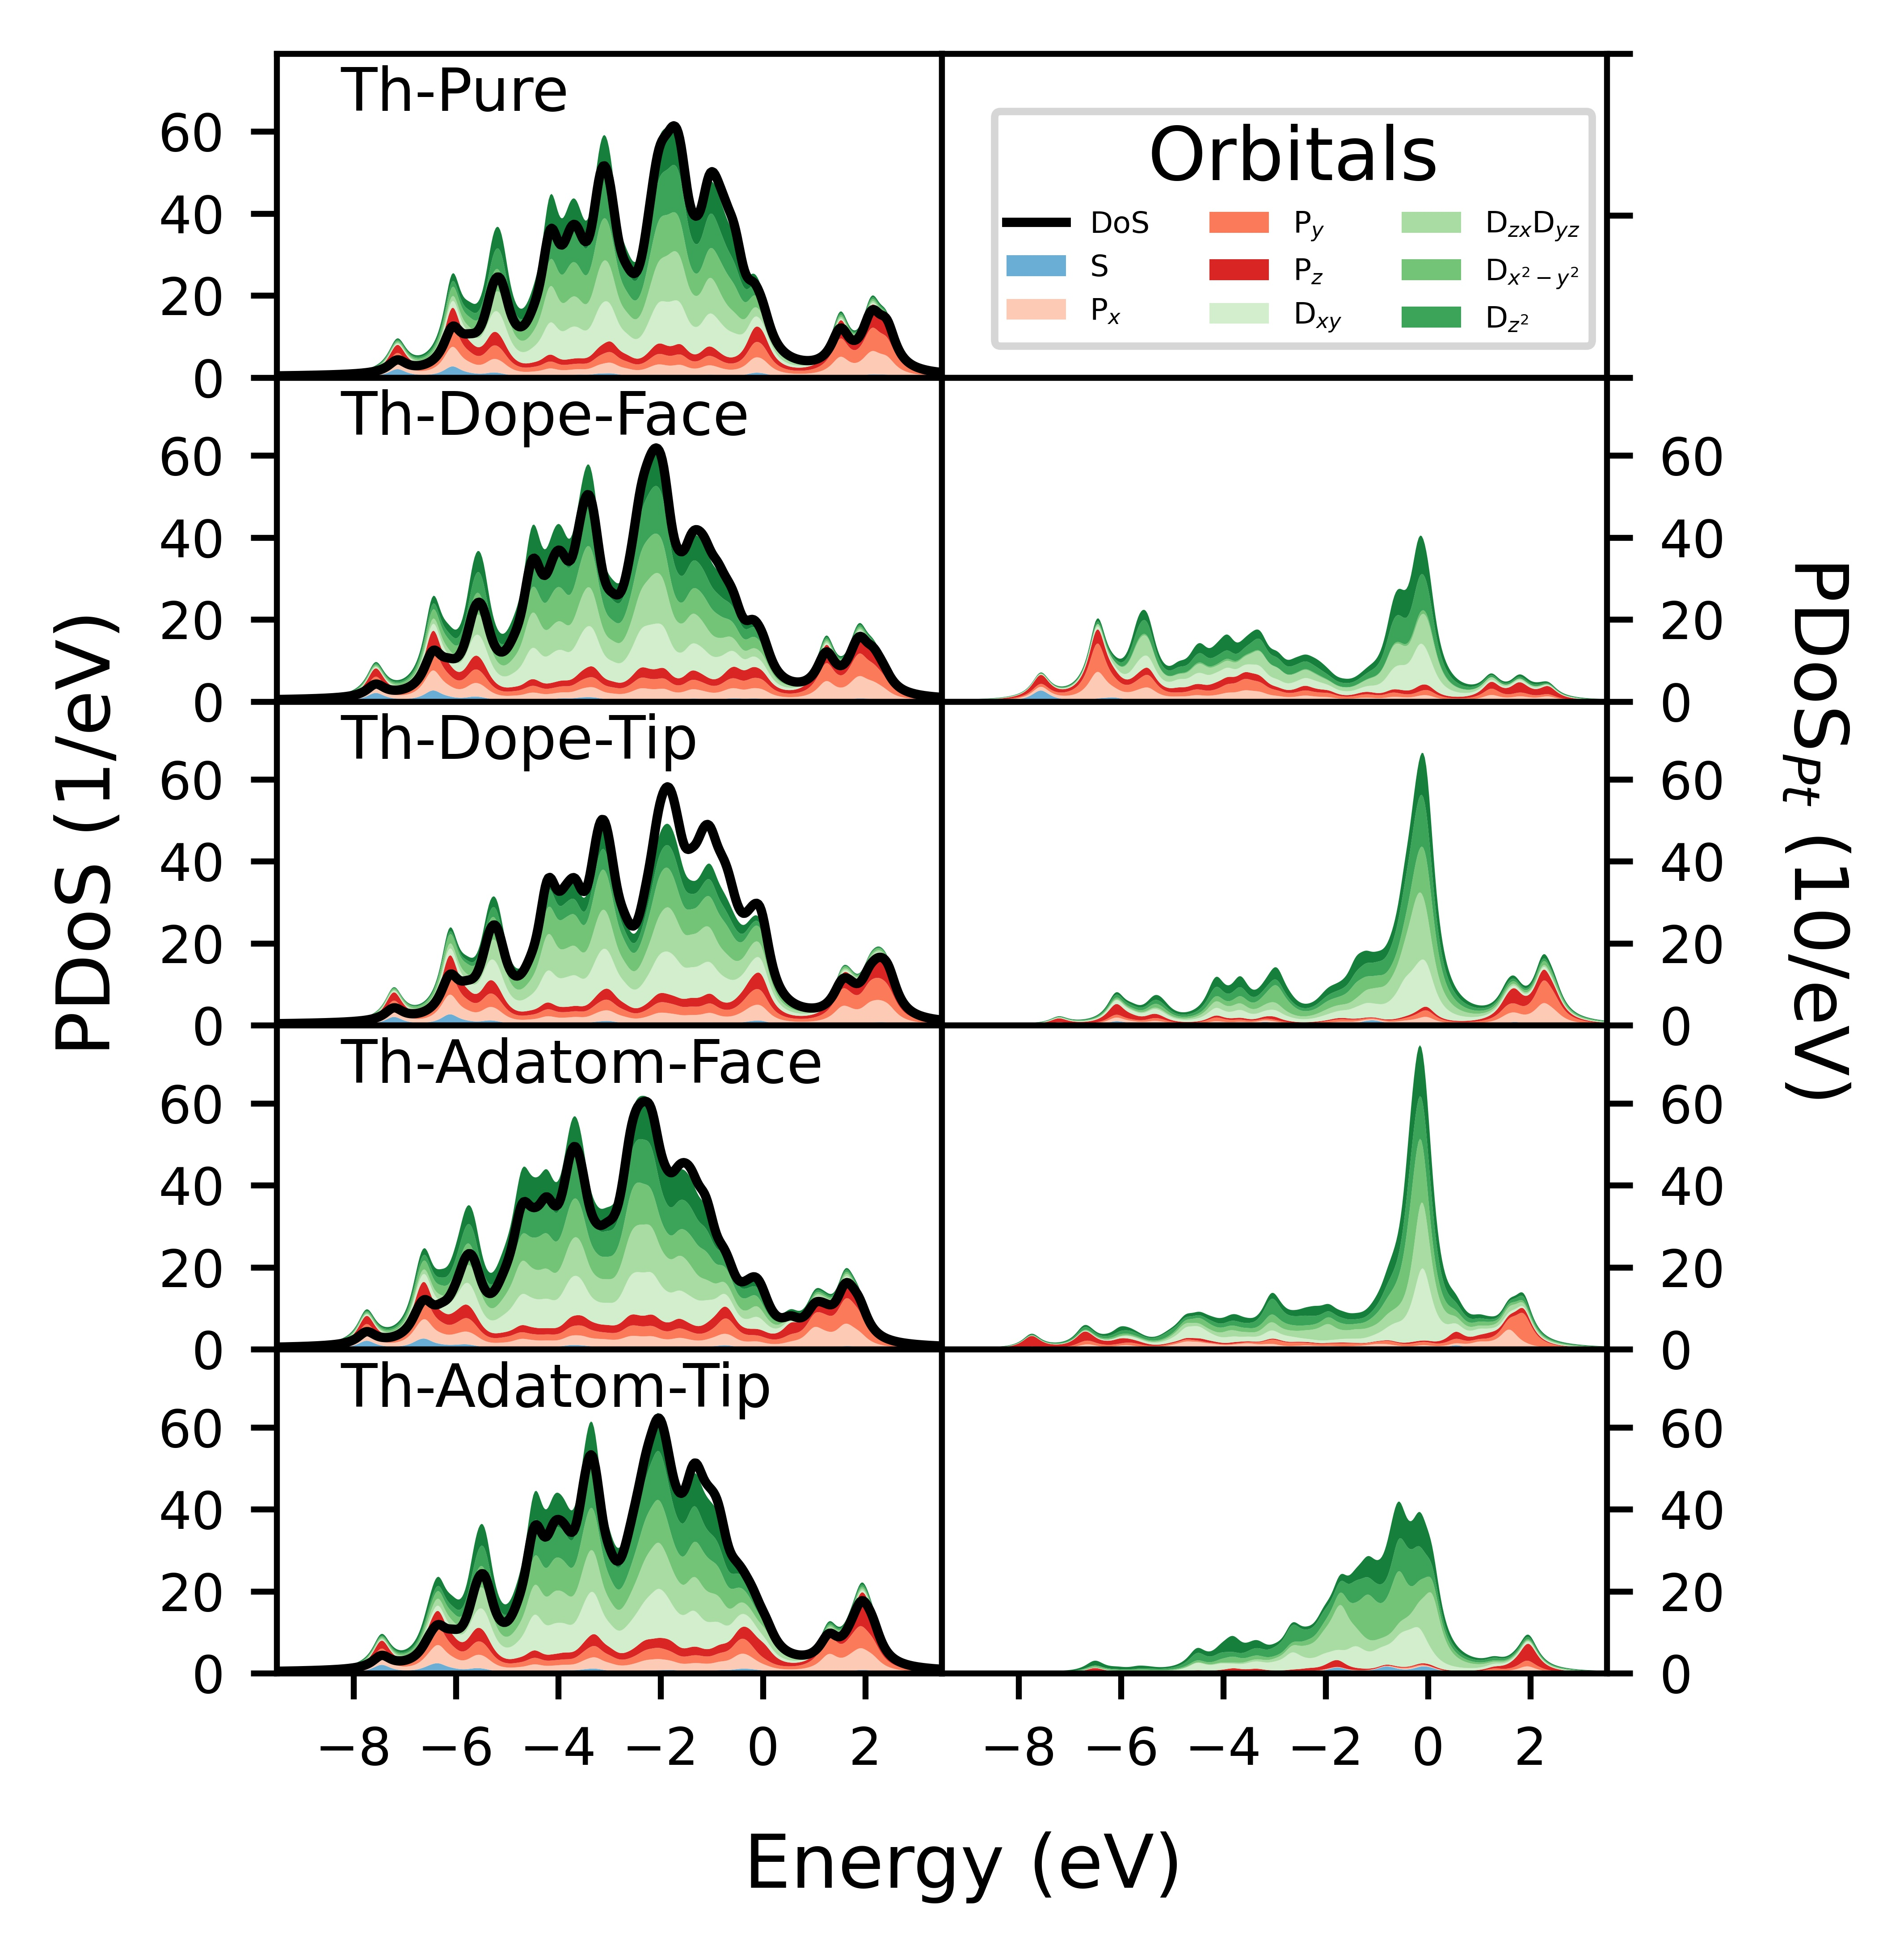
\includegraphics[width=\textwidth]{figures/LM/AuPt_EPJ/ThDoS.jpeg}
    \caption{Au$_{20}^{Th}$}
    \label{Fig:ThDos}
    \end{subfigure}
    \caption{Variation in the atomic projected density of states for the C1 candidate structures - left column of Figure \ref{Fig:Sites}. Top left in each sub-figure are the pure structures only. Left panels of each sub-figure illustrate the atomic PDoS for systems as they appear in Figure \ref{Fig:Sites}. Right panels in panels \textbf{a.} and \textbf{b.} present the atomic PDoS contributed from Pt only for their corresponding systems. Each plot has the total DoS presented as a black curve.}
    \label{Fig:AuPt_PDoS}
\end{figure}

In Figure \ref{Fig:DFT_Spec}, we present the absorption spectra as computed quantum mechanically via Eq. \ref{eqn:DFTSigma}, averaging over the contributions from each of the orthonormal propagation vectors, $\sigma_{abs}=\mathrm{Tr}\hat\sigma{_\mathbf{u}}/3$. We note that for the reported wavelengths, we may consider our NAs to be sufficiently within the quasi-static approximation - reporting wavelengths upwards from 300 nm compared to an approximate NA size of 1 nm.

\begin{figure}[ht!]
    \centering
    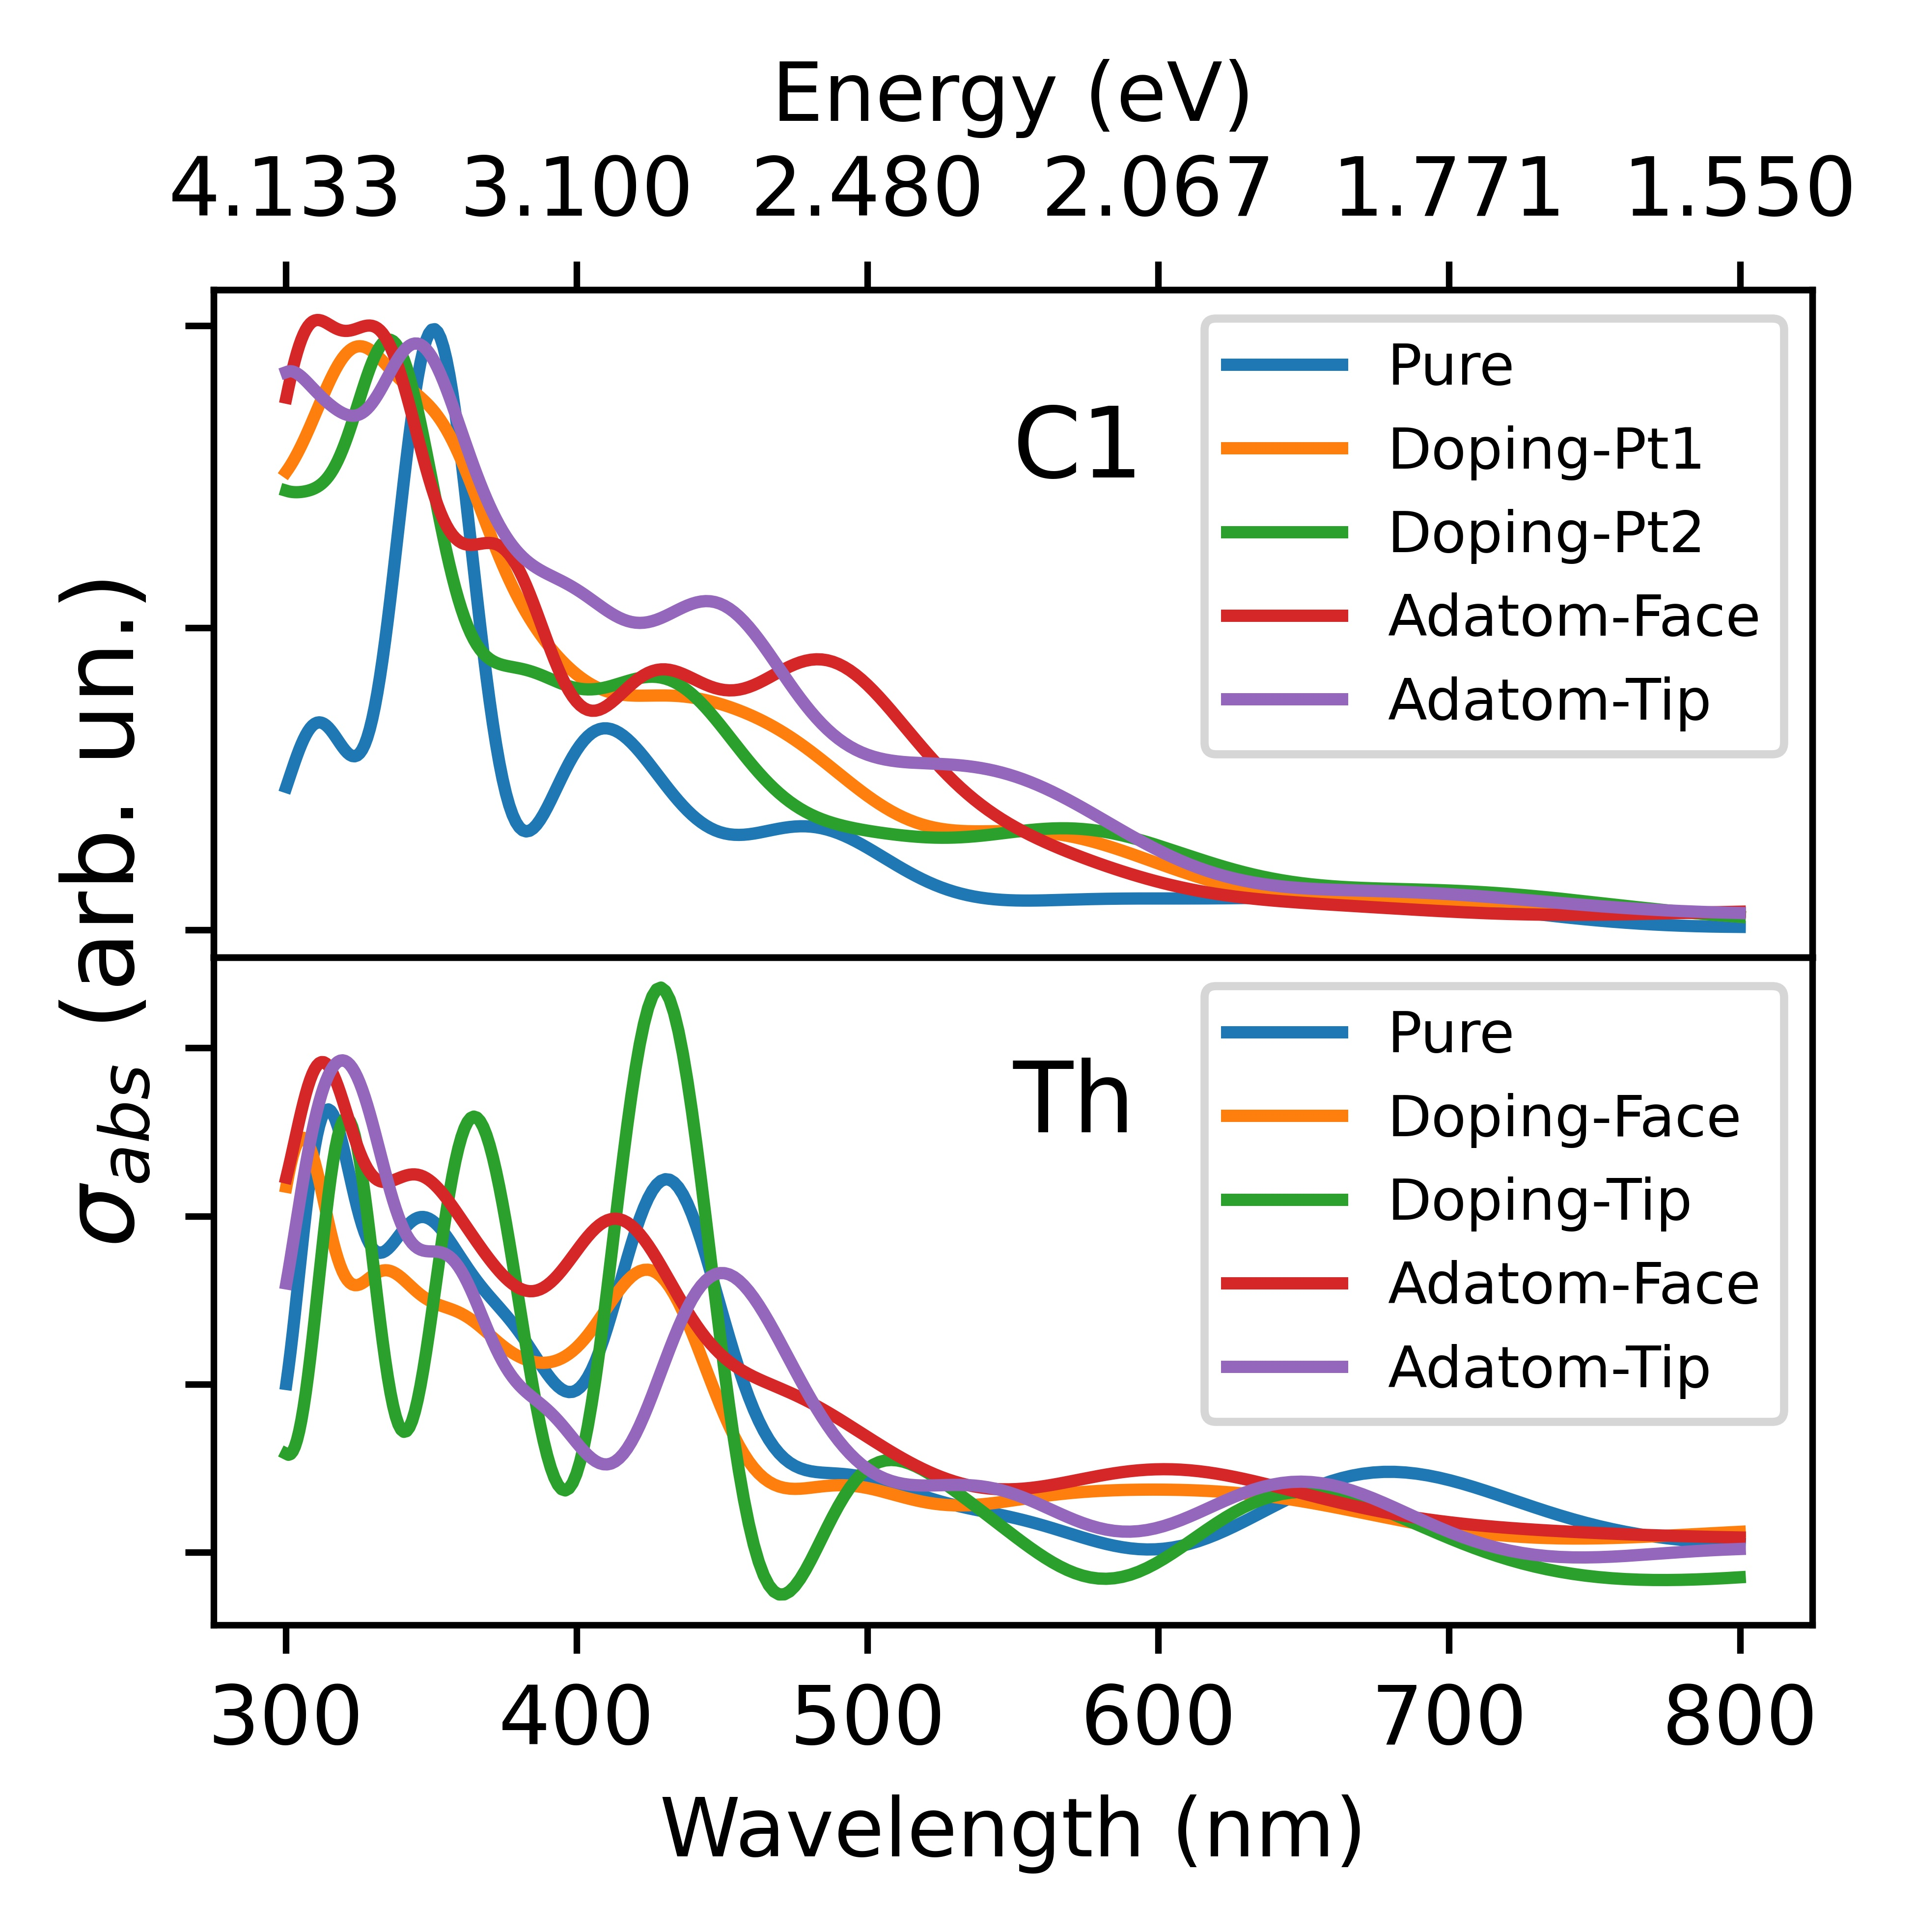
\includegraphics{figures/LM/AuPt_EPJ/Spectra_Abs.jpeg}
    \caption{Absorption and emission spectra of the Au$_{20}^{C1}$ - upper - isomer and its derivative structures; and the Au$_{20}^{Th}$ - lower - isomer and its derivative structures as computed via TDDFT methods.}
    \label{Fig:DFT_Spec}
\end{figure}


By first evaluating the atomic PDoS of Figure  \ref{Fig:C1Dos} and Figure \ref{Fig:ThDos} with respect to the reported $\varepsilon_{G}$ of Table \ref{tab:table}, we note that not only does the gap strongly depend on the geometry and chemical composition of the structure, but so too does the characteristic of the orbitals which flank this gap. Indeed, this may account for some of the observed behaviour in the computed absorption spectra of Figure \ref{Fig:DFT_Spec} in that the introduction of Pt as an adatom on the tip may serve to enhance some modes at lower frequencies.

By considering the fundamental relationship between occupied and unoccupied states, and photo-absorption spectra we begin to identify potential optically active modes, which may have a plasmonic characteristic in origin even at the sub-nanometric scale. It is understood that optically active modes may be excited by either interband transitions from the $d$ to the $sp$ orbitals, or by intraband transitions within $sp$ orbitals. In each case, the process must respect the conservation of angular momentum. Hence, we consider the distribution of orbital characteristics around the HOMO and LUMO as excitations are most likely to have their origin in states at and near to this region. There are strong $p$ and $d$ type orbitals near the HOMO~-~LUMO for all of the considered structures which suggests the existence of a rich array of angular momenta for the considered states. Moreover, by considering the right columns of Figure \ref{Fig:C1Dos} and Figure \ref{Fig:ThDos}, we see that the introduction of Pt has resulted in a strong delocalisation and hybridisation of states primarily centred at or near the HOMO. As such, excitations arising from the incidence of photons of a suitable frequency have an increased likelihood of being localised at this Pt impurity. Indeed, this is precisely what is desirable, as the Pt has been described as an excellent catalyst for the water-splitting reaction. This reaction requires hot carriers as reagents. Hence, by having an increased propensity to localise hot carriers around Pt, is likely to improve the performance of a prospective plasmon-enhanced catalyst. This localising effect is seen most strongly in the less symmetric C1 structure, relative to the high symmetry of the Au tetrahedron. It is possible that this strong local character may arise from a lack of symmetry within the structure and will surely be a point of increased scholarly intrigue.

By monitoring the atomic PDoS relative to the HOMO - LUMO gap listed in Table \ref{tab:table}, and comparing this information to the optical absorption spectra, seen in Figure \ref{Fig:DFT_Spec}, we conclude that the lack of absorption at or around $\varepsilon_{G}$ suggests that many of these modes are forbidden. Likely this is due to the necessary conservation of angular momentum being violated should an electron attempt to undergo such a  transition. We note that multiple absorption peaks can be observed in the UV~-~vis~-~NIR absorption spectra for each considered structure, which may arise from single-electron transitions \cite{ThreeStages}. Indeed, the relative smoothness of the Au$_{20}^{C1}$ and its derivative structures' spectra compared to those of the family of Au$_{20}^{Th}$ suggests that the nature of a given excitation may be profoundly different between high and low symmetry NAs. We draw focus to the strong presence of peaks in the instance Au$_{19}^{Th}$Pt$_{1}^{Tip}$, whose gap was computed to be 1.55 eV, and observe the presence of three strong peaks (Figure \ref{Fig:DFT_Spec}, green curve on the lower panel) in the UV-vis-NIR range. Compare this with Au$_{20}^{C1}$, whose gap is 50 times smaller at 0.03 eV and with a much smoother absorption spectrum in the same region with a visible peak at around 480 nm (Figure \ref{Fig:DFT_Spec}, blue curve on the upper panel). This may well be indicative of an LSPR-like response to the perturbation.

In the context of tetrahedra, the effects of symmetry~-~breaking have been studied by Zheng \textit{et al} \cite{C9NR08515G}, whose observations appear to agree with ours in that by losing the relatively rich T$_{d}$ symmetry one is able to introduce additional spectral features. However, it is worth acknowledging that in this work, the symmetry was broken through the rounding of vertices, not through doping with an alloying metal. Finally, the referenced study adopts a classical approach to modelling the plasmonic behaviour of Au MNPs.

We note that not only does alloying strongly influence the character of the optical properties, indeed the morphology, even between pure Au clusters, has profound influences. Given our results, we believe that the core message is abundantly clear - the richness of new behaviour by the simple process of doping a small cluster with one or two Pt atoms will lead to the emergence of many alternative optically active modes with a strongly hybridised character of states localised within the neighbourhood of the dopant. In particular, a Pt on a tip configuration enhances the absorption independently of the Au-isomer. In short, the relative position of the dopant, not solely the relative amount, has been found to be responsible for changes in the optical properties, making crucial the monitoring of the chemical ordering in NAs. Indeed, this observation cannot only be constrained to the symmetry of the doping site; but rather, as our analyses have demonstrated, to the morphology of the initial structure itself, thus making clear the profound interplay between morphology, chemical ordering in the alloyed phase, and the opto-electronic features of NAs.

\section{Discussion}

In this chapter, we have made comparisons between the Jellium and fully atomistic \textit{ab initio} models for computing opto-electronic properties of Au nanoparticles, identifying that whilst crude in its implementation - it is a reasonable comparison to draw when considering only the contribution of 6$s^{1}$ electrons. However, we have also shown that the contribution of lower lying 5$d^{10}$ orbitals appear to have a profound influence on the extinction spectra, hence their inclusion in the latter half of this chapter

We continued to show the utility and sensitivity of the GDM approach with respect to varying the metallic species, size, and morphology. This further motivates its utility in predicting the extinction spectra of mesoscale nanoalloys, as introduced in the following chapter.

Moreover, we have demonstrated the strong influence that the introduction of Pt may have on the static and optical properties of small Au cluster. We have considered the characteristic of the orbitals in the region of the HOMO and the LUMO, in conjunction with the size of the gap and the presence of given optical modes. By studying these nanoalloys at the level of TDDFT, we have been able to demonstrate how one may finely tune the optical properties, and even the localisation of potential hot carriers, by simply introducing Pt in a specific and targeted approach.

We hope this study will allow us to better understand how we may finely tune the optical and electronic characteristics of metallic nanoalloys - not only for the purposes of plasmon enhanced photo-catalysis, but for the broader community of those working in the beautiful world of nanoalloys.

